% -------------------------------------------------------- %
% Report for Isaac D. Scherson
% by: Dario Bahena Tapia
% by: Ricardo Zavaleta Vazquez
% by: Isai Barajas Cicourel


% -------------------------------------------------------- %
% Document Start
\documentclass[letter,12pt]{report}


% -------------------------------------------------------- %
% Packages
\usepackage{algorithmic}
\usepackage{amssymb}
\usepackage{amsfonts}
\usepackage{color}
\usepackage{xcolor}
\usepackage{amsopn}
\usepackage{graphicx}
\usepackage{caption}
\usepackage{listings}
\usepackage{listings,multicol}
\usepackage{graphicx}
\usepackage{hyperref}
\usepackage{cleveref}

\graphicspath{ {images/} }

\usepackage{listings}
\lstset{ %
  language=Java,
  basicstyle=\footnotesize,
  numbers=left
}
\lstdefinestyle{numbers}{numbers=left}
\lstdefinestyle{nonumbers}{numbers=none}

\usepackage{fancyvrb}
\fvset{fontsize=\scriptsize}
\RecustomVerbatimEnvironment{verbatim}{Verbatim}{}

% -------------------------------------------------------- %
% Commands
\newcommand{\C}[1]{\emph{#1}}
\newcommand{\bigO}[1]{\ensuremath{\operatorname{O}\left(#1\right)}}

% -------------------------------------------------------- %
% Document
\begin{document}


% --------------------------- %
% Title Page Start
% --------------------------- %
\begin{titlepage}
\begin{center}

~\\[4 cm]


\includegraphics[width=15 cm]{Oracle_Logo.pdf}

~\\[0.5 cm]

% Document Information
{\LARGE Multiprocessor Programming Course} \\[0.2 cm]

% Names
{Dario Bahena Tapia - Ricardo Zavaleta Vazquez - Isai Barajas Cicourel}

% Date
{\small December 2015}

\end{center}
\end{titlepage}
% --------------------------- %
% Title Page End
% --------------------------- %

\tableofcontents

\chapter{Introduction}
\include{./sections/Intro}

% --------------------------- %
% ch 02 Mutual Start
% --------------------------- %
\chapter{Mutual Exclusion}
\section{\textbf{LockFreeQueueTest}}

\subsection{Particular Case (problem)}
This is a particular case of the mutual exclusion problem, where the
shared resource is a queue.

\subsection{Solution}
In order to guarantee the correctness of
the multi-threaded access to the queue, it implements a lock free
scheme on its \C{enq} and \C{deq} methods by putting waits
before modifying the state of the queue. It does it incorrectly
though, as we will see later. \\

\begin{lstlisting}[style=numbers]
class LockFreeQueue {
  public int head = 0;   // next item to dequeue
  public int tail = 0;   // next empty slot
  Object[] items; // queue contents
  public LockFreeQueue(int capacity) {
    head = 0; tail = 0;
    items = new Object[capacity];
  }

 public void enq(Object x) {
     // spin while full
     while (tail - head == items.length) {}; // spin
     items[tail % items.length] = x;
     tail++;
  }

  public Object deq() {
      // spin while empty
      while (tail == head) {}; // spin
      Object x = items[head % items.length];
      head++;
      return x;
  }
}
\end{lstlisting}
\hfill

\subsection{Experiment Description}
The test program LockFreeQueueTest includes the following individual
test cases; the parallel degree is two threads for each operation
(queue or dequeue), with a TEST\_SIZE of 512 (number of items to
enqueue and dequeue) which is spread evenly among the two threads on
each group:

\begin{itemize}
  \item \C{testSequential}: calls \C{enq} method as many times as
    TEST\_SIZE, and later calls \C{deq} method the same number of
    times checking that the FIFO order is preserved. 
  \item \C{testParallelEnq}: enqueues in parallel (two threads) but dequeues
    sequentially.
  \item \C{testParallelDeq}: enqueues sequentially but dequeues in
    parallel (two threads)
  \item \C{testParallelBoth}: enqueues and dequeues in parallel (with
    a total of four threads, two for each operation).
\end{itemize}

\subsection{Observations and Interpretations}
The bottom line of this exercise is most likely, to show several types
of problems that can occur if we do not use mutual exclusion; the
queue implementation fails implementing it, making the test vulnerable
to several cases of race conditions. Below we explain some of them.

\subsubsection{Non atomic dequeue: referencing invalid registers}

The symptom for this problem is a NullPointerException: \\

\begin{verbatim}
There was 1 error:
1) testParallelEnq(mutex.LockFreeQueueTest)java.lang.NullPointerException
	at mutex.LockFreeQueueTest.testParallelEnq(LockFreeQueueTest.java:69)
	at sun.reflect.NativeMethodAccessorImpl.invoke0(Native Method)
	at sun.reflect.NativeMethodAccessorImpl.invoke(NativeMethodAccessorImpl.java:62)
	at sun.reflect.DelegatingMethodAccessorImpl.invoke(DelegatingMethodAccessorImpl.java:43)
\end{verbatim}
\hfill

where the offending line is a cast to an Integer from the value
returned by the \C{deq} method; this implies that such function is
returning \C{null}. A possible scenario to produce this outcome is as
follows. Prefixes of T1 or T2 indicate the thread running the action,
and they refer to the line numbers of the code of method \C{deq}
posted above.

\begin{itemize}
\item Assume that queue holds a single element which lives in \C{items}
  array at position 0; the array has \C{null} on position 1 (per
  initialization).
\item T1: Executes method up to line 20. 
\item T2: Executes method up to line 19. 
\item T1: Executes line 21, getting \C{items[0]}. 
\item T2: Executes line 20, but as \C{head} was changed already, it
  gets \C{items[1]}.  
\item T1: Executes line 22 returning \C{items[0]}
\item T2: Executes line 22 returning \C{items[1]}, which was \C{null}.
\end{itemize}
\hfill

The problem with above interlacing derives from the fact that the
\C{deq} method is not an atomic operation, hence it allowed both threads to
enter into the critical section and compete for updating the shared
variables. 

\subsubsection{Non atomic dequeue: returning duplicate values}

The symptom for this problem is a duplicate pop warning: \\

\begin{verbatim}
.parallel both
.sequential push and pop
.parallel enq
E.parallel deq
Exception in thread "Thread-7" junit.framework.AssertionFailedError: 
DeqThread: duplicate pop
	at junit.framework.Assert.fail(Assert.java:47)
	at mutex.LockFreeQueueTest$DeqThread.run(LockFreeQueueTest.java:132)
\end{verbatim}
\hfill

where the offending line is an assertion that validates that nobody
else has pop such value from the queue; as the threads which populate
do have non overlapping ranges of values, the pop operations (\C{deq})
shall never return a duplicate one. But duplication is possible
indeed, if we have a sequence like the one below between the two threads:

\begin{itemize}
\item Assume that queue holds a single element which lives in \C{items}
  array at position 0.
\item T1: Executes method up to line 19. 
\item T2: Executes method up to line 19. 
\item T1: Executes line 20, getting \C{items[0]}.
\item T2: Executes line 20, getting as well \C{items[0]}.
\item T1: Executes line 21, setting \C{head} to 1.
\item T2: Executes line 21, setting \C{head} to 2.
\item T1: Executes line 22 returning \C{items[0]}.
\item T2: Executes line 22 returning \C{items[0]}.
\end{itemize}
\hfill

Not only we left the queue in an inconsistent state (head has
incorrect value), but we also returned the same element twice,
triggering then the violation on the test. The underlying problem is
the same as previous case: lack of atomicity of the \C{deq} method.

\subsubsection{Non atomic auto-increment: loosing values}

The symptom for this problem is a never ending program, hanging on the
test \C{testParallelBoth}. When produced several thread dumps of the
Java program, we can see two hanging threads: \\

\begin{verbatim}
"Thread-7" #16 prio=5 os_prio=0 tid=0x00007f3140102000 nid=0x3f51
           runnable [0x00007f31226e9000]
   java.lang.Thread.State: RUNNABLE
	at mutex.LockFreeQueue.deq(LockFreeQueue.java:33)
	at mutex.LockFreeQueueTest$DeqThread.run(LockFreeQueueTest.java:141)

"main" #1 prio=5 os_prio=0 tid=0x00007f3140009800 nid=0x3f3c in Object.wait() 
          [0x00007f3148382000]
   java.lang.Thread.State: WAITING (on object monitor)
	at java.lang.Object.wait(Native Method)
	- waiting on <0x00000000d6effea8> (a mutex.LockFreeQueueTest$DeqThread)
	at java.lang.Thread.join(Thread.java:1245)
	- locked <0x00000000d6effea8> (a mutex.LockFreeQueueTest$DeqThread)
	at java.lang.Thread.join(Thread.java:1319)
	at mutex.LockFreeQueueTest.testParallelBoth(LockFreeQueueTest.java:123)
	at sun.reflect.NativeMethodAccessorImpl.invoke0(Native Method)
	at sun.reflect.NativeMethodAccessorImpl.invoke(NativeMethodAccessorImpl.java:62)
	at sun.reflect.DelegatingMethodAccessorImpl.invoke(DelegatingMethodAccessorImpl.java:43)
	at java.lang.reflect.Method.invoke(Method.java:497)
	at junit.framework.TestCase.runTest(TestCase.java:164)
	at junit.framework.TestCase.runBare(TestCase.java:130)
\end{verbatim}
\hfill

The main thread is waiting for a dequeue thread to finish; but that
one is on an infinite loop at line 19 of \C{deq} method (line numbers
per our listing in this document, not in the file). This means that we
have lost some of the inserted elements in queue, and that one of the
dequeue threads will never finish; as they expect each to pop a fixed
amount of elements per the test. \\

But the amount of times we request a dequeue operation, among all
threads, is the same as the number of elements we queued; how come we
end up loosing some of those? One possible explanation is again, the
lack of atomicity but this time of the \C{enq} method; to be more
specific, the lack of atomicity of its auto-increment operation 
\C{tail++} (line 14). Let us remember that the auto-increment
operator in Java is nothing but syntactic sugar for the following
sequence of operations (when applied to \C{tail} variable): \\

\begin{lstlisting}[style=nonumbers]
  tmp = tail;
  tmp = tmp + 1;
  tail = tmp;
\end{lstlisting} 
\hfill

If two threads execute the lower level operations above, we can see
how they can end up loosing increments in the shared variable
\C{tail}; the following sequence is on example of such scenario:

\begin{itemize}
\item T1: executes \C{tmp = tail}.
\item T2: executes \C{tmp = tail}.
\item T1: executes \C{tmp = tmp + 1}.
\item T2: executes \C{tmp = tmp + 1}.
\item T1: executes \C{tail = tmp}.
\item T2: executes \C{tail = tmp}.
\end{itemize}
\hfill

We can appreciate that in the above interlacing, the final value of
the shared variable is $\C{tail} + 1$; instead of the expected value
of $\C{tail} + 2$. It would be enough to loose a single value this
way, in order to make the enqueue threads think that they inserted the
total of 512, while they really inserted 511; as each dequeue thread
will try to pop 256 each, only one of them will be able to finish
while the other will get blocked after having removed 255
entries. That is most likely the explanation for the hung threads we
pasted above \footnote{Note that it does not matter that the array
  \C{items} has populated all the correct entries, because the flow is
  controlled by the counters \C{tail} and \C{head}.}; the solution is
again to really implement mutual 
exclusion around the methods \C{deq} / \C{enq}; in such a way that
they become atomic operations.

\subsection{Proposed changes to fix the problems}

All the three scenarios described before can be eliminated, if we make
the methods \C{enq} and \C{deq} atomic; this can be easily achieved in
Java by making them \C{synchronized}. However, by doing that, we will
loose parallelism among the two groups of threads (those calling
\C{enq} and those calling \C{deq}); this is because the
\C{synchronized} keyword uses as lock the whole object, so at any
moment in time, only one synchronized method can actually run within any object. In
order to overcome this limitation, we can use synchronized blocks
against two different lock objects (one for each operation). \\

Even with the changes above, we can still have issues; what if the
very first thread running is one calling \C{deq} method? It will find
the queue empty and loop forever. In order to prevent that, we should
remove the waiting operation out of the queue methods, and put them in
the test code itself. This is because, on the cited scenario that we
try to dequeue with an empty queue, we would expect to simply try
again (giving the chance to parallel enqueue threads to produce something for
us to pop). The final code which incorporates these fixes is listed
below: \\

\newpage
\begin{lstlisting}[style=numbers]
class LockFreeQueue {
  private static Object enqLock = new Object();
  private static Object deqLock = new Object();
    
  public int head = 0;   // next item to dequeue
  public int tail = 0;   // next empty slot
  Object[] items; // queue contents
  public LockFreeQueue(int capacity) {
    head = 0; tail = 0;
    items = new Object[capacity];
  }

 public  boolean enq(Object x) {
     synchronized(enqLock)
         {
             if (tail - head == items.length) {
                 return false;
             }
             items[tail % items.length] = x;
             tail++;
             return true;
         }
  }

  public Object deq() {
      synchronized(deqLock)
          {
              if (tail == head) {
                 return null;
              }
              Object x = items[head % items.length];
              head++;
              return x;
          }
  }
}

\end{lstlisting}
\hfill
\newpage

The test code was also modified, to make the enqueue and dequeue
threads to iterate until they have successfully called their
respective methods 256 times (total size of queue divided by number of
threads). A successful call is one that does not return \C{false} nor
\C{null}. The modified code was executed ten thousand times and it did
not produce any of the original problems we explained. Though not a
formal proof of its correctness, it is a good indication of the same
(the original program produced one of the cited problems quite often,
usually within 10 executions).



../../zava/Multiprocessor//Peterson.tex
% --------------------------- %
% Bakery Start
% --------------------------- %
\section{\textbf{Bakery Test}}
%%%%%%%%%%%%%%%%%%%%%%%%%%%%%%%%%%
\subsection{Particular Case}
\par
In this experiment, we are dealing with the problem of mutual exclusion with a
number of participants $>2$.
\par
We have already seen that Peterson Algorithm works for two threads. It garantees
mutual exclusion and is starvation free. Therefore, the algorithm is deadlock
free. Now let us focus in an algorithm that can be used to coordinate more
threads.
\par
%%%%%%%%%%%%%%%%%%%%%%%%%%%%%%%%%%
\subsection{Solution}
\par
The algorithm that we will play with is called \textit{Bakery}. Its name comes from the
fact that it is similar to the protocol used in bakeries where one enters the
store and picks a number that indicates the order in which each client will be
attended. 
\par
In the algorithm, the fact of entering the store is done by setting a flag.
After that, the thread calculates the next number in the machine. 
\par
The algorithm then chooses the next number to be attended. When that happens,
the thread is allowed to enter the critical section.
\par
One thing that we ougth to mention is that threads can have the same number
assigned. If that is the case, the next in the line is decided using a
lexicographical ordering of the threads ids.
\par
Here we show the interesting methods used in this algorithm:
\par
\hfill
\begin{lstlisting}[style=numbers]
  public void lock() {
    int me = ThreadID.get();
    flag[me]  = true;
    int max = Label.max(label);
    label[me] = new Label(max + 1);
    while (conflict(me)) {};  // spin
  }

  public void unlock() {
    flag[ThreadID.get()] = false;
  }
  
  private boolean conflict(int me) {
    for (int i = 0; i < label.length; i++) {
      if (i != me && flag[i] && label[me].compareTo(label[i]) < 0) {
        return true;
      }
    }
    return false;
  }

  static class Label implements Comparable<Label> {
    int counter;
    int id;
    Label() {
      counter = 0;
      id = ThreadID.get();
    }
    Label(int c) {
      counter = c;
      id = ThreadID.get();
    }
    static int max(Label[] labels) {
      int c = 0;
      for (Label label : labels) {
        c = Math.max(c, label.counter);
      }
      return c;
    }
    
    public int compareTo(Bakery.Label other) {
      if (this.counter < other.counter
          || (this.counter == other.counter && this.id < other.id)) {
        return -1;
      } else if (this.counter > other.counter) {
        return 1;
      } else {
        return 0;
      }
    }
  }
\end{lstlisting}
\hfill
\par
In the \textit{lock()} method, we observe that the thread signals its intention
of accessing the critical section by setting its flag to true. After that, the
thread picks its number and then it sits and waits for its turn. The thread has
to wait if another thread which announced its intention to use the resource has
a smaller label. 
\par
%%%%%%%%%%%%%%%%%%%%%%%%%%%%%%%%%%
\subsection{Experiment Description}
\par
Now let us explain how the experiments work. In this case we have 8 threads
increasing a counter from 0 to 1024. Each thread will increase the counter 128
times. At the end, the counter must remain in 1024. If that is not the case,
then there is a problem with the mutual exclusion algorithm.
\par
%%%%%%%%%%%%%%%%%%%%%%%%%%%%%%%%%%
\subsection{Sample Results}
\par
In this exercise we observed that in the machine that we have been using, the
test for the Bakery algorithm fails consistently with the following error:
\par
\begin{verbatim}
.F
Time: 0.019
There was 1 failure:
1) testParallel(mutex.BakeryTest)junit.framework.AssertionFailedError:
expected:<1019> but was:<1024>
        at mutex.BakeryTest.testParallel(BakeryTest.java:47)
        at sun.reflect.NativeMethodAccessorImpl.invoke0(Native Method)
        at
sun.reflect.NativeMethodAccessorImpl.invoke(NativeMethodAccessorImpl.java:57)
        at
sun.reflect.DelegatingMethodAccessorImpl.invoke(DelegatingMethodAccessorImpl.java:43)

FAILURES!!!
Tests run: 1,  Failures: 1,  Errors: 0
\end{verbatim}
\par
%%%%%%%%%%%%%%%%%%%%%%%%%%%%%%%%%%
\subsection{Interpretation}
\par
Let us elaborate on the meaning of the error that we got. The assertion failure
says that at the end of the algorithm, our counter didn't reach the expected
1024. This problem might indicate that our counter wasn't actually being
protected by the lock because it looks like multiple threads found the counter
with a value of $i$ and increased it to $i+1$. This is wrong.
\par
After investigating the problem in more detail, we found out that the problem in
this code has to do with the way the \textit{label} array is accessed and
modified. For example, in the lock method, multiple threads can reach the point
where the max is calculated and hence these mutiple threads can take the same
turn. The algorithm takes care of this problem by introducing a lexicographical
ordering in the comparison: if two threads have the same number, the decision is
made based on the $threadID$.
\par
Also, as explained in the textbook, we cannot be sure that we have a correct
memory consistency: it is possible that the processor modified the order in
which operations in the \textit{lock()} method are executed. It is also possible
that the processor decided to execute an instruction before another.
\par
%%%%%%%%%%%%%%%%%%%%%%%%%%%%%%%%%%
\subsection{Proposed solution}
\par
The following fragment of code shows one possible way of fixing the code:
\par
\hfill
\begin{lstlisting}[style=numbers]
  public void lock() {
    int me = ThreadID.get();
    flag[me]  = true;
    synchronized (label){
      int max = Label.max(label);
      label[me] = new Label(max + 1);
      while (conflict(me)) {};  // spin
    }
  }
\end{lstlisting}
\hfill
Note that this solution is not quite satisfactory as we are basically using a
Java mechanism to ensure synchronized access in an algorithm that promises to
provide synchronized access.
\par
In any case, let us show the output of the program after this fix:
\begin{verbatim}
.
Time: 0.015

OK (1 test)
\end{verbatim}
\hfill
\par
After the fix the results in the proposed system were all OK. In all cases, the
threads were able to cooperate to increase the counter to 1024.
\par
One thing that is worth mentioning is that unlike the Peterson Algorithm, for
example, the Bakery algorithm is able to coordinate multiple threads (at least
in theory). This fact was shown in the test case were 8 threads were coordinated
to increase the counter.
%%%%%%%%%%%%%%%%%%%%%%%%%%%%%%%%%%
% --------------------------- %
% Bakery End
% --------------------------- %

% -------------------------------------------------------- %
% Filter Lock
% by: Isai Barajas Cicourel


% -------------------------------------------------------- %
% Document Start

\section{\textbf{Filter Lock}}


% -------------------------------------------------------- %
% Particular Caes

\subsection{Particular Case}
\par
In this experiment, the particular case we are trying to study is mutual exclusion where several threads try to use a shared resource.
\par
We are trying to do so using waiting rooms called levels that a thread must traverse before acquiring the lock.
\par


% -------------------------------------------------------- %
% Solution Information

\subsection{Solution}
\par
We now consider two mutual exclusion protocols that work for $n$ threads, where $n$ is greater than $2$. The Filter lock, is a direct generalization of the Peterson lock to multiple threads.
\par
The Filter lock, creates \(n - 1\) ``waiting rooms'', called levels, that a thread must traverse before acquiring the lock. The Peterson lock uses a two-element boolean flag array to indicate whether a thread is trying to enter the critical section. The Filter lock generalizes this notion with an $n$-element integer $level[]$ array, where the value of $level[A]$ indicates the highest level that thread $A$ is trying to enter. 
\par


% -------------------------------------------------------- %
% Experiment

\subsection{Experiment Description} 
\par
The test creates $8$ threads that need to be coordinate in order to increment a common counter. All threads have to cooperate to increase this counter from 0 to $1024$. Each of the threads will increase by one the counter $128$ times.
The expected result is that regardless of the order in which each thread executes the increment, at the end the counter must stay at $1024$.
If that is not the case, then it means that mutual exclusion did not work.
\par

% -------------------------------------------------------- %
% Results

\subsection{Observations and Interpretations}

\par
When executing the test on a dual core machine there was a a low chance of failure, but when executed on a Quad core and Six core machines the problems where more consistent.
\begin{lstlisting}[frame=single]
Testcase: testParallel(mutex.FilterTest):	FAILED
expected:<1023> but was:<1024>
\end{lstlisting}


% -------------------------------------------------------- %
% Results

\subsection{Proposed changes to fix the problem}

\par
Even do the victim and level arrays are \textit{volatile}, the atomicity is not guarantee and so to fix this I added the \textit{synchronized} reserved word to the \textit{sameOrHigher()} method in order to guarantee atomicity while checking the levels.
\begin{lstlisting}[frame=single,breaklines=true]
// Is there another thread at the same or higher level?
private synchronized boolean 
  sameOrHigher(int me, int myLevel) {
  for (int id = 0; id < size; id++)
    if (id != me && level[id] >= myLevel) {
      return true;
    }
    return false;
}
\end{lstlisting}
Once the change is made the execution works fine on every equipment used.
\begin{lstlisting}[frame=single,breaklines=true]
Script Directory: .
Using OS: Linux
Linux Java 6 Runtime: ./jre/linux/bin
Will execute test from input: mutex.FilterTest
Classpath: .:./lib/*:./output/:./build/
Running JUnit using Linux
JUnit version 4.12
.
Time: 0.021

OK (1 test)
\end{lstlisting}


% -------------------------------------------------------- %
% Why?

\subsection{Proposed solution}
\par
Once the comparing of the level was made atomic, the spin made for conflicting threads was properly working and able to cooperate to increase the counter to 1024.
\par
One thing that is worth mentioning is that the \textit{volatile} keyword seems to either have an implementation problem or not documented restriction, since it is not helping guarantee the use of the waiting rooms causing additional increases in the counter, thus ending with a different number rather than the one expected.


\section{\textbf{QueueTest}}

\subsection{Particular Case (problem)}
The problem we want to solve is again mutual exclusion around a shared
bounded queue; just like chapter 2. The difference here is that, instead of
just using locks the authors try to explain the facilities provided by
Java \C{Condition} interface (part of package
\C{java.util.concurrent.locks}). Such interface, along with the
\C{Lock} one, offer a finer grain control over the
Monitors \footnote{Monitors, as explained in the book, are an
  structured way to integrate synchronization with an object's data
  and methods (speaking about OO paradigm).}
capabilities offered by Java language; when compared to merely using
the \C{synchronized} feature. 

\subsection{Solution}
The solution to the mutual exclusion problem around the bounded queue is
solved by using a single Lock of type \C{ReentrantLock}, to control
exclusive access to the data structure (reentrant is important to
ensure that a thread which has gotten the lock already, can request it
again as many times as it want). In addition, the solution uses a
couple of \C{Condition} objects to represent the conditions 
which enqueuers and dequeuers wait on: \\

\begin{itemize}
  \item \C{notFull}: condition enqueuers wait on, prior daring to push.
  \item \C{notEmpty}: condition dequeuers wait on, prior daring to pop.
\end{itemize}
\hfill

The implementations of methods \C{enq} and \C{deq} are similar to
those from the flawed \C{LockFreeQueue} that we analyzed before; there
are a couple of crucial differences though: \\

\begin{itemize}
\item We use a lock to implement mutual exclusion, so we eliminate all
  the issues seen before due race conditions.
\item The potentially infinite loops for both \C{enq} and \C{deq} now
  do something: they call the \C{await} method on their respective
  conditions. This guarantees that we do not have deadlocks: if a
  thread does not find the queue on the expected state to perform the
  operation, it releases the lock and allow the others to proceed. In
  that way we allow enqueuers to put the data we are waiting for, or
  the dequeuers to make the space we need; after which they
  ``wake-up'' the waiting threads with a call to condition's
  \C{signal} method. 
\end{itemize}
\hfill

The code looks quite similar to our second proposed modification of previous
exercise \C{LockFreeQueueTest}; and actually, it also looks quite
similar to the sample code listed on the \href{http://docs.oracle.com/javase/7/docs/api/java/util/concurrent/locks/Condition.html}{Javadoc API of \C{Condition}
  interface} (on which we also based our proposal). Anyway, the book
solution is listed below for further reference: \\

\begin{lstlisting}[style=numbers]
class Queue<T> {
  final Lock lock = new ReentrantLock();
  final Condition notFull  = lock.newCondition();
  final Condition notEmpty = lock.newCondition();  
  final T[] items; 
  int tail, head, count;  
  public Queue(int capacity) {
    items = (T[])new Object[capacity];
  }
  public void enq(T x) throws InterruptedException {
    lock.lock();
    try {
      while (count == items.length)
        notFull.await();
      items[tail] = x;
      if (++tail == items.length)
        tail = 0;
      ++count;
      notEmpty.signal();
    } finally {
      lock.unlock();
    }
  }  
  public T deq() throws InterruptedException {
    lock.lock();
    try {
      while (count == 0)
        notEmpty.await();
      T x = items[head];
      if (++head == items.length)
        head = 0;
      --count;
      notFull.signal();
      return x;
    } finally {
      lock.unlock();
    }
  }
}
\end{lstlisting}
\hfill

\subsection{Experiment Description}

The test is pretty much the same than \C{LockFreeQueueTest}, except
for the number of threads (8 instead of 2) and data (64 instead of
512). 

\subsection{Observations and Interpretations}
Although the test does not exhibit any issue on 2 nor in 24 cores, we
would feel safer replacing the \C{signal} calls by \C{signalAll}, just
to totally discard the potential problem of lost wake-ups explained on
the book (this is what we did for our second proposal to fix
\C{LockFreeQueueTest}, indeed). A sample successful execution is shown
below: \\ 

\begin{verbatim}
$ junit monitor.QueueTest
.sequential push and pop
.parallel both
.parallel deq
.parallel enq

Time: 0.009

OK (4 tests)
\end{verbatim}
\hfill


% --------------------------- %
% Mutual End
% --------------------------- %

% --------------------------- %
% ch 04 Foundations Start
% --------------------------- %
\chapter{Foundations of Shared Memory}
\section{\textbf{Safe Boolean MRSW Register}}
% ------------------------------------------------------------------------------------ %
\subsection{Particular Case}
\par
In class we saw the difference between Safe, Regular and Atomic Registers. In
this excersice we are experimenting with a Safe Boolean Register. In particular,
we are trying a register that allows one single writer whose writen value can be
examined by multiple readers. We need to remember that Safe registers are those
that :
\begin{itemize}
\item If a read does not overlap with a write, then the read returns the last
written value
\item If a read overlaps with a write, then the read can return any value in the
domain of the register's values
\end{itemize}
% ------------------------------------------------------------------------------------ %
\subsection{Solution}
\par
One way to achive this behaviour is using a SRSW Safe register. The code that is
provided with the book does this by having a boolean SRSW register per thread,
in other words, it is an array of boolean values. When doing a write, the writer
iterates over this array and writes the new value. The readers simply access its
assigned slot in the array (based on the thread id) and return the stored value. 
% ------------------------------------------------------------------------------------ %
\subsection{Experiment Description}
\par
This program provides two test cases. The first one is a sequential test and the
second one is a parallel test. The former simply calls a write and then a read
from the same thread. This is not rocket science. The reader must retrieve what
the writer wrote.
\par
The second test case is slightly more interesting. The writer writes first one
value and then another one. After that, 8 reader threads are started and they
read the last written value. According to the rules of a safe register, al
threads must read the same value because the reads and the writes did not
overlap.
\par
These are the details of the system we used to run the experiments:
\begin{itemize}
\item Processor: Intel Core i5 @2.5 GHz. 2 Cores.
\item L2 Cache per Core: 256 KB
\item L3 Cache: 3 MB
\item System Memory: 16 GB
\end{itemize}
% ------------------------------------------------------------------------------------ %
\subsection{Sample Results}
We found out that the tests failed ocassionally. The manifestation of such
failures were two:
\begin{enumerate}
\item The jUnit framework reports a failure in one of the tests as shown in
figure \ref{fig:SafeBooleanMRSW00}
\item The jUnit doesn't report a failure, however the test output shows an
\textit{Out of Bounds exception}. This is shown in figure
\ref{fig:SafeBooleanMRSW01}
\end{enumerate}
\par
\begin{figure}[h]
  \centering
  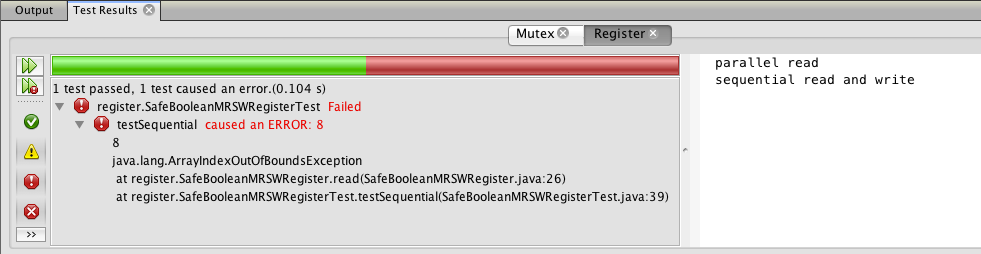
\includegraphics[width=13cm]{SafeBooleanMRSW00.png}
  \caption{First type of failure}
  \label{fig:SafeBooleanMRSW00}
\end{figure}
\par
\begin{figure}[h]
  \centering
  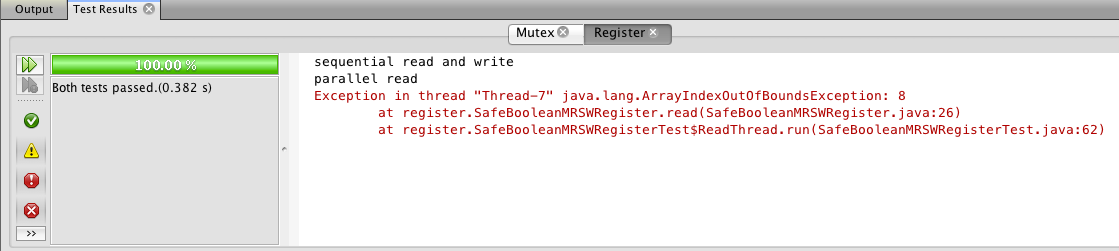
\includegraphics[width=13cm]{SafeBooleanMRSW01.png}
  \caption{Second type of failure}
  \label{fig:SafeBooleanMRSW01}
\end{figure}
\par
So, the way to fix this problem was to make sure that in each test case
the threads ids are reset calling the static method $ThreadID.reset()$. With
this hack, the tests passed (See figure \ref{fig:SafeBooleanMRSW02}).
\par
\begin{figure}[h]
  \centering
  \includegraphics[width=13cm]{SafeBooleanMRSW02.png}
  \caption{Output after fix}
  \label{fig:SafeBooleanMRSW02}
\end{figure}
\par
\begin{figure}[h]
  \centering
  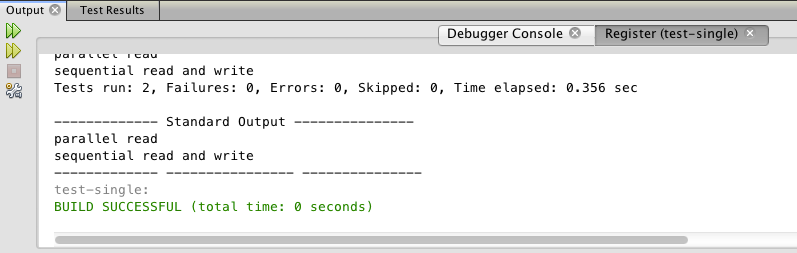
\includegraphics[width=13cm]{SafeBooleanMRSW03.png}
  \caption{Output after fix of threadIds}
  \label{fig:SafeBooleanMRSW03}
\end{figure}
\par
% ------------------------------------------------------------------------------------ %
\subsection{Interpretation}
\par
In this experiment we saw a way of implementing Safe Multi-Reader Single-Writer
registers. These registers were able of storing boolean values.
\par
Unfortunately, none of the test cases excersice the case where we have
concurrent writes and reads. Hence, this experiment only excersiced one of the
two rules of a safe register.
% ------------------------------------------------------------------------------------ %

\section{\textbf{RegMRSWRegisterTest}}

\subsection{Particular Case (problem)}
The problem we face here is that of building a regular multi-valued
multiple-reader single-writer register; out of simpler constructions,
like the rest of chapter 4. 

\subsection{Solution}
The solution, though supporting multi-values (integers), is bounded in
the range of values. We use as primitive blocks regular boolean
multiple-reader single-writer registers; and create an array of them
(as many as values in supported range), and use it to represent
numbers in unary way. That is, each position on the array that is set
to true represents the number corresponding to that position (the
index itself is the number). \\

Initially the boolean array is initialized to zero value, indicated by
having true the cell at index 0. The write method of value \C{x} sets
to true array position \C{x}, and updates to false the lower value
positions (so it updates from right to left). In order to guarantee
the regular property, the read method operates on the opposite
direction: it goes from left to right, starting at zero position, and
returns the first position whose value is true (an invariant of the
array should be that there is at least one cell in with true
value). The code from the book is presented below, for further
reference (the range of values picked
by the book's authors was that of byte Java type): \\

\newpage
\begin{lstlisting}[style=numbers]
public class RegMRSWRegister implements Register<Byte> {
  private static int RANGE = Byte.MAX_VALUE - Byte.MIN_VALUE + 1;
  // regular boolean mult-reader single-writer register
  boolean[] r_bit = new boolean[RANGE]; 
  public RegMRSWRegister(int capacity) {
    r_bit[0] = true; // least value
  }
  public void write(Byte x) {
    r_bit[x] = true;
    for (int i = x - 1; i >= 0; i--)
      r_bit[i] = false;
  }
  public Byte read() {
    for (int i = 0; i < RANGE; i++)
      if (r_bit[i]) {
        return (byte)i;
      }
    return -1;  // never reached
  }
}
\end{lstlisting}
\hfill

\subsection{Experiment Description}
The test program \C{RegMRSWRegisterTest} includes the following individual
test cases (which is pretty much the same thing as test
\C{AtomicMRMWRegisterTest}):

\begin{itemize}
  \item \C{testSequential}: calls \C{write} method first with a value
    of 11, then calls \C{read} method expecting read 11. A single
    thread is used (main thread).
  \item \C{testParallel}: calls twice method \C{write}, putting first
    11 then 22 value. Then proceeds to create 8 reader threads, which
    expect all to read 22. 
\end{itemize}

\subsection{Observations and Interpretations}
Just like \C{AtomicMRMWRegisterTest}, this does not exhibit any issue
on two nor in 24 core machines. Again, part of that reason is that the
test is not really interlacing writes with reads. A sample successful
execution is shown below: \\

\begin{verbatim}
$ junit register.RegMRSWRegisterTest
.sequential read and write
.parallel read

Time: 0.004

OK (2 tests)
\end{verbatim}
\hfill


% -------------------------------------------------------- %
% Regular Boolean MRSW Register Lock
% by: Isai Barajas Cicourel


% -------------------------------------------------------- %
% Document Start

\section{\textbf{Regular Boolean MRSW Register}}


% -------------------------------------------------------- %
% Particular Caes

\subsection{Particular Case}
\par
A register, is an object that encapsulates a value that can be observed by a \textit{read()} method and modified by a \textit{write()} method
\par
For Boolean registers, the only difference between safe and regular arises when the newly written value $x$ is the same as the old. A regular register can only return $x$, while a safe register may return either Boolean value.
\par


% -------------------------------------------------------- %
% Solution Information

\subsection{Solution}
\par
A register that implements the \textit{Register<Boolean>} interface is called a Boolean register (we sometimes use 1 and 0 as synonyms for true and false).
This register uses the \textit{ThreadLocal} Java java.lang package, which provides thread-local variables. These variables differ from their normal counterparts in that each thread that accesses one (via its get or set method) has its own, independently initialized copy of the variable. \textit{ThreadLocal} instances are typically private static fields in classes that wish to associate state with a thread
\par
\begin{lstlisting}[frame=single,breaklines=true]
public class RegBooleanMRSWRegister 
implements Register<Boolean> {
  ThreadLocal<Boolean> last;
  private boolean s_value;
  RegBooleanMRSWRegister(int capacity) {
    this.last = new ThreadLocal<Boolean>() {
      protected Boolean initialValue() { return false; };
    };
  }
  public void write(Boolean x) {
    if (x != last.get()) {  // if new value different ...
      last.set(x);          // remember new value
      s_value =x;           // update register
    }
  }
  public Boolean read() {
    return s_value;
  }
}
\end{lstlisting}

% -------------------------------------------------------- %
% Experiment

\subsection{Experiment Description} 
\par
The test creates $8$ threads that reads the value of a register. All threads have to be able to read the current value of the register despite the previous value is contrary to the current one.
The expected result is must be a $1$ or true value.
\par

% -------------------------------------------------------- %
% Results

\subsection{Observations and Interpretations}
\par
The tests executed as expected and no errors where found.


% -------------------------------------------------------- %
% SeqSnapshot
% by: Isai Barajas Cicourel


% -------------------------------------------------------- %
% Document Start

\section{\textbf{Sequential Snapshot}}


% -------------------------------------------------------- %
% Particular Caes

\subsection{Particular Case}
\par
In order to read multiple register values atomically we use an atomic snapshot.
An atomic snapshot constructs an instantaneous view of an array of atomic registers. We construct a wait-free snapshot, meaning that a thread can take an instantaneous snapshot of memory without delaying any other thread.
\par


% -------------------------------------------------------- %
% Solution Information

\subsection{Solution}
\par
Each thread repeatedly calls \textit{collect()}, and returns as soon as it detects a clean double collect (one in which both sets of timestamps were identical). This construction always returns correct values. The \textit{update()} calls are wait-free, but \textit{scan()} is not because any call can be repeatedly interrupted by \textit{update()}, and may run forever without completing. It is however obstruction-free, since a \textit{scan()} completes if it runs by itself for long enough.
\begin{lstlisting}[frame=single,breaklines=true]
public class SeqSnapshot<T> implements Snapshot<T> {
  private T[] a_value;
  public SeqSnapshot(int capacity, T init) {
    a_value = (T[])new Object[capacity];
    for (int i = 0; i < a_value.length; i++) {
      a_value[i] = init;
    }
  }
  public synchronized void update(T v) {
    a_value[ThreadID.get()] = v;
  }
  public synchronized T[] scan() {
    T[] result = (T[]) new Object[a_value.length];
    for (int i = 0; i < a_value.length; i++)
      result[i] = a_value[i];
    return result;
  }
}
\end{lstlisting}
\par


% -------------------------------------------------------- %
% Experiment

\subsection{Experiment Description} 
\par
The test creates $2$ threads that write the register twice with the the values \textit{FIRST} and \textit{SECOND} and later parallel reads the values.
\par

% -------------------------------------------------------- %
% Results

\subsection{Observations and Interpretations}

\par
When executing the test the test fails on the parallel part due to a index out of bound exception.
\begin{lstlisting}[frame=single,breaklines=true]
Testcase: testSequential(register.SeqSnapshotTest):	Caused an ERROR
2
java.lang.ArrayIndexOutOfBoundsException: 2
	at register.SeqSnapshot.update(SeqSnapshot.java:26)
	at register.SeqSnapshotTest.testSequential(SeqSnapshotTest.java:40)
\end{lstlisting}


% -------------------------------------------------------- %
% Results

\subsection{Proposed changes to fix the problem}

\par
By resetting the thread id at the beginning of the test the id is guarantee to be the experted while doing the parallel test.
\begin{lstlisting}[frame=single,breaklines=true]
  class MyThread extends Thread {
    public void run() {
      ThreadID.reset();
      instance.update(FIRST);
      instance.update(SECOND);
      Object[] a = instance.scan();
      for (Object x : a) {
        Integer i = (Integer) x;
        int me = ThreadID.get();
        for (int j = 0; j < THREADS; j++) {
          results[me][j] = (Integer)a[j];
        }
      }
    }
  }
\end{lstlisting}
Once the change is made the execution works fine on every equipment used.
\begin{lstlisting}[frame=single,breaklines=true]
Tests run: 2, Failures: 0, Errors: 0, Skipped: 0, Time elapsed: 0.097 sec

------------- Standard Output ---------------
sequential
parallel
------------- ---------------- ---------------
test-single:
BUILD SUCCESSFUL (total time: 0 seconds)
\end{lstlisting}


% -------------------------------------------------------- %
% Why?

\subsection{Proposed solution}
\par
Once the ThreadID is reset before changing from the sequential to the parallel test the execution never fails, since the out of bound happens due to the id being incremental.


\section{\textbf{Atomic MRSW Register}}
% -------------------------------------------------------------------------------- %
\subsection{Particular Case}
\par
The characteristics of this type of register are:
\begin{itemize}
\item It should never happen that $R^{i} \rightarrow W^{i}$
\item It should never happen that for any ${j}$, ${W^{i} \rightarrow W^{j} \rightarrow R^{j}}$
\item If ${R^{i} \rightarrow R^{j}}$ then ${i \leq j}$
\end{itemize}
The book proposes to do this by using multiple SRSW registers.
% -------------------------------------------------------------------------------- %
\subsection{Solution}
The algorithm then requires a 2 dimensional table. When a writer decides to
update the register, it has to update the values in cells $A[i][i]$, where $i$
is the thread id. Apart from writing the value, it has to also update the cell
with a timestamp. 
\par
In the other hand, when a reader wants to read from the register, it checks the
timestamp of the cell $A[i][i]$. After that, it has to check other cells in the
same column (ie, cells $A[x][i]$) to see if there has been an update in between.
That is done by comparing the timestamps. If there is a newer timestamp, the
reader has then to update all cells in its row (ie $A[i][x]$). This is the way
to indicate subsequent readers which version of the value has the previous
reader retrieved.
\par
It is easy to see that the first property is satisfied because there is no way
to read a future value. In order to read a value, this value has to be written
before.
\par
The second property is also satisfied because when a reader reads the value, it
reads the one with the most recent timestamp by scaning the timestamps in its
corresponding column. This reader also helps subsequent readers by updating all
cells in its row. Forcing property 3 to be satisfied as well.
\par
% -------------------------------------------------------------------------------- %
\subsection{Experiment Description}
\par 
The two test cases presented demonstrates the same as previous examples so we
will not describe the experiment further. 
\par
These are the details of the system we used to run the experiments:
\begin{itemize}
\item Processor: Intel Core i5 @2.5 GHz. 2 Cores.
\item L2 Cache per Core: 256 KB
\item L3 Cache: 3 MB
\item System Memory: 16 GB
\end{itemize}
% -------------------------------------------------------------------------------- %
\subsection{Sample Results}
As in previous examples, we identified that the test fails from time to time.
Figure \ref{fig:AtomicMRSW00} shows the output when the failure is seen.
\par
\par
\begin{figure}[h]
  \centering
  \includegraphics[width=13cm]{AtomicMRSW00.png}
  \caption{First type of failure}
  \label{fig:AtomicMRSW00}
\end{figure}
\par
Again, the fix for these failures was to reset the thread ids.
\par
\begin{figure}[h]
  \centering
  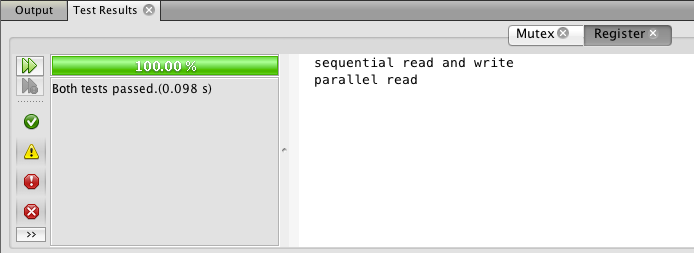
\includegraphics[width=13cm]{AtomicMRSW01.png}
  \caption{Output after fix}
  \label{fig:AtomicMRSW01}
\end{figure}
\par
\begin{figure}[h]
  \centering
  \includegraphics[width=13cm]{AtomicMRSW02.png}
  \caption{Output after fix of threadIds}
  \label{fig:AtomicMRSW03}
\end{figure}
\par
% -------------------------------------------------------------------------------- %
\subsection{Interpretation}
\par
In this experiment we observed a way of implementing MRSW registers. We saw
that, at least in the processor we used, the algorithm seems to work correctly.
\par
It would have been great, though, to also have test cases that demonstrate that this
particular register satisfies property 3 which is the one that makes it
different from the Safe version.
% -------------------------------------------------------------------------------- %

\section{\textbf{AtomicMRMWRegisterTest}}

\subsection{Particular Case (problem)}
The problem we are trying to solve here, is that of implementing an
atomic multi-valued \footnote{As opposed to boolean values, which have
only a couple of values; while multi-valued can range over a big set,
like integers.}
multiple-reader multiple-writer register. Let us 
briefly recall that atomic registers are the most powerful ones, when
compared with the 
other two categories: safe and regular. Informally, atomic registers
behave like one would expect when reads overlap writes: the reads
always ``see'' the last written value; while regular registers allows
to see either previous or latest value. Finally ``safe'' registers
allow reads to see any value (not safe at all then!). 

\subsection{Solution}
The solution from the book uses as primitive blocks the atomic
multi-valued multi-reader single-writer registers; we build an array of them whose
size equals the number of threads we want to support (assuming number
of writers is same as readers). When a given thread \C{A} wants to
write a value, it needs to read all the values on the array and writes
to its own cell an stamped value that is bigger than any one
observed. When same thread wants to read a value, it reads again whole
array and returns the one with biggest stamped value (resolving ties
with thread ids). This is essentially the same as Lamport's Bakery
algorithm from mutual exclusion chapter; the code is small enough to
fit here, so there it goes for reference: \\

\newpage
\begin{lstlisting}[style=numbers]
public class AtomicMRMWRegister<T> implements Register<T>{
  // array of multi-reader single-writer registers
  private StampedValue<T>[] a_table; 
  public AtomicMRMWRegister(int capacity, T init) {
    a_table = (StampedValue<T>[]) new StampedValue[capacity];
    StampedValue<T> value = new StampedValue<T>(init);
    for (int j = 0; j < a_table.length; j++) {
      a_table[j] = value;
    }
  }
  public void write(T value) {
    int me = ThreadID.get();
    StampedValue<T> max = StampedValue.MIN_VALUE;
    for (int i = 0; i < a_table.length; i++) {
      max = StampedValue.max(max, a_table[i]);
    }
    a_table[me] = new StampedValue<T>(max.stamp + 1, value);
  }
  public T read() {
    StampedValue<T> max = StampedValue.MIN_VALUE;
    for (int i = 0; i < a_table.length; i++) {
      max = StampedValue.max(max, a_table[i]);
    }
    return max.value;
  }
}
\end{lstlisting}

\subsection{Experiment Description}
The test program AtomicMRMWRegisterTest includes the following individual
test cases: 

\begin{itemize}
  \item \C{testSequential}: calls \C{write} method first with a value
    of 11, then calls \C{read} method expecting read 11. A single
    thread is used (main thread).
  \item \C{testParallel}: calls twice method \C{write}, putting first
    11 then 22 value. Then proceeds to create 8 reader threads, which
    expect all to read 22. This test is not really exercising
    multi-write capability of the register.
    sequentially.
\end{itemize}

\subsection{Observations and Interpretations}
The test performs well on 2 and 24 core machines, without any race
conditions nor abnormal behaviors. This partly because, the test is
not really exercising the multi-write capability, nor the interlacing
of writes and reads. We believe the authors just copied paste a
previous test (probably one that just cared about single reader and
multiple writers), and forgot to update. Due time constraints we did
not modify the test to exercise those missing features; a sample
execution is shown below: \\\\

\begin{verbatim}
$ junit register.AtomicMRMWRegisterTest
.sequential read and write
.parallel read

Time: 0.004

OK (2 tests)
\end{verbatim}
\hfill

\newpage
\section{\textbf{SimpleSnapshotTest}}

\subsection{Particular Case (problem)}
The problem we want to solve is that of atomic snapshots: we want to
read atomically a set of registers. For this problem we assume the
registers are themselves atomic, and that each one supports
multiple-readers but just one writer. The problem is better defined in 
terms of the Java interface we want to implement: \\

\begin{lstlisting}[style=nonumbers]
public interface Snapshot<T> {
  public void update(T v);
  public T[] scan();
}
\end{lstlisting}
\hfill

While the method \C{update} allows each thread to modify its own
register (single-writer), the \C{scan} method allows any thread to
read all the registers as a single atomic operation
(multiple-readers). Ideally, we would like to have a wait-free
implementation of these two methods.

\subsection{Solution}
The solution presented in the book is a natural evolution to the
sequential implementation (which uses \C{synchronized} methods for
both \C{update} and \C{scan} methods). The solution is called
\C{SimpleSnapshot} and it uses stamped values for the \C{update}
method; there is no need to seek for the maximum, just to increase the
current stamp per thread (each thread only writes to its own
register). This makes the \C{update} method wait-free, which is the
ideal (it was not very hard to achieve indeed, given the single-writer
restriction). \\

For the \C{scan} method we call an auxiliary function \C{collect},
which represents a non atomic read of all the registers (which are
copied into a new array and returned); if two
consecutive \C{collect} calls return same values, it means that between
those two calls there were no writes. When we reach that condition, we
return the array of values; otherwise we repeat the iteration. Please
note that \C{scan} method is not wait-free (we do not know how many
times we will need to iterate), but at least is
obstruction-free (we are not blocking other threads from trying their
own \C{scan} calls). \\

The main parts of the code are presented below for reference: \\

\begin{lstlisting}[style=numbers]
public class SimpleSnapshot<T> implements Snapshot<T> {
  // array of atomic MRSW registers
  private StampedValue<T>[] a_table;  
  ...
  public void update(T value) {
    int me = ThreadID.get();
    StampedValue<T> oldValue = a_table[me];
    StampedValue<T> newValue =
        new StampedValue<T>((oldValue.stamp)+1, value);
    a_table[me] = newValue;
  }
  private StampedValue<T>[] collect() {
    StampedValue<T>[] copy = (StampedValue<T>[]) new StampedValue[a_table.length];
    for (int j = 0; j < a_table.length; j++)
      copy[j] = a_table[j];
    return copy;
  }
  public T[] scan() {
    StampedValue<T>[] oldCopy, newCopy;
    oldCopy = collect();
    collect: while (true) {
      newCopy = collect();
      if (! Arrays.equals(oldCopy, newCopy)) {
        oldCopy = newCopy;
        continue collect;
      }
      // clean collect
      T[] result = (T[]) new Object[a_table.length];
      for (int j = 0; j < a_table.length; j++)
        result[j] = newCopy[j].value;
      return result;
    }
  }
}
\end{lstlisting}
\hfill

\subsection{Experiment Description}

The test program \C{SimpleSnapshotTest} consists of two individual
test cases: 

\begin{itemize}
  \item \C{testSequential}: with a single thread we update its value
    first (11), and then obtain an snapshot (\C{scan}); expectation is
    to have a single value in array (the one we wrote).
  \item \C{testParallel}: we create a couple of threads, and each one
    writes its own register twice (first putting 11, then 22). Then
    each thread proceeds to call \C{scan} method and saves its own
    returned values into a global results table. At the end of test,
    main thread check that both threads got the same results (which
    should be a two element array, both with value 22). 
\end{itemize}

\subsection{Observations and Interpretations}
The test runs fine, both in 2 and 24 core machines; sample output
below: \\

\begin{verbatim}
$ junit register.SimpleSnapshotTest
.sequential
.parallel

Time: 0.002

OK (2 tests)
\end{verbatim}
\hfill


\section{\textbf{Wait-Free Snapshots}}
% ---------------------------------------------------------------------------- %
\subsection{Particular Case}
\par
In this experiment we are dealing with the problem of creating an algorithm to
create a Snapshot of a set of Register in such a way that the algorithm
guarantees a Wait-Free operation.
\par
% ---------------------------------------------------------------------------- %
\subsection{Solution}
\par
The purpose of a Wait-Free snapshot is to overcome the problems of the Simple
snapshot presented before. Let us remember that such snapshot executes successive
collect() operations. Once it achieves a \textit{clean double collect}, it
returns the snapshot. Otherwise, it uses the following idea:
\par
When a double collect fails, it is because a update interfered. That means that
the updater could take a snapshot right before its update and other threads
could use it as their snapshot too. 
\par
Since this algorithm is a bit more complex, let us explain in more detail how
the implementation works.
\par
\hfill
\begin{lstlisting}[style=numbers]
  public WFSnapshot(int capacity, T init) {
    a_table = (StampedSnap<T>[]) new StampedSnap[capacity];
    for (int i = 0; i < a_table.length; i++) {
      a_table[i] = new StampedSnap<T>(init);
    }   
  }
\end{lstlisting}
\hfill
\par
Firstly, the algorithm uses an array to store the information.
The size of the array is, in this case, $n$, where $n$ is the number of
threads. The way in which this array is constructed is as an array of
\textit{StampedSnap}s. A StampedSnap is internally an array whose elements are
of type \textit{T}. A StampedSnap is a subclass of StampedValue which has 3
fields:
\par
\begin{itemize}
\item \textit{stamp}, which is a counter
\item \textit{owner}, which contains the thread id
\item \textit{value}, the actual value in the register
\end{itemize}
\par
Now let us look at an auxiliar operation which is \textit{collect()}. This
operation returns a copy of the array. Observe that the method creates a new
array of StampedSnap values and then iterates the existing array to copy each element.
\par
\hfill
\begin{lstlisting}[style=numbers]
  private StampedSnap<T>[] collect() {
    StampedSnap<T>[] copy = (StampedSnap<T>[]) new StampedSnap[a_table.length];
    for (int j = 0; j < a_table.length; j++)
      copy[j] = a_table[j];
    return copy;
  }
\end{lstlisting}
\hfill
\par
The next method to understand is \textit{scan()}. The method first creates a
backup or an old copy of the array. Then it takes a second collect. It then
compares both copies. If both copies are equal, then it means that we have a
double clean collect. And the result of the scan operation is any of the copies
just as in the Sequential Snapshot case.
\par
On the other hand, if the copies are different, then there are two cases. For
this, we have a counter that indicates how many times, the copies have been
compared and found different. If it is the first time, then we take another
collect. If in the second collect, the copies are equal, then we fall in the
case described in the previous paragraph. If the copies are different again,
then it means that we can take the old copy as a result of the scan. 
\par
The justification of this is that if a thread A sees a thread B move twice while
it is performing repeated collects, then B executed a complete \textit{update()}
call within the interval of A's scan, and so it is correct for A to use B's
snapshot.
\par
\hfill
\begin{lstlisting}[style=numbers]
  public T[] scan() {
    StampedSnap<T>[] oldCopy;
    StampedSnap<T>[] newCopy;
    boolean[] moved = new boolean[a_table.length];
    oldCopy = collect();
    collect: while (true) {
      newCopy = collect();
      for (int j = 0; j < a_table.length; j++) {
        // did any thread move?
        if (oldCopy[j].stamp != newCopy[j].stamp) {
          if (moved[j]) {       // second move
            return oldCopy[j].snap;
          } else {
            moved[j] = true;
            oldCopy = newCopy;
            continue collect;
          }   
        }   
      }   
      // clean collect
      T[] result = (T[]) new Object[a_table.length];
      for (int j = 0; j < a_table.length; j++)
        result[j] = newCopy[j].value;
      return result;
    }   
  }
\end{lstlisting}
\hfill
\par
Finally, we have the \textit{update()} operation which simply updates the
register with the new stamp.
\par
\hfill
\begin{lstlisting}[style=numbers]
  public void update(T value) {
    int me = ThreadID.get();
    T[] snap = this.scan();
    StampedSnap<T> oldValue = a_table[me];
    StampedSnap<T> newValue =
      new StampedSnap<T>(oldValue.stamp+1, value, snap);
    a_table[me] = newValue;
  }
\end{lstlisting}
\hfill
% ---------------------------------------------------------------------------- %
\subsection{Experiment Description}
\par
In this experiment, the test looks a bit different. Let us explain how. In this
case we have two experiments:
\par
\begin{enumerate}
\item testSequential. We spawn a new thread that updates the register with a
value of \textit{FIRST} and right after that, it scans the value of the
register. The expected result is that this read retrieves the value of
\textit{FIRST}
\item testParallel. We spawn \textit{THREADS} number of threads (in our case it
is $2$). Each of them will first update its register with a value of
\textit{FIRST} and then with a value of \textit{SECOND}. Each thread then
updates a position in a matrix of size \textit{THREADS}$x$\textit{THREADS} with
the result of doing a $scan()$ operation. At the end we compare consecutive rows
in the matrix. The comparison is done entry by entry and we should see that for
some entries the first entry is greater and for some others it is smaller than
the second. What we must see is that all entries are equal and we allow the
first to sometimes be either greater or smaller than the second one.
\end{enumerate}
% ---------------------------------------------------------------------------- %
\subsection{Sample Results}
\par
For this test, we saw that in every try, both test cases passed. Here is the
output:
\par
\begin{verbatim}
[oraadm@gdlaa008 Register]$ junit register.WFSnapshotTest
.sequential
.parallel

Time: 0.003

OK (2 tests)
\end{verbatim}
\par
% ---------------------------------------------------------------------------- %
\subsection{Interpretation}
% ---------------------------------------------------------------------------- %
In this experiment we were able to observe how a Wait-Free Snapshot can be
constructed based on the idea of \textit{clean double collects} and on the idea
of using the updater's collect when the clean double collect method fails.

% --------------------------- %
% Foundations End
% --------------------------- %

% --------------------------- %
% ch 07 Spin Locks Start
% --------------------------- %
\chapter{Spin Locks and Contention}
../../zava/Multiprocessor//SpinLocks.tex
../../zava/Multiprocessor//TASLockTest.tex
../../dario/Multiprocessor/TTASLockTest.tex
../../dario/Multiprocessor/BackoffLockTest.tex
\section{\textbf{CLH Queue Lock}}
%%%%%%%%%%%%%%%%%%%%%%%%%%%%%%%%%%
\subsection{Particular Case}
\par
Using queue locks solve two problems that appear in simpler locking protocols.
Firstly, by using a queue, cache-coherence traffic is reduced because each
thread spin on a different memory location; and secondly, by using a queue,
threads can know whether their turn has come by inspecting the status of their
predecesor in the queue.
\par
The particular case that we want to study in this experiment is \textit{How can
we implemente a space efficient Queue Lock?}
\par
%%%%%%%%%%%%%%%%%%%%%%%%%%%%%%%%%%
\subsection{Solution}
\par
One solution for this problem is given by the CLHLock protocol. The algorithm
that implement this protocol need two fields local to the thread: A pointer to
the current node and a pointer to the previous node. The queue is constructed by
having the pointer \textit{previous} pointing to the previous node's
\textit{current} field. This field contains a boolean value which is false when
the thread releases the lock. When this is the case, the next thread is allowed
to acquire the lock. 
\par
%%%%%%%%%%%%%%%%%%%%%%%%%%%%%%%%%%
\subsection{Experiment Description}
\par
To demonstrate that this implementation works, the test that was provided does
the following:
\begin{enumerate}
\item Initiate a shared counter with a value of $0$
\item Start $8$ threads
\item Each thread has to increment the counter by one $1024$ times
\item At the end, the counter must hold a value of $8*1024$
\end{enumerate}
\par
%%%%%%%%%%%%%%%%%%%%%%%%%%%%%%%%%%
\subsection{Sample Results}
\par
In this case, we found that in our 24-cores machine, the test hung. To make it
work, we had to make the \textit{locked} variable in the 
\par
\hfill
\begin{verbatim}
[oraadm@gdlaa008 Spin]$ junit spin.CLHLockTest 
[8] Leaving critical zone
[9] Entering critical zone
[9] Leaving critical zone
[8] Entering critical zone
[8] Leaving critical zone
[9] Entering critical zone
[9] Leaving critical zone
[8] Entering critical zone
[9] Entering critical zone
...
[9] Leaving critical zone
[8] Entering critical zone
[9] Entering critical zone
[8] Leaving critical zone
[8] Entering critical zone
[8] Leaving critical zone

Time: 0.755

OK (1 test)
\end{verbatim}
\hfill
\par
%%%%%%%%%%%%%%%%%%%%%%%%%%%%%%%%%%
\subsection{Interpretation}
It was shown that the algorithm seems to work and allows synchronization of
Multiple threads trying to access a shared variable.
\par
One important thing about this algorith is that threads spin checking for
different memory addresses which avoids invalidation of cached copies. Another
important advantage is that it requieres a limited number of memory and also
provides first-in-first-out fairness. 
\par
The case were this algorithm is not good is when, in a NUMA architecture, the
\textit{previous} pointer points to a remote location. In that case, the
performance of the algorithm degradates.

\section{\textbf{MCSLockTest}}

\subsection{Particular Case (problem)}
The problem is still how to build scalable spinning locks, and in
particular, how to overcome the limitations from the backoff
approaches. The queue-based approach introduced both \C{ALock} and
\C{CLHLock}, the first is space inefficient and the second overcomes
such limitation at the expense of not being suitable for cache-less
NUMA architecture.

\subsection{Solution}
The solution or rather alternative to \C{CLHLock} approach is called
\C{MCSLock}; and that is the algorithm tested in this section. Just
like the \C{CLHLock} approach, the lock is modeled with a linked
list of QNode objects, where each one represents either a lock holder
or a thread waiting to acquire the lock; the difference though, is
that the list is explicit, not virtual \footnote{The author introduces
  the term ``virtual'', when describing \C{CLHLock} because the
list is implicit: each thread refers to its predecessor through a
thread-local \C{pred} variable.}. On the \C{MCSLock} approach, instead of
embedding the list in thread-local variables, it is placed in the
globally accessible QNode objects.

The \C{MCSLock} code is presented below for further reference: \\

\begin{lstlisting}[style=numbers]
public class MCSLock implements Lock {
  AtomicReference<QNode> queue;
  ThreadLocal<QNode> myNode;
  public MCSLock() {
    queue = new AtomicReference<QNode>(null);
    // initialize thread-local variable
    myNode = new ThreadLocal<QNode>() {
      protected QNode initialValue() {
        return new QNode();
      }
    };
  }
  public void lock() {
    QNode qnode = myNode.get();
    QNode pred = queue.getAndSet(qnode);
    if (pred != null) {
      qnode.locked = true;
      pred.next = qnode;
      while (qnode.locked) {}     // spin
    }
  }
  public void unlock() {
    QNode qnode = myNode.get();
    if (qnode.next == null) {
      if (queue.compareAndSet(qnode, null))
        return;
      while (qnode.next == null) {} // spin
    }
    qnode.next.locked = false;
    qnode.next = null;
  }
  ...
  static class QNode {     // Queue node inner class
    boolean locked = false;
    QNode   next = null;
  }
}
\end{lstlisting}
\hfill

This \C{MCSLock} solution is not a perfect replacement for
\C{CLHLock}: on one side it has same advantages than \C{CLHLock}, in
particular, the property that each lock release invalidates only the
successor's cache entry, with the plus that it is better suited to
cache-less NUMA architectures because each thread controls the
location on which it spins. The space complexity is the same as
\C{CLHLock}, \bigO{L + n}, as the nodes can be recycled. \\

On the other side, the disadvantages of \C{MCSLock} algorithm is that
releasing a lock requires spinning; and that it requires more reads,
writes, and compareAndSet() calls than the \C{CLHLock} algorithm.

\subsection{Experiment Description}

The test is exactly the same as that of \C{BackoffLockTest}: 8 threads
try to increment 1024 times a shared counter, and they do that
concurrently. At the end the counter shall have $8 * 1024$ as final
value. 

\subsection{Observations and Interpretations}
The test works fine in two-cores, but in 24 cores it hangs time to
time; below a sample thread dump captured when hanging occurred (after
trying the test a bit more than 300 times):

\begin{verbatim}
Full thread dump OpenJDK 64-Bit Server VM (23.7-b01 mixed mode):

"Thread-7" prio=10 tid=0x00007f3c4c0e0000 nid=0x6aaa runnable [0x00007f3bf6e4c000]
   java.lang.Thread.State: RUNNABLE
	at spin.MCSLock.lock(MCSLock.java:41)
	at spin.MCSLockTest$MyThread.run(MCSLockTest.java:52)

"Thread-6" prio=10 tid=0x00007f3c4c0de000 nid=0x6aa9 runnable [0x00007f3bf6f4d000]
   java.lang.Thread.State: RUNNABLE
	at spin.MCSLock.lock(MCSLock.java:41)
	at spin.MCSLockTest$MyThread.run(MCSLockTest.java:52)

"Thread-5" prio=10 tid=0x00007f3c4c0dc000 nid=0x6aa8 runnable [0x00007f3bf704e000]
   java.lang.Thread.State: RUNNABLE
	at spin.MCSLock.lock(MCSLock.java:41)
	at spin.MCSLockTest$MyThread.run(MCSLockTest.java:52)

"Thread-4" prio=10 tid=0x00007f3c4c0da000 nid=0x6aa7 runnable [0x00007f3bf714f000]
   java.lang.Thread.State: RUNNABLE
	at spin.MCSLock.lock(MCSLock.java:41)
	at spin.MCSLockTest$MyThread.run(MCSLockTest.java:52)

"Thread-3" prio=10 tid=0x00007f3c4c0d7000 nid=0x6aa6 runnable [0x00007f3bf7250000]
   java.lang.Thread.State: RUNNABLE
	at spin.MCSLock.lock(MCSLock.java:41)
	at spin.MCSLockTest$MyThread.run(MCSLockTest.java:52)

"Thread-2" prio=10 tid=0x00007f3c4c0d5800 nid=0x6aa5 runnable [0x00007f3bf7351000]
   java.lang.Thread.State: RUNNABLE
	at spin.MCSLock.lock(MCSLock.java:41)
	at spin.MCSLockTest$MyThread.run(MCSLockTest.java:52)

"Thread-1" prio=10 tid=0x00007f3c4c0d4000 nid=0x6aa4 runnable [0x00007f3bf7452000]
   java.lang.Thread.State: RUNNABLE
	at spin.MCSLock.lock(MCSLock.java:41)
	at spin.MCSLockTest$MyThread.run(MCSLockTest.java:52)

"Thread-0" prio=10 tid=0x00007f3c4c0d8800 nid=0x6aa3 runnable [0x00007f3bf7553000]
   java.lang.Thread.State: RUNNABLE
	at spin.MCSLock.lock(MCSLock.java:41)
	at spin.MCSLockTest$MyThread.run(MCSLockTest.java:52)
...
"main" prio=10 tid=0x0000000000c8a800 nid=0x6a79 in Object.wait() [0x00007f3c5ce0d000]
   java.lang.Thread.State: WAITING (on object monitor)
	at java.lang.Object.wait(Native Method)
	- waiting on <0x000000058386adc8> (a spin.MCSLockTest$MyThread)
	at java.lang.Thread.join(Thread.java:1260)
	- locked <0x000000058386adc8> (a spin.MCSLockTest$MyThread)
	at java.lang.Thread.join(Thread.java:1334)
	at spin.MCSLockTest.testParallel(MCSLockTest.java:43)
	at sun.reflect.NativeMethodAccessorImpl.invoke0(Native Method)
	at sun.reflect.NativeMethodAccessorImpl.invoke(NativeMethodAccessorImpl.java:57)
	at sun.reflect.DelegatingMethodAccessorImpl.invoke(DelegatingMethodAccessorImpl.java:43)
	at java.lang.reflect.Method.invoke(Method.java:606)
	at junit.framework.TestCase.runTest(TestCase.java:176)
	at junit.framework.TestCase.runBare(TestCase.java:141)
	at junit.framework.TestResult$1.protect(TestResult.java:122)
	at junit.framework.TestResult.runProtected(TestResult.java:142)
	at junit.framework.TestResult.run(TestResult.java:125)
	at junit.framework.TestCase.run(TestCase.java:129)
	at junit.framework.TestSuite.runTest(TestSuite.java:252)
	at junit.framework.TestSuite.run(TestSuite.java:247)
	at junit.textui.TestRunner.doRun(TestRunner.java:116)
	at junit.textui.TestRunner.start(TestRunner.java:183)
	at junit.textui.TestRunner.main(TestRunner.java:137)
\end{verbatim}
\hfill

From the above stacks, we can observe that the main thread hangs
because none of the launched 8 threads gets out of the spinning while
of \C{lock} method (line 41): \\

\begin{lstlisting}[style=numbers]
      while (qnode.locked) {}     // spin
\end{lstlisting}
\hfill

The reason of the above must be that the \C{locked} flag is not
declared as \C{volatite}; without such keyword, the JVM does not
guarantee any synchronization time limits between the \C{RAM} and the local
caches of each core. Thus, the hanging shall occur when the write made
by last thread to its local flag (\C{locked=false}, did not get
propagated to any other core for a while; we do now know when they
would get propagated, actually. \\

This is an interesting aspect of the \C{AtomicReference} class; while
it does cover the ``reference'' to a \C{QNode}, it does not
appear to affect the attributes of the object. Thus, changes to the
\C{queue} reference will be atomic indeed; but they would point to
attributes whose writes are not. \\

One may be tempted to think that the \C{volatile} keyword is only
applicable to the \C{locked} boolean flag; but even with that chance
the test may still hang. Below sample thread dump on the 24 cores
machine, after retrying test 1118 times: \\

\begin{verbatim}
Full thread dump OpenJDK 64-Bit Server VM (23.7-b01 mixed mode):

"Thread-7" prio=10 tid=0x00007f55b00ef800 nid=0x9e07 runnable [0x00007f555c6e8000]
   java.lang.Thread.State: RUNNABLE
	at spin.MCSLock.unlock(MCSLock.java:49)
	at spin.MCSLockTest$MyThread.run(MCSLockTest.java:56)

"Thread-6" prio=10 tid=0x00007f55b00ed800 nid=0x9e06 runnable [0x00007f555c7e9000]
   java.lang.Thread.State: RUNNABLE
	at spin.MCSLock.lock(MCSLock.java:41)
	at spin.MCSLockTest$MyThread.run(MCSLockTest.java:52)

  ...

"main" prio=10 tid=0x00000000018eb800 nid=0x9dd6 in Object.wait() [0x00007f55c2736000]
   java.lang.Thread.State: WAITING (on object monitor)
	at java.lang.Object.wait(Native Method)
	- waiting on <0x000000058386b910> (a spin.MCSLockTest$MyThread)
	at java.lang.Thread.join(Thread.java:1260)
	- locked <0x000000058386b910> (a spin.MCSLockTest$MyThread)
	at java.lang.Thread.join(Thread.java:1334)
	at spin.MCSLockTest.testParallel(MCSLockTest.java:43)
	at sun.reflect.NativeMethodAccessorImpl.invoke0(Native Method)
	at sun.reflect.NativeMethodAccessorImpl.invoke(NativeMethodAccessorImpl.java:57)
	at sun.reflect.DelegatingMethodAccessorImpl.invoke(DelegatingMethodAccessorImpl.java:43)
	at java.lang.reflect.Method.invoke(Method.java:606)
	at junit.framework.TestCase.runTest(TestCase.java:176)
	at junit.framework.TestCase.runBare(TestCase.java:141)
	at junit.framework.TestResult$1.protect(TestResult.java:122)
	at junit.framework.TestResult.runProtected(TestResult.java:142)
	at junit.framework.TestResult.run(TestResult.java:125)
	at junit.framework.TestCase.run(TestCase.java:129)
	at junit.framework.TestSuite.runTest(TestSuite.java:252)
	at junit.framework.TestSuite.run(TestSuite.java:247)
	at junit.textui.TestRunner.doRun(TestRunner.java:116)
	at junit.textui.TestRunner.start(TestRunner.java:183)
	at junit.textui.TestRunner.main(TestRunner.java:137)
\end{verbatim}
\hfill


In the above dump there are only hanging threads two; ``Thread-6'' is
waiting on the already seen spinning loop of \C{lock} method, which should no
longer be attributable to the lack of \C{volatile} attribute (we just
fixed that). This spinning loop of the ``Thread-6'' hanging thread
then, must be valid: the \C{locked} flag of the other thread has not
changed. \\

The new part is the other hanging thread ``Thread-7'', which is
waiting on the spinning loop of the \C{unlock} method: \\

\begin{lstlisting}[style=numbers]
      while (qnode.next == null) {} // spin
\end{lstlisting}
\hfill

We immediately notice same problem as with \C{locked} flag; the
\C{next} pointer also needs immediate propagation to main memory,
otherwise the threads will not detect then is being set to
null. Let us also note that the hanging due \C{next} variable,
triggers the hanging on the spinning loop for \C{lock} method; the
\C{locked} flag is volatile, so a write to it would propagate right
away and invalidate other's caches; but since the thread doing the
\C{unlock} never exits the loop, it can not perform such
write. Putting as volatile both attributes of class \C{Qnode} solves
this issue; we ran  the test 10,000 times without a hang. 

An interesting observation made while discussing this exercise on the
distribution list, was that the solution imposes a serialization,
after all; but that is correct. Let us remember that the queue is just
the internal implementation artifact of the high level lock
construction. And for this particular test, we are trying to solve the
mutual-exclusion problem for a counter; thus serialization is what we
want, indeed. \\

Even if serialization is required, there are several ways of achieving
it; some are more efficient at hardware level than others. The family
of solutions that \C{MCSLock} belongs to, tries to minimize traffic on
the core buses (as we only invalidate the cache of the core that owes
the modified variables \C{locked} / \C{next}).



% -------------------------------------------------------- %
% ALock
% by: Isai Barajas Cicourel


% -------------------------------------------------------- %
% Document Start

\section{\textbf{Array Lock}}


% -------------------------------------------------------- %
% Particular Caes

\subsection{Particular Case}
\par
The ALock, is a simple array-based queue lock. In a queue, each thread can learn if its turn has arrived by checking whether its predecessor has finished.
\par


% -------------------------------------------------------- %
% Solution Information

\subsection{Solution}
\par
The threads share an \textit{AtomicInteger} tail field, initially zero. To acquire the lock, each thread atomically increments tail. Call the resulting value the thread’s slot. The slot is used as an index into a Boolean flag array. If \textit{flag[j]} is true, then the thread with slot \textit{j} has permission to acquire the lock.
\begin{lstlisting}[frame=single,breaklines=true]
public class ALock implements Lock {
  // thread-local variable
  ThreadLocal<Integer> mySlotIndex = new ThreadLocal<Integer> (){
    protected Integer initialValue() {
      return 0;
    }
  };
  volatile AtomicInteger tail;
  volatile boolean[] flag;
  int size;
  /**
   * Constructor
   * @param capacity max number of array slots
   */
  public ALock(int capacity) {
    size = capacity;
    tail = new AtomicInteger(0);
    flag = new boolean[capacity];
    flag[0] = true;
  }
  public void lock() {
    int slot = tail.getAndIncrement() % size;
    mySlotIndex.set(slot);
    while (! flag[mySlotIndex.get()]) {}; // spin
  }
  public void unlock() {
    flag[mySlotIndex.get()] = false;
    flag[(mySlotIndex.get() + 1) % size] = true;
  }
  // any class implementing Lock must provide these methods
  public Condition newCondition() {
    throw new java.lang.UnsupportedOperationException();
  }
  public boolean tryLock(long time,
      TimeUnit unit)
      throws InterruptedException {
    throw new java.lang.UnsupportedOperationException();
  }
  public boolean tryLock() {
    throw new java.lang.UnsupportedOperationException();
  }
  public void lockInterruptibly() throws InterruptedException {
    throw new java.lang.UnsupportedOperationException();
  }
}
\end{lstlisting}
\par


% -------------------------------------------------------- %
% Experiment

\subsection{Experiment Description} 
\par
The test creates $8$ threads that need to be coordinate in order to increment a common counter. All threads have to cooperate to increase this counter from 0 to $1024$. Each of the threads will increase by one the counter $128$ times.
The expected result is that regardless of the order in which each thread executes the increment, at the end the counter must stay at $1024$.
If that is not the case, then it means that mutual exclusion did not work.
\par

% -------------------------------------------------------- %
% Results

\subsection{Observations and Interpretations}

\par
When executing the test values where lost from the queue.
\begin{lstlisting}[frame=single,breaklines=true]
1009
1010
1011
1013
1014
1015
\end{lstlisting}


% -------------------------------------------------------- %
% Results

\subsection{Proposed changes to fix the problem}

\par
By adding the volatile keyword in the ALock class the execution was fixed.
\begin{lstlisting}[frame=single,breaklines=true]
  volatile AtomicInteger tail;
  volatile boolean[] flag;
  int size;
\end{lstlisting}
Once the change is made the execution works fine on every equipment used.


% -------------------------------------------------------- %
% Why?

\subsection{Proposed solution}
\par
Apparently the AtomicInteger keyword is not guarantee that the values are propagated through the memory hierarchy and by making the value atomic the execution works.


% -------------------------------------------------------- %
% CompositeFastPath Lock
% by: Isai Barajas Cicourel


% -------------------------------------------------------- %
% Document Start

\section{\textbf{Composite Fast Path Lock}}


% -------------------------------------------------------- %
% Particular Caes

\subsection{Particular Case}
\par
In this experiment, we extend the \textit{CompositeLock} algorithm to encompass a fast path in which a solitary thread acquires an idle lock without acquiring a node and splicing it into the queue.
\par


% -------------------------------------------------------- %
% Solution Information

\subsection{Solution}
\par
We use a \textit{FASTPATH} flag to indicate that a thread has acquired the lock through the fast path. Because we need to manipulate this flag together with the tail field’s reference, we take a high-order bit from the tail field’s integer stamp. The private \textit{fastPathLock()} method checks whether the tail field’s stamp has a clear \textit{FASTPATH} flag and a null reference. If so, it tries to acquire the lock simply by applying \textit{compareAndSet()} to set the FASTPATH flag to true, ensuring that the reference remains null. An uncontended lock acquisition thus requires a single atomic operation. The \textit{fastPathLock()} method returns true if it succeeds, and false otherwise.
\par

% -------------------------------------------------------- %
% Experiment

\subsection{Experiment Description} 
\par
The test creates $2$ threads that need to be coordinate in order to increase a counter. All threads have to cooperate in order to increase the counter into the desire value, this lock implements a explicit lock that the test calls.
If that is not the case, an assertion fail will be raised.
\par


% -------------------------------------------------------- %
% Results

\subsection{Observations and Interpretations}

\par
The tests executed as expected and no errors where found. Since the \textit{CompositeFastPathLock} is used to acquire an explicit lock, the mutual exclusion is guarantee.

\begin{lstlisting}[frame=single,breaklines=true]
Tests run: 1, Failures: 0, Errors: 0, Skipped: 0, Time elapsed: 0.895 sec

test-single:
BUILD SUCCESSFUL (total time: 3 seconds)
\end{lstlisting}





% -------------------------------------------------------- %
% TO Lock
% by: Isai Barajas Cicourel


% -------------------------------------------------------- %
% Document Start

\section{\textbf{Time Out Lock}}


% -------------------------------------------------------- %
% Particular Caes

\subsection{Particular Case}
\par
In this experiment we consider the Java Lock interface which includes a \textit{tryLock()} method that allows the caller to specify a \textit{timeout} or maximum duration the caller is willing to wait to acquire the lock. The TOLock implements this mechanism in order to wait for a resource.
\par


% -------------------------------------------------------- %
% Solution Information

\subsection{Solution}
\par
The \textit{tryLock()} method creates a new QNode with a null pred field and appends it to the list as in the CLHLock class. If the lock was free, the thread enters the critical section. Otherwise, it spins waiting for its predecessor’s QNode’s pred field to change. If the predecessor thread times out, it sets the pred field to its own predecessor, and the thread spins instead on the new predecessor. 
\par
\begin{lstlisting}[frame=single,breaklines=true]
    while (System.nanoTime() - startTime < patience) {
      QNode predPred = pred.pred;
      if (predPred == AVAILABLE) {
        return true;
      } else if (predPred != null) {  // skip predecessors
        pred = predPred;
      }
    }
    // timed out; reclaim or abandon own node
    if (!tail.compareAndSet(qnode, pred))
      qnode.pred = pred;
\end{lstlisting}


% -------------------------------------------------------- %
% Experiment

\subsection{Experiment Description} 
\par
The test creates $8$ threads that need to be coordinate in order to increase a counter. All threads have to cooperate in order to increase the counter into the desire value, this lock implements a explicit lock that the test calls, but with the addition of a time out.
If that is not the case, an assertion fail will be raised.
\par

% -------------------------------------------------------- %
% Results

\subsection{Proposed changes to improve execution}

\par
By making volatile the QNode's in the TOLock class the execution finishes faster.
\begin{lstlisting}[frame=single,breaklines=true]
  volatile static QNode AVAILABLE = new QNode();
  volatile AtomicReference<QNode> tail;
  ThreadLocal<QNode> myNode;
\end{lstlisting}

% -------------------------------------------------------- %
% Results

\subsection{Observations and Interpretations}

\par
The tests executed as expected and no errors where found. But the time out generates some waiting depending on the number of cores the machine has.

\begin{lstlisting}[frame=single,breaklines=true]
Tests run: 2, Failures: 0, Errors: 0, Skipped: 0, Time elapsed: 22.551 sec

------------- Standard Output ---------------
locking
Created Threads
Started Threads
Finished Threads
timeout
timeouts: 8191
------------- ---------------- ---------------
test-single:
BUILD SUCCESSFUL (total time: 24 seconds)
\end{lstlisting}





\section{\textbf{CompositeLockTest}}

\subsection{Particular Case (problem)}
The particular problem we are trying to solve, is that of looking for
a good balance between the traceoffs imposed by queue locks vs backoff
locks. On one hand, queue locks provide FIFO fairness, fast lock
release, and low contention, but require nontrivial
protocols for recycling abandoned nodes; on the other hand, backoff
locks support trivial timeout protocols, but are not scalable, and may
have slow lock release if timeout parameters are not well-tuned.

\subsection{Solution}
The solution proposed is to combine both type of locks, and is based
on the observation that only the threads at the front of the queue
need to do lock handoffs; while the rest may be happy doing
backoffs. This solution occupies several pages at the book, and
putting all the code and the details here may be cumbersome; let us
just put the main high-level details. \\

The \C{CompositeLock} solution uses a short array of auxiliary lock
nodes (the array is static, it can not be resized). Once a thread
needs to acquire ``the'' lock it picks a random slot in the array;
which would have a node. If the auxiliary lock protecting that node is
used, the thread uses an adaptive backoff approach and retries (after
sleeping the required time). Once 
the thread could acquire the lock over the picked node, it places
that node into a \C{TOLock}-style queue. Then, the thread spins on
the preceding node, and when that node's owner indicates it has
finished, the thread can finally acquire ``the'' lock (and enter its
critical section). When the thread leaves due completion or time-out,
it releases ownership of the node, and another thread doing backoff 
can acquire it. There are far more details regarding the procedure to
recycle the freed nodes of the array, while multiple threads attempt
to acquire control over them; we omit those details here.

\subsection{Experiment Description}
There is a single test case \C{testParallel}, which creates a couple
of threads and asks each to increment 2048 times a shared counter. The
counter increment is the critical section, and is protected with a
\C{CompositeLock}. At the end the shared counter shall have a value of
4096. 

\subsection{Observations and Interpretations}

The test runs fine on our two and 24 core machines, sample execution below: \\

\begin{verbatim}
.
Time: 0.066

OK (1 test)
\end{verbatim}
\hfill


\section{\textbf{Hierarchical Backoff Lock}}
\subsection{Particular Case}
\par
The specific case we are trying to solve here is that of mutual exclusion with long waiting times on architectures that make use of hierarchical caching. Let us describe more deeply the characteristics of this scenario.
\par
Firstly, it has already been discussed the difference between \textit{spinning} and \textit{backing-off}. The first case consists on doing an active wait in the case where a $lock()$ operation is not successful. On the other hand, a $backoff$ means that the thread
who failed to acquire the lock refraing from retrying for some duration giving competing threads a chance to finish. As mentioned in the book, the idea is to avoid bus traffic caused by threads asking over and over again for the state of the lock.
\par
The term \textit{Hierarchical} comes from the fact that modern cache-coherent architectures organize processors in clusters. These clusters are organized in such a way that intra-cluster communication is faster than inter-cluster communication. So, the idea in this experiment is to find a lock implementation that takes advantage of these access times differences.
\par
\subsection{Solution}
\par
One of the solutions proposed in the book consists on adapting the \textit{test-and-test-and-set} lock that was described in a previous chapter to exploit the characteristics of the cluster. The idea behind this implementation is that backoff times of local threads should be shorter than backoff times of remote threads. 
\par
\subsection{Experiment Description}
\par
To demonstrate that this implementation works, the test that was provided does the following:
\begin{enumerate}
\item Initiate a shared counter with a value of $0$
\item Start $32$ threads
\item Each thread has to increment the counter by one $32$ times
\item At the end, the counter must hold a value of $32*32$
\end{enumerate}
\par
These are the details of the system we used to run the experiments:
\begin{itemize}
\item Processor: Intel Core i5 @2.5 GHz. 2 Cores.
\item L2 Cache per Core: 256 KB
\item L3 Cache: 3 MB
\item System Memory: 16 GB
\end{itemize}
\subsection{Sample Results}
\par
For this test, we saw that in every try, it always passed.
\par
\begin{figure}[h]
  \centering
  \includegraphics[width=5cm]{HBO00.png}
  \caption{Successful execution of the tests for Hierarchichal Back-off test}
  \label{fig:HBO00}
\end{figure}
\par
\begin{figure}[h]
  \centering
  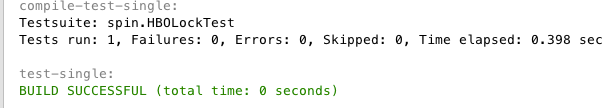
\includegraphics[width=13cm]{HBO01.png}
  \caption{Successful execution of the tests  for Hierarchichal Back-off test}
  \label{fig:HBO01}
\end{figure}
\par
\subsection{Interpretation}
It was shown that the algorithm seems to work and allows synchronization of multiple threads trying to access a shared resource.
\par
One problem however, has to do with the fact that this locking protocol is not fair in the sense that local threads have more chances of acquiring the lock in the next attempt. 
\par
Another thing that we ought to note is that threads spin in the same memory address which causes invalidation of remote cached copies of this value. This problem will be solved yet with another protocol.

% --------------------------- %
% Spin Locks End
% --------------------------- %

% --------------------------- %
% ch 08 Monitors Start
% --------------------------- %
\chapter{Monitors and Blocking Synchronization}
\section{\textbf{QueueTest}}

\subsection{Particular Case (problem)}
The problem we want to solve is again mutual exclusion around a shared
bounded queue; just like chapter 2. The difference here is that, instead of
just using locks the authors try to explain the facilities provided by
Java \C{Condition} interface (part of package
\C{java.util.concurrent.locks}). Such interface, along with the
\C{Lock} one, offer a finer grain control over the
Monitors \footnote{Monitors, as explained in the book, are an
  structured way to integrate synchronization with an object's data
  and methods (speaking about OO paradigm).}
capabilities offered by Java language; when compared to merely using
the \C{synchronized} feature. 

\subsection{Solution}
The solution to the mutual exclusion problem around the bounded queue is
solved by using a single Lock of type \C{ReentrantLock}, to control
exclusive access to the data structure (reentrant is important to
ensure that a thread which has gotten the lock already, can request it
again as many times as it want). In addition, the solution uses a
couple of \C{Condition} objects to represent the conditions 
which enqueuers and dequeuers wait on: \\

\begin{itemize}
  \item \C{notFull}: condition enqueuers wait on, prior daring to push.
  \item \C{notEmpty}: condition dequeuers wait on, prior daring to pop.
\end{itemize}
\hfill

The implementations of methods \C{enq} and \C{deq} are similar to
those from the flawed \C{LockFreeQueue} that we analyzed before; there
are a couple of crucial differences though: \\

\begin{itemize}
\item We use a lock to implement mutual exclusion, so we eliminate all
  the issues seen before due race conditions.
\item The potentially infinite loops for both \C{enq} and \C{deq} now
  do something: they call the \C{await} method on their respective
  conditions. This guarantees that we do not have deadlocks: if a
  thread does not find the queue on the expected state to perform the
  operation, it releases the lock and allow the others to proceed. In
  that way we allow enqueuers to put the data we are waiting for, or
  the dequeuers to make the space we need; after which they
  ``wake-up'' the waiting threads with a call to condition's
  \C{signal} method. 
\end{itemize}
\hfill

The code looks quite similar to our second proposed modification of previous
exercise \C{LockFreeQueueTest}; and actually, it also looks quite
similar to the sample code listed on the \href{http://docs.oracle.com/javase/7/docs/api/java/util/concurrent/locks/Condition.html}{Javadoc API of \C{Condition}
  interface} (on which we also based our proposal). Anyway, the book
solution is listed below for further reference: \\

\begin{lstlisting}[style=numbers]
class Queue<T> {
  final Lock lock = new ReentrantLock();
  final Condition notFull  = lock.newCondition();
  final Condition notEmpty = lock.newCondition();  
  final T[] items; 
  int tail, head, count;  
  public Queue(int capacity) {
    items = (T[])new Object[capacity];
  }
  public void enq(T x) throws InterruptedException {
    lock.lock();
    try {
      while (count == items.length)
        notFull.await();
      items[tail] = x;
      if (++tail == items.length)
        tail = 0;
      ++count;
      notEmpty.signal();
    } finally {
      lock.unlock();
    }
  }  
  public T deq() throws InterruptedException {
    lock.lock();
    try {
      while (count == 0)
        notEmpty.await();
      T x = items[head];
      if (++head == items.length)
        head = 0;
      --count;
      notFull.signal();
      return x;
    } finally {
      lock.unlock();
    }
  }
}
\end{lstlisting}
\hfill

\subsection{Experiment Description}

The test is pretty much the same than \C{LockFreeQueueTest}, except
for the number of threads (8 instead of 2) and data (64 instead of
512). 

\subsection{Observations and Interpretations}
Although the test does not exhibit any issue on 2 nor in 24 cores, we
would feel safer replacing the \C{signal} calls by \C{signalAll}, just
to totally discard the potential problem of lost wake-ups explained on
the book (this is what we did for our second proposal to fix
\C{LockFreeQueueTest}, indeed). A sample successful execution is shown
below: \\ 

\begin{verbatim}
$ junit monitor.QueueTest
.sequential push and pop
.parallel both
.parallel deq
.parallel enq

Time: 0.009

OK (4 tests)
\end{verbatim}
\hfill


% -------------------------------------------------------- %
% Mutex Lock
% by: Isai Barajas Cicourel


% -------------------------------------------------------- %
% Document Start

\section{\textbf{Non-Reentrant Mutual Exclusion}}


% -------------------------------------------------------- %
% Particular Caes

\subsection{Particular Case}
\par
In this experiment we use a re-entrant mutual exclusion Lock with the same basic behavior and semantics as the implicit monitor lock accessed using synchronized methods and statements, but with extended capabilities.
\par


% -------------------------------------------------------- %
% Solution Information

\subsection{Solution}
\par
The Mutex lock extends a \textit{AbstractQueuedSynchronizer}, we have a \textit{tryAcquire()} that only acquire the lock when the state is FREE, an \textit{tryRelease()} that releases the lock by setting the state to FREE and a method to verify the current state of the lock. Due to the AbstractQueued we use a framework for implementing blocking locks and related synchronizers (semaphores, events, etc) that rely on first-in-first-out (FIFO) wait queues. This extended class is designed to be a useful basis for most kinds of synchronizers that rely on a single atomic int value to represent state, thus the object does all the work and we forward the conditions. 
\par
\begin{lstlisting}[frame=single,breaklines=true]
  private final LockSynch sync = new LockSynch();
  
  public void lock() {
    sync.acquire(0);
  }
  public boolean tryLock() {
    return sync.tryAcquire(0);
  }
  public void unlock() {
    sync.release(0);
  }
  public Condition newCondition() {
    return sync.newCondition();
  }
  public boolean isLocked() {
    return sync.isHeldExclusively();
  }
  public boolean hasQueuedThreads() {
    return sync.hasQueuedThreads();
  }
  public void lockInterruptibly() throws InterruptedException {
    sync.acquireInterruptibly(0);
  }
  public boolean tryLock(long timeout, TimeUnit unit) throws InterruptedException {
    return sync.tryAcquireNanos(1, unit.toNanos(timeout));
  }
\end{lstlisting}


% -------------------------------------------------------- %
% Experiment

\subsection{Experiment Description} 
\par
The test creates $8$ threads that need to be coordinate in order to increase a counter. All threads have to cooperate in order to increase the counter into the desire value, this lock implements a explicit lock that the test calls, but with the addition of a re-entrant lock sync, which in addition to implementing the Lock interface, this class defines methods \textit{isLocked()} and \textit{hasQueueThreads()}, as well as some associated protected access methods that may be used for instrumentation and monitoring.
If that is not the case, an assertion fail will be raised.
\par


% -------------------------------------------------------- %
% Results

\subsection{Observations and Interpretations}

\par
The tests executed as expected and no errors where found. Since we extend the AbstractQueuedSynchronizer, we are mainly using the Java java.util.concurrent.locks package.
\begin{lstlisting}[frame=single,breaklines=true]
Tests run: 1, Failures: 0, Errors: 0, Skipped: 0, Time elapsed: 0.382 sec

------------- Standard Output ---------------
parallel
------------- ---------------- ---------------
test-single:
BUILD SUCCESSFUL (total time: 1 second)
\end{lstlisting}





../../zava/Multiprocessor//CountDownLatch.tex
% --------------------------- %
% Monitors End
% --------------------------- %

% --------------------------- %
% ch 09 Linked Lists Start
% --------------------------- %
\chapter{Linked Lists: The Role of Locking}
\section{\textbf{Coarse List}}
% ---------------------------------------------------------------------------- %
\subsection{Particular Case}
\par
In this experiment we are dealing with the problem of creating an algorithm to
create a Snapshot of a set of Register in such a way that the algorithm
garantees a Wait-Free operation.
\par
% ---------------------------------------------------------------------------- %
\subsection{Solution}
\par
The purpose of a Wait-Free snapshot is to overcome the problems of the Simple snapshot presented before. Let us remember that such snapshot executes sucesive collect() operations. Once it achieves a \textit{clean double collect}, it returns the snapshot. Otherwise, it keeps trying. 
\par
One of the ideas behind the Wait-Free Snapshot is that when a double collect fails, it is because a update interfered. That means that the updater could take a snapshot right before its update and other threads could use it as their snapshot too. 
\par
% ---------------------------------------------------------------------------- %
\subsection{Experiment Description}
\par

\par
These are the details of the system we used to run the experiments:
\begin{itemize}
\item Processor: Intel Core i5 @2.5 GHz. 2 Cores.
\item L2 Cache per Core: 256 KB
\item L3 Cache: 3 MB
\item System Memory: 16 GB
\end{itemize}
% ---------------------------------------------------------------------------- %
\subsection{Sample Results}
\par
For this test, we saw that in every try, both test cases passed.
\par
\begin{figure}[h]
  \centering
  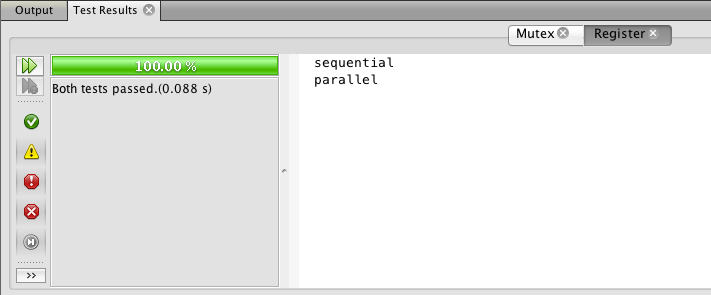
\includegraphics[width=13cm]{WFS00.png}
  \caption{Successful execution of the tests for Wait-Free Snapshot}
  \label{fig:WFS00}
\end{figure}
\par
\begin{figure}[h]
  \centering
  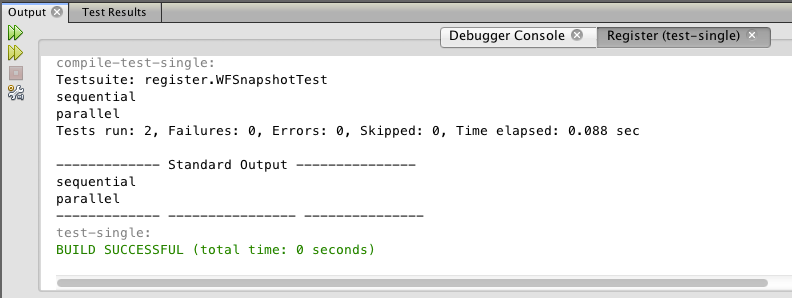
\includegraphics[width=13cm]{WFS01.png}
  \caption{Successful execution of the tests for Wait-Free Snapshot}
  \label{fig:WFS01}
\end{figure}
\par
% ---------------------------------------------------------------------------- %
\subsection{Interpretation}
% ---------------------------------------------------------------------------- %
In this experiment we were able to observe how a Wait-Free Snapshot can be
constructed. 

% -------------------------------------------------------- %
% Fine List
% by: Isai Barajas Cicourel


% -------------------------------------------------------- %
% Document Start

\section{\textbf{Fine-Grained Synchronization List}}


% -------------------------------------------------------- %
% Particular Caes

\subsection{Particular Case}
\par
The Fine-Grained synchronization improves concurrency by locking individual nodes, rather than locking the list as a whole. Instead of placing a lock on the entire list, we add a Lock to each node, along with \textit{lock()} and \textit{unlock()} methods.
\par


% -------------------------------------------------------- %
% Solution Information

\subsection{Solution}
\par
Just as in the coarse-grained list, \textit{remove()} makes currA unreachable by setting predA next field to currA successor. To be safe, \textit{remove()} must lock both predA and currA. To guarantee progress, it is important that all methods acquire locks in the same order, starting at the head and following next references toward the tail.
The \textit{FineList} class \textit{add()} method uses hand-over-hand locking to traverse the list. The finally blocks release locks before returning. 
\par
\begin{lstlisting}[frame=single,breaklines=true]
  public boolean add(T item) {
    int key = item.hashCode();
    head.lock();
    Node pred = head;
    try {
      Node curr = pred.next;
      curr.lock();
      try {
        while (curr.key < key) {
          pred.unlock();
          pred = curr;
          curr = curr.next;
          curr.lock();
        }
        if (curr.key == key) {
          return false;
        }
        Node newNode = new Node(item);
        newNode.next = curr;
        pred.next = newNode;
        return true;
      } finally {
        curr.unlock();
      }
    } finally {
      pred.unlock();
    }
  }
\end{lstlisting}
\begin{lstlisting}[frame=single,breaklines=true]
  public boolean remove(T item) {
    Node pred = null, curr = null;
    int key = item.hashCode();
    head.lock();
    try {
      pred = head;
      curr = pred.next;
      curr.lock();
      try {
        while (curr.key < key) {
          pred.unlock();
          pred = curr;
          curr = curr.next;
          curr.lock();
        }
        if (curr.key == key) {
          pred.next = curr.next;
          return true;
        }
        return false;
      } finally {
        curr.unlock();
      }
    } finally {
      pred.unlock();
    }
  }
\end{lstlisting}

% -------------------------------------------------------- %
% Experiment

\subsection{Experiment Description} 
\par
The test creates $8$ threads that need to be coordinate in order to add and remove values from a list. All threads have to cooperate in order to parallel add and remove values from the list while avoiding duplicate remove of the values.
If that is not the case, a fail will be raised.
\par


% -------------------------------------------------------- %
% Results

\subsection{Observations and Interpretations}

\par
The tests executed as expected and no errors where found. 
\begin{lstlisting}[frame=single,breaklines=true]
Tests run: 4, Failures: 0, Errors: 0, Skipped: 0, Time elapsed: 0,183 sec

------------- Standard Output ---------------
sequential add, contains, and remove
parallel add
parallel remove
parallel both
------------- ---------------- ---------------
test-single:
BUILD SUCCESSFUL (total time: 2 seconds)
\end{lstlisting}





% -------------------------------------------------------- %
% Optimistic List
% by: Isai Barajas Cicourel


% -------------------------------------------------------- %
% Document Start

\section{\textbf{Optimistic Synchronization}}


% -------------------------------------------------------- %
% Particular Caes

\subsection{Particular Case}
\par
In this experiment, the particular case we are trying to study an Optimistic Synchronization which to reduce synchronization costs we take a chance by, search without acquiring locks, lock the nodes found, and then confirm that the locked nodes are correct.
\par


% -------------------------------------------------------- %
% Solution Information

\subsection{Solution}
\par
The \textit{OptimisticList} \textit{add()} method traverses the list ignoring locks, acquires locks, and validates before adding the new node, we must validate and guarantee freedom from interference by checking that predA points to currA and is reachable from head.
\par
\begin{lstlisting}[frame=single,breaklines=true]
  public boolean add(T item) {
    int key = item.hashCode();
    while (true) {
      Entry pred = this.head;
      Entry curr = pred.next;
      while (curr.key <= key) {
        pred = curr; curr = curr.next;
      }
      pred.lock(); curr.lock();
      try {
        if (validate(pred, curr)) {
          if (curr.key == key) { // present
            return false;
          } else {               // not present
            Entry entry = new Entry(item);
            entry.next = curr;
            pred.next = entry;
            return true;
          }
        }
      } finally {                // always unlock
        pred.unlock(); curr.unlock();
      }
    }
  }
\end{lstlisting}
The \textit{remove()} method traverses ignoring locks, acquires locks, and validates before removing the node.
\par
\begin{lstlisting}[frame=single,breaklines=true]
  public boolean remove(T item) {
    int key = item.hashCode();
    while (true) {
      Entry pred = this.head;
      Entry curr = pred.next;
      while (curr.key < key) {
        pred = curr; curr = curr.next;
      }
      pred.lock(); curr.lock();
      try {
          if (validate(pred, curr)) {
            if (curr.key == key) { // present in list
              pred.next = curr.next;
              return true;
            } else {               // not present in list
              return false;
            }
          }
      } finally {                // always unlock
        pred.unlock(); curr.unlock();
      }
    }
  }
\end{lstlisting}


% -------------------------------------------------------- %
% Experiment

\subsection{Experiment Description} 
\par
The test creates $8$ threads that need to be coordinate in order to add and remove values from a list. All threads have to cooperate in order to parallel add and remove values from the list while avoiding duplicate remove of the values.
If that is not the case, a fail will be raised.
\par

% -------------------------------------------------------- %
% Results

\subsection{Observations and Interpretations}

\par
When executing the test duplicate removes where found.
\begin{lstlisting}[frame=single,breaklines=true]
junit.framework.AssertionFailedError: RemoveThread: duplicate remove: 
\end{lstlisting}


% -------------------------------------------------------- %
% Results

\subsection{Proposed changes to fix the problem}

\par
The test approach is naive, since it assumes that data would exist always prior deletion, thus not handling the case when there is no data to remove.
By doing a retry until there is data to remove the problem seems to be fix.
\begin{lstlisting}[frame=single,breaklines=true]
  public boolean remove(T item) {
    int key = item.hashCode();
    boolean bRetry = true;
    while (true) {
      Entry pred = this.head;
      Entry curr = pred.next;
      while (curr.key < key) {
        pred = curr; curr = curr.next;
      }
      pred.lock(); curr.lock();
      try {
        while (bRetry) {
          if (validate(pred, curr)) {
            bRetry = false;
            if (curr.key == key) { // present in list
              pred.next = curr.next;
              return true;
            } else {               // not present in list
              return false;
            }
          }
        }
      } finally {                // always unlock
        pred.unlock(); curr.unlock();
      }
    }
  }
}
\end{lstlisting}
Once the change is made the execution works fine on every equipment used.
\begin{lstlisting}[frame=single,breaklines=true]
Tests run: 4, Failures: 0, Errors: 0, Skipped: 0, Time elapsed: 0,071 sec

------------- Standard Output ---------------
sequential add, contains, and remove
parallel add
parallel remove
parallel both
------------- ---------------- ---------------
test-single:
BUILD SUCCESSFUL (total time: 3 seconds)
\end{lstlisting}


% -------------------------------------------------------- %
% Why?

\subsection{Proposed solution}
\par
This error may imply a bad scheduling of the list. Apparently old JVM depending on the OS, executed using a logic that avoided this from happening by working in a round robin fashion.


\section{\textbf{LazyListTest}}

\subsection{Particular Case (problem)}
The problem is that of gradually improving what coarse grain locking
offers for concurrent data structures like sets (implemented with
linked lists).

\subsection{Solution}
The \C{LazyList} solution is a refinement of the \C{OptimisticList}
solution which does not lock while searching, but locks one it finds
the interesting nodes (and then confirms that the locked nodes are
correct). As one drawback of \C{OptimisticList} is that the most
common method \C{contains} method locks, the next logical improvement
is to make this method wait-free while keeping the \C{add} and
\C{remove} methods locking (but reducing their transversings of the
list from two to just one). \\

The refinement mentioned above is precisely that of \C{LazyList},
which adds a new bit to each node to indicate whether they still
belong to the set or not (this prevents transvering the list to detect
if the node is reachable, as the new bit introduces such invariant: if
a transversing thread does not find a node or it is marked in this
bit, then the corresponding item does not belong to the set. This
behavior implies that \C{contains} method does a single wait-free
transversal of the list. \\

For adding an element to the list, \C{add} method traverses the list,
locks the target's predecessor and successor nodes, and inserts the
new node in between. The \C{remove}   
method is lazy (hence the name of the solution), as it splits its task in
two parts: first marks the node in the new bit, logically removing it;
and second, update its predecessor's next field, physically removing
it. \\

The three methods ignore the locks while transversing the list,
possibly passing over both logically and physically deleted nodes. The
\C{add} and \C{remove} methods still lock \C{pred} and \C{curr} nodes
as with \C{OptimisticList} solution, but the validation reduces to
check that \C{curr} node has not been marked; as well as validating
the same for \C{pred} node, and that it still points to \C{curr}
(validating a couple of nodes is much better than transversing whole
list though). Finally, the introduction of logical removals implies a
new contract for detecting that an item still belongs to set: it does
so, if still referred by an unmarked reachable node. \\

The most relevant methods, \C{remove} and \C{contains}, are listed
below: \\

\begin{lstlisting}[style=numbers]
  public boolean remove(T item) {
    int key = item.hashCode();
    while (true) {
      Node pred = this.head;
      Node curr = head.next;
      while (curr.key < key) {
        pred = curr; curr = curr.next;
      }
      pred.lock();
      try {
        curr.lock();
        try {
          if (validate(pred, curr)) {
            if (curr.key != key) {    // present
              return false;
            } else {                  // absent
              curr.marked = true;     // logically remove
              pred.next = curr.next;  // physically remove
              return true;
            }
          }
        } finally {                   // always unlock curr
          curr.unlock();
        }
      } finally {                     // always unlock pred
        pred.unlock();
      }
    }
  }

  public boolean contains(T item) {
    int key = item.hashCode();
    Node curr = this.head;
    while (curr.key < key)
      curr = curr.next;
    return curr.key == key && !curr.marked;
  }
\end{lstlisting}
\hfill

\subsection{Experiment Description}
The test is pretty much the same described for \C{LockFreeQueueTest},
with a few differences.

\begin{itemize}
\item The data structure here is a set, rather than a queue.
\item The exception that it uses 8 threads instead of two for each
  operation (\C{add} / \C{remove}).
\item The threads that remove elements do not care only in
  successfully removing certain number of times (like with the queue);
  here they expect to remove a particular subset of the values.
\end{itemize}
  

\subsection{Observations and Interpretations}

The test works as expected on a two cores machine, sample output below:

\begin{verbatim}
.parallel deq
.parallel both
.sequential push and pop
.parallel enq

Time: 0.03

OK (4 tests)
\end{verbatim}
\hfill

Interestingly, on a 24 cores machine, sometimes the test case
\C{testParallelBoth} fails with exceptions like the one below: \\

\begin{verbatim}
junit.framework.AssertionFailedError: RemoveThread: duplicate remove
at junit.framework.Assert.fail(Assert.java:57)
at junit.framework.TestCase.fail(TestCase.java:227)
at lists.LazyListTest$RemoveThread.run(LazyListTest.java:142)
\end{verbatim}
\hfill

While debugging the error above, we found that the message of
``duplicate remove'' is a bit misleading; is not really that someone
else tried to delete that value (as each \C{RemoveThread} cares about
a unique set of values). The real problem is that the removing threads
just try once to remove each value, and fail if they did not find any
of them. Since both the adder and remover threads are started
concurrently, there is no guarantee that the adders will come first
than the removers; so it could be that the removers try to pull out
something that has not been inserted yet (leaving to the exception
shown above). \\

Since the \C{LazyList} solution does not include an error-and-retry
approach (as with our second rewrite of the \C{LockFreeQueue}, which
used Java condition's await methods), the only way to fix this would
be to rewrite the test program itself. Each remover thread will need
to indefinitely try to remove all its items until completion, rather
than expecting that all of them are available by the time they are to
be removed. We tried that approach and made the proper adjustments
to the test program, after which the problem got solved as expected.

\section{\textbf{Lock-Free List}}
% ---------------------------------------------------------------------------- %
\subsection{Particular Case}
\par
We have seen some algorithms for implementing a concurrent list. Now it is time
to see how a Lock-Free implementation can be done.
\par
% ---------------------------------------------------------------------------- %
\subsection{Solution}
\par
\par
% ---------------------------------------------------------------------------- %
\subsection{Experiment Description}
\par
Again, we have the same four test cases that we have been dealing with:
\par
\begin{enumerate}
\item \textit{testSequential()}. The main thread inserts multiple elements to
the list, then checks if all elements are there and finally removes all elements
one by one.
\item \textit{testParallelAdd()}. The main thread spawns multiple threads that
add elements to the list concurrently. When they are done, the main thread
checks if all elements are in there and finally removes all elements.
\item \textit{testParallelRemove()}. The main thread inserts multiple elements
to the list, then checks if all elements are in there and finally it spawns
multiple threads that remove the elements from the list concurrently.
\item \textit{testParallelBoth()}. The main thread creates multiple threads.
Some of them insert elements to the list and some of them remove elements.
\end{enumerate}
\par
% ---------------------------------------------------------------------------- %
\subsection{Sample Results}
\par
Similar to the other implementations, the test cases turns out to have a
problem. Here is the output:
\par
\begin{verbatim}
[oraadm@gdlaa008 Lists]$ junit lists.LockFreeListTest
.sequential add, contains, and remove
.parallel both
Exception in thread "Thread-13" junit.framework.AssertionFailedError:
RemoveThread: duplicate remove: 109
        at junit.framework.Assert.fail(Assert.java:57)
        at junit.framework.TestCase.fail(TestCase.java:227)
        at lists.LockFreeListTest$RemoveThread.run(LockFreeListTest.java:145)
.parallel add
.parallel remove

Time: 0.022

OK (4 tests)
\end{verbatim}
\par
The fix for this is the same that has been discussed before. Here is the test
output after the fix:
\begin{verbatim}
[oraadm@gdlaa008 Lists]$ junit lists.LockFreeListTest
.sequential add, contains, and remove
.parallel both
.parallel add
.parallel remove

Time: 0.016

OK (4 tests)
\end{verbatim}
\par
% ---------------------------------------------------------------------------- %
\subsection{Interpretation}
% ---------------------------------------------------------------------------- %
We observed a way in which a list could be implemented allowing it to be lock
free. When using the same set of unit tests as before, we see that the
implementation works correctly.

% --------------------------- %
% Linked Lists End
% --------------------------- %

% --------------------------- %
% ch 10 Concurrent Queues Start
% --------------------------- %
\chapter{Concurrent Queues and the ABA Problem}
% --------------------------- %
% LockFreeQueueTest Start
% --------------------------- %
\section{\textbf{LockFreeQueueTest Test}}
%%%%%%%%%%%%%%%%%%%%%%%%%%%%%%%%%%
\subsection{Particular Case}
\par
In this exercise we deal with the problem of implementing a Queue data
structure with the particular characteristic of being lock free. 
\par
%%%%%%%%%%%%%%%%%%%%%%%%%%%%%%%%%%
\subsection{Solution}
\par
Here we present the implementation of the Lock Free Queue that is based on the paper by Michael and Scott. 
\par
Here is the \textit{enqueue()} method:
\par
\hfill
\begin{lstlisting}[style=numbers]
  /**
   * Append item to end of queue.
   * @param item
   */
  public void enq(T item) {
    if (item == null) throw new NullPointerException();
    Node node = new Node(item); // allocate & initialize new node
    while (true) {		 // keep trying
      Node last = tail.get();    // read tail
      Node next = last.next.get(); // read next
      if (last == tail.get()) { // are they consistent?
        AtomicReference[] target = {last.next, tail};
        Object[] expect = {next, last};
        Object[] update = {node, node};
        if (multiCompareAndSet(
            (AtomicReference<T>[]) target,
            (T[]) expect,
            (T[]) update)){
          return;
        }
      }
    }
  }
\end{lstlisting}
\hfill
\par
Here is the dequeue method.
\par
\hfill
\begin{lstlisting}[style=numbers]
  /**
   * Remove and return head of queue.
   * @return remove first item in queue
   * @throws queue.EmptyException
   */
  public T deq() throws EmptyException {
    while (true) {
      Node first = head.get();
      Node last = tail.get();
      Node next = first.next.get();
      if (first == head.get()) {// are they consistent?
        if (first == last) {	// is queue empty or tail falling behind?
          if (next == null) {	// is queue empty?
            throw new EmptyException();
          }
          // tail is behind, try to advance
          tail.compareAndSet(last, next);
        } else {
          T value = next.value; // read value before dequeuing
          if (head.compareAndSet(first, next))
            return value;
        }
      }
    }
\end{lstlisting}
\hfill
\par
%%%%%%%%%%%%%%%%%%%%%%%%%%%%%%%%%%
\subsection{Experiment Description}
\par
The test consists of 4 test cases. Let us briefly describe each one of them:
\par
\begin{itemize}
\item testSequential. In this test case 512 elements are enqueued in the data
structure. After that, each of the elements are dequeued. At each dequeue, we
verify that the dequeued elements are in sequential order (just as they were
inserted).
\item testParallelEnqueue. This test cases spawns $8$ enqueuer threads. Each of
them will add 512 elements to the queue. When they are done, the main thread
dequeues each of the elements performing the same check described above.
\item testParallelDequeue. In this test case, the master thread enqueues 512
elements. When done, 8 dequeuer threads are spawned. The job of each of these
dequeuer threads is to remove the elements. Additionally, an array that keeps
track of which elements have been already dequeued is maintained. The test
checks that no element is removed more than once.
\item testParallelBoth. This is the most complete test in the suite. It spawns
8 enqueuer threads and 8 dequeuer threads. Each enqueuer adds 512 elements to
the queue. The dequeuers must remove each of these elements. A check similar to
the one described in the \textit{testParallelDequeue} test is performed.
\end{itemize}
\par
%%%%%%%%%%%%%%%%%%%%%%%%%%%%%%%%%%
\subsection{Sample Results and Interpretation}
\par
As it is, the test fails as follows:
\par
\hfill
\begin{verbatim}
[oraadm@gdlaa008 Queue]$ junit queue.LockFreeQueueTest
.sequential push and pop
F.parallel both
.parallel deq
.parallel enq
E
Time: 0.012
There was 1 error:
1) testParallelEnq(queue.LockFreeQueueTest)queue.EmptyException
  at queue.LockFreeQueue.deq(LockFreeQueue.java:64)
  at queue.LockFreeQueueTest.testParallelEnq(LockFreeQueueTest.java:69)
  at sun.reflect.NativeMethodAccessorImpl.invoke0(Native Method)
  at
sun.reflect.NativeMethodAccessorImpl.invoke(NativeMethodAccessorImpl.java:57)
  at
sun.reflect.DelegatingMethodAccessorImpl.invoke(DelegatingMethodAccessorImpl.java:43)
There was 1 failure:
1) testSequential(queue.LockFreeQueueTest)junit.framework.AssertionFailedError:
unexpected empty queue
  at queue.LockFreeQueueTest.testSequential(LockFreeQueueTest.java:51)
  at sun.reflect.NativeMethodAccessorImpl.invoke0(Native Method)
  at
sun.reflect.NativeMethodAccessorImpl.invoke(NativeMethodAccessorImpl.java:57)
  at
sun.reflect.DelegatingMethodAccessorImpl.invoke(DelegatingMethodAccessorImpl.java:43)

FAILURES!!!
Tests run: 4,  Failures: 1,  Errors: 1
\end{verbatim}
\hfill
\par
The problem with it, is that it is using a stub function for
multi-compareAndSet:
\par
\hfill
\begin{lstlisting}[style=numbers]
  private static <T> boolean multiCompareAndSet(
      AtomicReference<T>[] target,
      T[] expect,                                                                                                                                                                    
      T[] update) {
    return true;
  }
\end{lstlisting}
\hfill
\par
Actually, what we did to get around it, is to implement the enqueue code as the
book says, that is:
\hfill
\begin{lstlisting}[style=numbers]
  /**                                                                                                                                                                                
   * Append item to end of queue.
   * @param item
   */
  public void enq(T item) {
    if (item == null) throw new NullPointerException();
    Node node = new Node(item); // allocate & initialize new node
    while (true) {     // keep trying
      Node last = tail.get();    // read tail
      Node next = last.next.get(); // read next
      if (last == tail.get()) { // are they consistent?
        if (next == null) {
          if (last.next.compareAndSet(next,node)) {
            tail.compareAndSet(last,node);
            return;
          }   
        }   
        else {
          tail.compareAndSet(last,next);
        }   
      }   
    }
  }   
\end{lstlisting}
\hfill
\par
After that, we were able to successfully execute the test cases:
\par
\hfill
\begin{verbatim}
[oraadm@gdlaa008 Queue]$ junit queue.LockFreeQueueTest
.sequential push and pop
.parallel both
.parallel deq
.parallel enq

Time: 0.016

OK (4 tests)
\end{verbatim}
\hfill
\par
%%%%%%%%%%%%%%%%%%%%%%%%%%%%%%%%%%
% --------------------------- %
% LockFreeQueueTest End
% --------------------------- %

% -------------------------------------------------------- %
% HW Queue
% by: Isai Barajas Cicourel


% -------------------------------------------------------- %
% Document Start

\section{\textbf{HW Queue}}


% -------------------------------------------------------- %
% Particular Caes

\subsection{Particular Case}
\par
The HW Queue uses the Atomic values defined by the Java language in order to implement a locking free queue.
\par


% -------------------------------------------------------- %
% Solution Information

\subsection{Solution}
\par
The unbounded queue implementation used by the \textit{HWQueue} class is blocking, meaning that the \textit{deq()} method does not return until it has found an item to dequeue.  
\par
\begin{lstlisting}[frame=single,breaklines=true]
  public T deq() {
    while (true) {
      int range = tail.get();
      for (int i = 0; i < range; i++) {
        T value = items[i].getAndSet(null);
        if (value != null) {
          return value;
        }
      }
    }
  }
\end{lstlisting}
\par
The \textit{enq()} method uses the \textit{AtomicInteger} \textit{getAndIncrement()} method that atomically incremented the counter.
\par
\begin{lstlisting}[frame=single,breaklines=true]
  public void enq(T x) {
    int i = tail.getAndIncrement();
    items[i].set(x);
  }
\end{lstlisting}

% -------------------------------------------------------- %
% Experiment

\subsection{Experiment Description} 
\par
The test creates $8$ threads that need to be coordinate in order to add and remove values from a list. All threads have to cooperate in order to parallel add and remove values from the list while avoiding duplicate remove of the values.
If that is not the case, a fail will be raised.
\par


% -------------------------------------------------------- %
% Results

\subsection{Observations and Interpretations}

\par
The tests executed as expected and no errors where found. 
\begin{lstlisting}[frame=single,breaklines=true]
Tests run: 4, Failures: 0, Errors: 0, Skipped: 0, Time elapsed: 0,121 sec

------------- Standard Output ---------------
sequential push and pop
parallel enq
parallel deq
parallel both
------------- ---------------- ---------------
test-single:
BUILD SUCCESSFUL (total time: 1 second)
\end{lstlisting}





\newpage
\section{\textbf{BoundedQueueTest}}

\subsection{Particular Case (problem)}
The problem is to implement a bounded partial queue (that is, one
which finite capacity which allows waits inside its methods). 

\subsection{Solution}
The solution proposes to allow concurrency among enqueuers and
dequeuers, by using two different locks (one for each group of
threads). The code is small enough to be placed and explained in a bit
more detail here, so let us give it a try:

\begin{lstlisting}[style=numbers]
  public void enq(T x) {
    if (x == null) throw new NullPointerException();
    boolean mustWakeDequeuers = false;
    enqLock.lock();
    try {
      while (size.get() == capacity) {
        try {
          notFullCondition.await();
        } catch (InterruptedException e) {}
      }
      Entry e = new Entry(x);
      tail.next = e;
      tail = e;
      if (size.getAndIncrement() == 0) {
        mustWakeDequeuers = true;
      }
    } finally {
      enqLock.unlock();
    }
    if (mustWakeDequeuers) {
      deqLock.lock();
      try {
        notEmptyCondition.signalAll();
      } finally {
        deqLock.unlock();
      }
    }
  }
\end{lstlisting}
\hfill

The main points of algorithm above are as follows (the code above was
previously corrected, as it had several things inverted):

\begin{itemize}
\item It does not allow null values.
\item There is a lock dedicated to \C{enq} method, which guarantees
  mutual exclusion to the critical section for enqueuers.
\item It spins while the queue is full (the try/catch block was added
  just to allow compilation). This line was incorrectly asking whether
  queue was empty, while it needs to ask whether is still full.
\item  Once we know queue is room, we allocate the new node and update
  \C{tail} pointer.
\item We atomically get and increment the atomic counter for the size
  (this was previously a decrement, which was incorrect).
\item If the atomically retrieved previous value of size was zero, it
  means the queue was empty and there may had been waiting dequeuers;
  therefore we acquire the lock for \C{deq} method and inform all
  dequeuers that the queue has not at least an item.
\end{itemize}
\hfill

The \C{deq} method is symmetric so we do not repeat same explanation
(but worth to say that it had same inverted conditions and actions
than \C{enq} method, in the code; so we needed to apply same
corrective actions ... perhaps that was the purpose of the exercise?).

\subsection{Experiment Description}
The test is pretty much the same described for \C{LockFreeQueueTest}.
(with the exceptiont that it uses 8 threads instead of two).

\subsection{Observations and Interpretations}
The original code for the test made no sense, as conditions and
actions for \C{enq} and \C{deq} methods were inverted; we did not even
care testing such strange version that did not match at all the one
published on the book (we also needed to fix the initialization of the
\C{size} variable, which shall be zero instead of \C{capacity}). After
the corrections mentioned on the Solution section above, the test ran
normally. Sample output below: 

\begin{verbatim}
.parallel both
.sequential push and pop
.parallel enq
.parallel deq

Time: 0.028

OK (4 tests)
\end{verbatim}
\hfill

Even if the original version of this test actually ran (we did not
test it), it turns out quite counter-intuitive. The modified code worked fine
on both 2 and 24 core machines.



% -------------------------------------------------------- %
% Unbounded Queue
% by: Isai Barajas Cicourel


% -------------------------------------------------------- %
% Document Start

\section{\textbf{Unbounded Queue}}


% -------------------------------------------------------- %
% Particular Caes

\subsection{Particular Case}
\par
In this experiment we implement a unbounded queue, the representation is the same as the bounded queue, except there is no need to count the number of items in the queue, or to provide conditions on which to wait.
\par


% -------------------------------------------------------- %
% Solution Information

\subsection{Solution}
\par
According to the theory an item is actually enqueued when the \textit{enq()} call sets the last node’s next field to the new node, even before \textit{enq()} resets tail to refer to the new node. After that instant, the new item is reachable along a chain of the next references. 
The actual head is the successor of the node referenced by head, and the actual tail is the last item reachable from the head. Both the \textit{enq()} and \textit{deq()} methods are total as they do not wait for the queue to become empty or full.
\par
\begin{lstlisting}[frame=single,breaklines=true]
  public T deq() throws EmptyException {
    T result;
    deqLock.lock();
    try {
      if (head.next == null) {
        throw new EmptyException();
      }
      result = head.next.value;
      head = head.next;
    } finally {
      deqLock.unlock();
    }
    return result;
  }
\end{lstlisting}
\par
\begin{lstlisting}[frame=single,breaklines=true]
  public void enq(T x) {
    if (x == null) throw new NullPointerException();
    enqLock.lock();
    try {
      Node e = new Node(x);
      tail.next = e;
      tail = e;
    } finally {
      enqLock.unlock();
    }
  }
\end{lstlisting}
\par
This queue cannot deadlock, because each method acquires only one lock, either \textit{enqLock} or \textit{deqLock} and is much simpler than the bounded queue.

% -------------------------------------------------------- %
% Experiment

\subsection{Experiment Description} 
\par
The test creates $8$ threads that need to be coordinate in order to \textit{enq()} and \textit{deq()} a range of numbers. All threads have to cooperate to add and remove elements from the queue. Each of the threads will enqueue and dequeue values into the queue, if everything works according to the test there will be mutual exclusion and the mapping of elements will corresponds to the queue elements.
If that is not the case, a duplicate fail will be raised.
\par


% -------------------------------------------------------- %
% Results

\subsection{Observations and Interpretations}

\par
The tests executed as expected and no errors where found. Since the \textit{ReentrantLock} is used to acquire an explicit lock, the mutual exclusion is guarantee by the Java java.util.concurrent.locks package.
As a interesting note, once each $100$ executions the running time increases exponentially as shown below.
\begin{lstlisting}[frame=single,breaklines=true]
Tests run: 4, Failures: 0, Errors: 0, Skipped: 0, Time elapsed: 10,102 sec

------------- Standard Output ---------------
sequential push and pop
parallel enq
parallel deq
parallel both
------------- ---------------- ---------------
test-single:
BUILD SUCCESSFUL (total time: 11 seconds)
\end{lstlisting}





../../dario/Multiprocessor//SynchronousDualQueueTest.tex
% --------------------------- %
% SynchronousQueueTest Start
% --------------------------- %
\section{\textbf{SynchronousQueueTest}}
%%%%%%%%%%%%%%%%%%%%%%%%%%%%%%%%%%
\subsection{Particular Case}
\par
In this exercise we are dealing again with a first-in-first-out (FIFO) data
structure, i.e. a Queue. The difference with respect of the previous examples is
that in this case we have multiple producers and multiple consumers
\textit{rendezvous}ing with one another. In other words, a producer that puts
an item in the queue blocks until that item is removed by a consumer.
\par
%%%%%%%%%%%%%%%%%%%%%%%%%%%%%%%%%%
\subsection{Solution}
\par
The following is a naive implementation of a Synchronous queue. Notice that it
contains the following fields:
\par
\hfill
\begin{lstlisting}[style=numbers]
  public class SynchronousQueue<T> {
    T item = null;
    boolean enqueuing;
    Lock lock;
    Condition condition;
	...
	}
\end{lstlisting}
\hfill
\par
Let us talk about them:
\begin{itemize}
\item item. The first item in the queue (the one to be dequeued)
\item enqueuing. Used to sync the enqueuers
\item lock. Used for mutual exclusion
\item condition. Used to block partial methods
\end{itemize}
\par
Now, let us talk about how the enqueue and the dequeue actually work:
\par
\hfill
\begin{lstlisting}[style=numbers]
    public T deq() throws InterruptedException {
      lock.lock();
      try {
        while (item == null) {
          condition.await();
        }
        T t = item;
        item = null;
        condition.signalAll();
        return t;
      } finally {
        lock.unlock();
      }
    }

    public void enq(T value) throws InterruptedException {
      if (value == null) throw new NullPointerException();
      try {
        while (enqueuing) { // another enqueuer's turn
          condition.await();
        }
        enqueuing = true; // my turn starts
        item = value;
        condition.signalAll();
        while (item != null) {
          condition.await();
        }
        enqueuing = false;  // my turn ends
        condition.signalAll();
      } finally {
        lock.unlock();
      }
    }
  }
\end{lstlisting}
\hfill
\par
The enqueue method first has to check whether another enqueuer is enqueueng an
element. If that is the case, then the enqueuer has to wait till the enqueuer
is paired with a dequeuer. After that, it will set the flag \textit{enqueuing}
to true, sets the item and signals any other thread that is waiting for this
one to finish its enqueue. 
\par
Once the enqueuer has put its value in the queue, it waits till someone
consumes its value (\textit{item} becomes \textit{null}). Then the enqueuer
sets the \textit{enqueuing} flag back to false and finishes.
\par
On the other hand, the dequeuer threads after acquiring the lock, they have to
wait till an element is put in the queue. When it finds this is true, then they
take the item and signal other threads to indicate they have finished
dequeuing.
\par
%%%%%%%%%%%%%%%%%%%%%%%%%%%%%%%%%%
\subsection{Experiment Description}
\par
This exercise consists of only one test and it works as follow:
\par
It creates $2*8$ threads. Each of the threads will enqueue $512/8$ elements to
the queue. At the same time, $8$ threads will try to dequeue the elements. When
dequeueing, the test will put a value of \textit{true} in the slot
$arr[value]$. The test expects that each slot should not be set to
\textit{true} twice.
\par
%%%%%%%%%%%%%%%%%%%%%%%%%%%%%%%%%%
\subsection{Sample Results}
\par
First, we need to mention that we had a problem compiling the test cases because
we needed to add a try-catch block around the \textit{enq()} \textit{deq()}
call like this:
\par
\hfill
\begin{lstlisting}[style=numbers]
        try{
          int value = (Integer)instance.deq();
          if (map[value]) {
            fail("DeqThread: duplicate pop");
          }
          map[value] = true;                                                                                                                                                         
        } catch(InterruptedException ie) {
          System.out.println("Exception" + ie);
        }
\end{lstlisting}
\hfill
\par
After that, we noticed that they consistently fails with the following error:
\par
\hfill
\begin{verbatim}
[oraadm@gdlaa008 Queue]$ junit queue.SynchronousQueueTest
.parallel both
Exception in thread "Thread-10" Exception in thread "Thread-6" Exception in thread "Thread-2" Exception in th
read "Thread-0" Exception in thread "Thread-8" Exception in thread "Thread-4" Exception in thread "Thread-14"
 Exception in thread "Thread-12" java.lang.IllegalMonitorStateException
        at java.util.concurrent.locks.ReentrantLock$Sync.tryRelease(ReentrantLock.java:155)
        at java.util.concurrent.locks.AbstractQueuedSynchronizer.release(AbstractQueuedSynchronizer.java:1260)
        at java.util.concurrent.locks.ReentrantLock.unlock(ReentrantLock.java:460)
        at queue.SynchronousQueue.enq(SynchronousQueue.java:63)
        at queue.SynchronousQueueTest$EnqThread.run(SynchronousQueueTest.java:61)
java.lang.IllegalMonitorStateException
        at java.util.concurrent.locks.ReentrantLock$Sync.tryRelease(ReentrantLock.java:155)
        at java.util.concurrent.locks.AbstractQueuedSynchronizer.release(AbstractQueuedSynchronizer.java:1260)
        at java.util.concurrent.locks.ReentrantLock.unlock(ReentrantLock.java:460)
        at queue.SynchronousQueue.enq(SynchronousQueue.java:63)
        at queue.SynchronousQueueTest$EnqThread.run(SynchronousQueueTest.java:61)
java.lang.IllegalMonitorStateException
        at java.util.concurrent.locks.ReentrantLock$Sync.tryRelease(ReentrantLock.java:155)
        at java.util.concurrent.locks.AbstractQueuedSynchronizer.release(AbstractQueuedSynchronizer.java:1260)
        at java.util.concurrent.locks.ReentrantLock.unlock(ReentrantLock.java:460)
        at queue.SynchronousQueue.enq(SynchronousQueue.java:63)
        at queue.SynchronousQueueTest$EnqThread.run(SynchronousQueueTest.java:61)
java.lang.IllegalMonitorStateException
        at java.util.concurrent.locks.ReentrantLock$Sync.tryRelease(ReentrantLock.java:155)
        at java.util.concurrent.locks.AbstractQueuedSynchronizer.release(AbstractQueuedSynchronizer.java:1260)
        at java.util.concurrent.locks.ReentrantLock.unlock(ReentrantLock.java:460)
        at queue.SynchronousQueue.enq(SynchronousQueue.java:63)
        at queue.SynchronousQueueTest$EnqThread.run(SynchronousQueueTest.java:61)
java.lang.IllegalMonitorStateException
        at java.util.concurrent.locks.ReentrantLock$Sync.tryRelease(ReentrantLock.java:155)
        at java.util.concurrent.locks.AbstractQueuedSynchronizer.release(AbstractQueuedSynchronizer.java:1260)
        at java.util.concurrent.locks.ReentrantLock.unlock(ReentrantLock.java:460)
        at queue.SynchronousQueue.enq(SynchronousQueue.java:63)
        at queue.SynchronousQueueTest$EnqThread.run(SynchronousQueueTest.java:61)
java.lang.IllegalMonitorStateException
        at java.util.concurrent.locks.ReentrantLock$Sync.tryRelease(ReentrantLock.java:155)
        at java.util.concurrent.locks.AbstractQueuedSynchronizer.release(AbstractQueuedSynchronizer.java:1260)
        at java.util.concurrent.locks.ReentrantLock.unlock(ReentrantLock.java:460)
        at queue.SynchronousQueue.enq(SynchronousQueue.java:63)
        at queue.SynchronousQueueTest$EnqThread.run(SynchronousQueueTest.java:61)
java.lang.IllegalMonitorStateException
        at java.util.concurrent.locks.ReentrantLock$Sync.tryRelease(ReentrantLock.java:155)
        at java.util.concurrent.locks.AbstractQueuedSynchronizer.release(AbstractQueuedSynchronizer.java:1260)
        at java.util.concurrent.locks.ReentrantLock.unlock(ReentrantLock.java:460)
        at queue.SynchronousQueue.enq(SynchronousQueue.java:63)
        at queue.SynchronousQueueTest$EnqThread.run(SynchronousQueueTest.java:61)
java.lang.IllegalMonitorStateException
        at java.util.concurrent.locks.ReentrantLock$Sync.tryRelease(ReentrantLock.java:155)
        at java.util.concurrent.locks.AbstractQueuedSynchronizer.release(AbstractQueuedSynchronizer.java:1260)
        at java.util.concurrent.locks.ReentrantLock.unlock(ReentrantLock.java:460)
        at queue.SynchronousQueue.enq(SynchronousQueue.java:63)
        at queue.SynchronousQueueTest$EnqThread.run(SynchronousQueueTest.java:61)
\end{verbatim}
\par
The problem is a bad use of the monitor API. Here is the corrected code:
\par
\hfill
\begin{lstlisting}[style=numbers]
  public void enq(T value) throws InterruptedException {
    if (value == null) throw new NullPointerException();
    lock.lock();
    try {
      while (enqueuing) { // another enqueuer's turn
        condition.await();
      }
      enqueuing = true; // my turn starts
      item = value;
      condition.signalAll();
      while (item != null) {
        condition.await();
      }
      enqueuing = false;  // my turn ends
      condition.signalAll();
    } catch(Exception e) {
      System.out.println("Exception: " + e);
    } finally {
      lock.unlock();
    }
  }    
\end{lstlisting}
\hfill
\par
After this fix, here is the result:
\par
\hfill
\begin{verbatim}
[oraadm@gdlaa008 Queue]$ junit queue.SynchronousQueueTest
.parallel both

Time: 0.167

OK (1 test)
\end{verbatim}
\hfill
\par
%%%%%%%%%%%%%%%%%%%%%%%%%%%%%%%%%%
% --------------------------- %
% SynchronousQueueTest End
% --------------------------- %

\section{\textbf{LockFreeQueueRecycleTest}}

\subsection{Particular Case (problem)}
From the generic problem of improving coarse grained lock approaches,
the particular approach followed on this exercise corresponds to the
extreme case: lock-free data structure. The particular case is for a
queue, and it has the additional bonus of recycling memory.

\subsection{Solution}
The solution is based on an 1996 ACM article from Maged M. Michel and
Michael L. Scott, who based on previous publications, suggest a new
way of implementing a lock-free queue with recycles. They implement the
queue with a single-linked list using \C{tail} and \C{head} pointers;
where \C{head} always points to a dummy or sentinel node which is the
first in the list, and \C{tail} points to either the last or second to
last node in the list. The algorithm uses ``compare and swap''
(\C{CAS}) with modification counters to avoid the ABA problem. \\

Dequeuers are allowed to free dequeued nodes by ensuring that \C{tail}
does not point to the dequeued node nor to any of its predecessors
(that is, dequeued nodes may be safely reused). To obtain consistent
values of various pointers the authors relied on sequences of reads
that re-check earlier values to ensure they have not changed (these
reads are claimed to be simpler than snapshots). 

\subsection{Experiment Description}
The test is pretty much the same described for \C{LockFreeQueueTest}
(with the exceptiont that it uses 8 threads instead of two).

\subsection{Observations and Interpretations}
The test does not exhibit any pitfall, which suggests that the theory
works just fine on the tested machine. Sample output below:

\begin{verbatim}
.parallel enq
.parallel deq
.parallel both
.sequential push and pop

Time: 0.023

OK (4 tests)
\end{verbatim}
\hfill


% --------------------------- %
% LockFreeQueueTest Start
% --------------------------- %
\section{\textbf{LockFreeQueueTest Test}}
%%%%%%%%%%%%%%%%%%%%%%%%%%%%%%%%%%
\subsection{Particular Case}
\par
In this exercise we deal with the problem of implementing a Queue data
structure with the particular characteristic of being lock free. 
\par
%%%%%%%%%%%%%%%%%%%%%%%%%%%%%%%%%%
\subsection{Solution}
\par
Here we present the implementation of the Lock Free Queue that is based on the paper by Michael and Scott. 
\par
Here is the \textit{enqueue()} method:
\par
\hfill
\begin{lstlisting}[style=numbers]
  /**
   * Append item to end of queue.
   * @param item
   */
  public void enq(T item) {
    if (item == null) throw new NullPointerException();
    Node node = new Node(item); // allocate & initialize new node
    while (true) {		 // keep trying
      Node last = tail.get();    // read tail
      Node next = last.next.get(); // read next
      if (last == tail.get()) { // are they consistent?
        AtomicReference[] target = {last.next, tail};
        Object[] expect = {next, last};
        Object[] update = {node, node};
        if (multiCompareAndSet(
            (AtomicReference<T>[]) target,
            (T[]) expect,
            (T[]) update)){
          return;
        }
      }
    }
  }
\end{lstlisting}
\hfill
\par
Here is the dequeue method.
\par
\hfill
\begin{lstlisting}[style=numbers]
  /**
   * Remove and return head of queue.
   * @return remove first item in queue
   * @throws queue.EmptyException
   */
  public T deq() throws EmptyException {
    while (true) {
      Node first = head.get();
      Node last = tail.get();
      Node next = first.next.get();
      if (first == head.get()) {// are they consistent?
        if (first == last) {	// is queue empty or tail falling behind?
          if (next == null) {	// is queue empty?
            throw new EmptyException();
          }
          // tail is behind, try to advance
          tail.compareAndSet(last, next);
        } else {
          T value = next.value; // read value before dequeuing
          if (head.compareAndSet(first, next))
            return value;
        }
      }
    }
\end{lstlisting}
\hfill
\par
%%%%%%%%%%%%%%%%%%%%%%%%%%%%%%%%%%
\subsection{Experiment Description}
\par
The test consists of 4 test cases. Let us briefly describe each one of them:
\par
\begin{itemize}
\item testSequential. In this test case 512 elements are enqueued in the data
structure. After that, each of the elements are dequeued. At each dequeue, we
verify that the dequeued elements are in sequential order (just as they were
inserted).
\item testParallelEnqueue. This test cases spawns $8$ enqueuer threads. Each of
them will add 512 elements to the queue. When they are done, the main thread
dequeues each of the elements performing the same check described above.
\item testParallelDequeue. In this test case, the master thread enqueues 512
elements. When done, 8 dequeuer threads are spawned. The job of each of these
dequeuer threads is to remove the elements. Additionally, an array that keeps
track of which elements have been already dequeued is maintained. The test
checks that no element is removed more than once.
\item testParallelBoth. This is the most complete test in the suite. It spawns
8 enqueuer threads and 8 dequeuer threads. Each enqueuer adds 512 elements to
the queue. The dequeuers must remove each of these elements. A check similar to
the one described in the \textit{testParallelDequeue} test is performed.
\end{itemize}
\par
%%%%%%%%%%%%%%%%%%%%%%%%%%%%%%%%%%
\subsection{Sample Results and Interpretation}
\par
As it is, the test fails as follows:
\par
\hfill
\begin{verbatim}
[oraadm@gdlaa008 Queue]$ junit queue.LockFreeQueueTest
.sequential push and pop
F.parallel both
.parallel deq
.parallel enq
E
Time: 0.012
There was 1 error:
1) testParallelEnq(queue.LockFreeQueueTest)queue.EmptyException
  at queue.LockFreeQueue.deq(LockFreeQueue.java:64)
  at queue.LockFreeQueueTest.testParallelEnq(LockFreeQueueTest.java:69)
  at sun.reflect.NativeMethodAccessorImpl.invoke0(Native Method)
  at
sun.reflect.NativeMethodAccessorImpl.invoke(NativeMethodAccessorImpl.java:57)
  at
sun.reflect.DelegatingMethodAccessorImpl.invoke(DelegatingMethodAccessorImpl.java:43)
There was 1 failure:
1) testSequential(queue.LockFreeQueueTest)junit.framework.AssertionFailedError:
unexpected empty queue
  at queue.LockFreeQueueTest.testSequential(LockFreeQueueTest.java:51)
  at sun.reflect.NativeMethodAccessorImpl.invoke0(Native Method)
  at
sun.reflect.NativeMethodAccessorImpl.invoke(NativeMethodAccessorImpl.java:57)
  at
sun.reflect.DelegatingMethodAccessorImpl.invoke(DelegatingMethodAccessorImpl.java:43)

FAILURES!!!
Tests run: 4,  Failures: 1,  Errors: 1
\end{verbatim}
\hfill
\par
The problem with it, is that it is using a stub function for
multi-compareAndSet:
\par
\hfill
\begin{lstlisting}[style=numbers]
  private static <T> boolean multiCompareAndSet(
      AtomicReference<T>[] target,
      T[] expect,                                                                                                                                                                    
      T[] update) {
    return true;
  }
\end{lstlisting}
\hfill
\par
Actually, what we did to get around it, is to implement the enqueue code as the
book says, that is:
\hfill
\begin{lstlisting}[style=numbers]
  /**                                                                                                                                                                                
   * Append item to end of queue.
   * @param item
   */
  public void enq(T item) {
    if (item == null) throw new NullPointerException();
    Node node = new Node(item); // allocate & initialize new node
    while (true) {     // keep trying
      Node last = tail.get();    // read tail
      Node next = last.next.get(); // read next
      if (last == tail.get()) { // are they consistent?
        if (next == null) {
          if (last.next.compareAndSet(next,node)) {
            tail.compareAndSet(last,node);
            return;
          }   
        }   
        else {
          tail.compareAndSet(last,next);
        }   
      }   
    }
  }   
\end{lstlisting}
\hfill
\par
After that, we were able to successfully execute the test cases:
\par
\hfill
\begin{verbatim}
[oraadm@gdlaa008 Queue]$ junit queue.LockFreeQueueTest
.sequential push and pop
.parallel both
.parallel deq
.parallel enq

Time: 0.016

OK (4 tests)
\end{verbatim}
\hfill
\par
%%%%%%%%%%%%%%%%%%%%%%%%%%%%%%%%%%
% --------------------------- %
% LockFreeQueueTest End
% --------------------------- %

\newpage
\section{\textbf{BoundedQueueTest}}

\subsection{Particular Case (problem)}
The problem is to implement a bounded partial queue (that is, one
which finite capacity which allows waits inside its methods). 

\subsection{Solution}
The solution proposes to allow concurrency among enqueuers and
dequeuers, by using two different locks (one for each group of
threads). The code is small enough to be placed and explained in a bit
more detail here, so let us give it a try:

\begin{lstlisting}[style=numbers]
  public void enq(T x) {
    if (x == null) throw new NullPointerException();
    boolean mustWakeDequeuers = false;
    enqLock.lock();
    try {
      while (size.get() == capacity) {
        try {
          notFullCondition.await();
        } catch (InterruptedException e) {}
      }
      Entry e = new Entry(x);
      tail.next = e;
      tail = e;
      if (size.getAndIncrement() == 0) {
        mustWakeDequeuers = true;
      }
    } finally {
      enqLock.unlock();
    }
    if (mustWakeDequeuers) {
      deqLock.lock();
      try {
        notEmptyCondition.signalAll();
      } finally {
        deqLock.unlock();
      }
    }
  }
\end{lstlisting}
\hfill

The main points of algorithm above are as follows (the code above was
previously corrected, as it had several things inverted):

\begin{itemize}
\item It does not allow null values.
\item There is a lock dedicated to \C{enq} method, which guarantees
  mutual exclusion to the critical section for enqueuers.
\item It spins while the queue is full (the try/catch block was added
  just to allow compilation). This line was incorrectly asking whether
  queue was empty, while it needs to ask whether is still full.
\item  Once we know queue is room, we allocate the new node and update
  \C{tail} pointer.
\item We atomically get and increment the atomic counter for the size
  (this was previously a decrement, which was incorrect).
\item If the atomically retrieved previous value of size was zero, it
  means the queue was empty and there may had been waiting dequeuers;
  therefore we acquire the lock for \C{deq} method and inform all
  dequeuers that the queue has not at least an item.
\end{itemize}
\hfill

The \C{deq} method is symmetric so we do not repeat same explanation
(but worth to say that it had same inverted conditions and actions
than \C{enq} method, in the code; so we needed to apply same
corrective actions ... perhaps that was the purpose of the exercise?).

\subsection{Experiment Description}
The test is pretty much the same described for \C{LockFreeQueueTest}.
(with the exceptiont that it uses 8 threads instead of two).

\subsection{Observations and Interpretations}
The original code for the test made no sense, as conditions and
actions for \C{enq} and \C{deq} methods were inverted; we did not even
care testing such strange version that did not match at all the one
published on the book (we also needed to fix the initialization of the
\C{size} variable, which shall be zero instead of \C{capacity}). After
the corrections mentioned on the Solution section above, the test ran
normally. Sample output below: 

\begin{verbatim}
.parallel both
.sequential push and pop
.parallel enq
.parallel deq

Time: 0.028

OK (4 tests)
\end{verbatim}
\hfill

Even if the original version of this test actually ran (we did not
test it), it turns out quite counter-intuitive. The modified code worked fine
on both 2 and 24 core machines.



% --------------------------- %
% Concurrent Queues End
% --------------------------- %

% --------------------------- %
% ch 11 Concurrent Stacks and Elimination
% --------------------------- %
\chapter{Concurrent Stacks and Elimination}
\section{\textbf{Exchanger}}
% ---------------------------------------------------------------------------- %
\subsection{Particular Case}
\par
The problem we are trying to solve is how to allow two threads exchange values
they hold. The idea is that if a Thread A calls an $exchange()$ method with a given
argument and thread B calls the $exchange()$ method with another arguments, then
thread A will return B's argument and B will return A's argument.
\par
Let us discuss a little bit why such method is required. The motivation of this
comes from the problem of implementing a concurrent queue. Imagine that two
threads are trying to access the queue and one of them wants to enqueue an
element and the other one wants to dequeue an element. In this situation, we can
avoid contention in the top of the stack by letting the threads simply exchange
their values. That is, the enqueuer can pass its value to the dequeuer thread.
This approach is called the \textit{Elimination backoff stack}.
\par
% ---------------------------------------------------------------------------- %
\subsection{Solution}
\par
The solution in this excercise is based on the \textit{A Scalable
Elimination-based Exchange Channel} paper. Since, this algorithm is a bit more
involved and it is not discussed in the book, let us describe it in more detail.
\par
The algorithm uses an array of \textit{AtomicReference}s. Note that the size of
this array depends on the number of processors in the system. Actually, it has
to be of half the number of processors. The reason for this is that if we have
$n$ threads, then we can only have up to $n/2$ concurrent exchanges and each
slot in the array is used for an exchange.
\par
\hfill
\begin{lstlisting}[style=numbers]
public class Exchanger<V> {
  private static final int SIZE =
      (Runtime.getRuntime().availableProcessors() + 1) / 2;
  private static final long BACKOFF_BASE = 128L;
  static final Object FAIL = new Object();
  private final AtomicReference[] arena;
  private final Random random;
  public Exchanger() {
    arena = new AtomicReference[SIZE + 1];
    random = new Random();
    for (int i = 0; i < arena.length; ++i)
      arena[i] = new AtomicReference();
  }
\end{lstlisting}
\hfill
\par
Now, from our program we can call the \textit{exchange()} methods in two ways.
One in which we can specify a timeout for the exchange operation and another
where there is no timeout.
\par
\hfill
\begin{lstlisting}[style=numbers]
  public V exchange(V x) throws InterruptedException {
    try {
      return (V)doExchange(x, Integer.MAX_VALUE);
    } catch (TimeoutException cannotHappen) {
      throw new Error(cannotHappen);
    }
  }
  public V exchange(V x, long timeout, TimeUnit unit)
  throws InterruptedException, TimeoutException {
    return (V)doExchange(x, unit.toNanos(timeout));
  }
\end{lstlisting}
\hfill
\par
The interesting method is \textit{doExchange()}. Imagine that a thread first
tries to do an exchange. So it calls this method and gets into the whie loop. It
takes the first slot in the arena and finds it is not occupied and hence it will
try to occupy the slot setting its id in the slot using a \textit{compareAndSet}
operation. Then it will sit there and wait for someone else to come and exchange
its value in the \textit{waitForHole()} call.
\par
Now imagine that another thread comes and tries to exchange its value with the
previous thread. It then enters the loop, looks into the first slot and sees
that someone has put a request in that slot. In other words, some other thread
is willing to exchange a value. To do this, it fills the hole with the requested
value and the other thread is signaled to continue. Our current thread then
returns with the value of the other thread.
\par
The first thread, as we mentioned, gets signaled and sets the slot to null to
indicate that the exchange has finished and returns with the value of the other
thread. 
\par
\hfill
\begin{lstlisting}[style=numbers]
  private Object doExchange(Object item, long nanos)
      throws InterruptedException, TimeoutException {
    Node me = new Node(item);
    long lastTime = System.nanoTime();
    int idx = 0;
    int backoff = 0;
    while (true) {
      AtomicReference<Node> slot = (AtomicReference<Node>)arena[idx];
      // If this slot is occupied, an item is waiting...
      Node you = slot.get();
      if (you != null) {
        Object v = you.fillHole(item);
        slot.compareAndSet(you, null);
        if (v != FAIL) // ... unless it's cancelled
          return v;
      }
      // Try to occupy this slot
      if (slot.compareAndSet(null, me)) {
        Object v = ((idx == 0)?
          me.waitForHole(nanos) :
          me.waitForHole(randomDelay(backoff)));
        slot.compareAndSet(me, null);
        if (v != FAIL)
          return v;
        if (Thread.interrupted())
          throw new InterruptedException();
        long now = System.nanoTime();
        nanos -= now - lastTime;
        lastTime = now;
        if (nanos <= 0)
          throw new TimeoutException();
        me = new Node(item);
        if (backoff < SIZE - 1)
          ++backoff;
        idx = 0; // Restart at top
      } else // Retry with a random non-top slot <= backoff
        idx = 1 + random.nextInt(backoff + 1);
    }
  }
  ...
\end{lstlisting}
\hfill
\par
The algorithm adds some other improvements to the base case already described.
The main improvement is the backoff logic which comes to play when two threads
are already exchanging their values in a slot. In that case, the thread will try
using another slot.
% ---------------------------------------------------------------------------- %
\subsection{Experiment Description}
\par
The experiment here creates an array of integers of size $THREADS$. It then
spawns $THREADS$ threads. Each thread will exchange its thread id with another
one and will record this value in the array. For example, suppose that thread 1
and thread 2 are the participants. In this case thread 2 will store $array[2]=1$
and thread 1 will store $array[1]=2$. The condition that the test must satisfy
is $i \neq array[array[i]]$. In this case $1 \neq array[array[1]]$. 
\par
% ---------------------------------------------------------------------------- %
\subsection{Sample Results}
\par
For this test, we observed that the test always passes:
\par
\begin{verbatim}
.exchange
OK

Time: 0.007

OK (1 test)
\end{verbatim}
\par
% ---------------------------------------------------------------------------- %
\subsection{Interpretation}
% ---------------------------------------------------------------------------- %
We see that the proposal of Scherer et. al works correctly. As we mentioned
previously, this algorithm is very important if we want to implement a
concurrent queue because this exchanger mechanism allows for what is called
\textit{Elimination}.

% --------------------------- %
% Concurrent Stacks and Elimination
% --------------------------- %

% --------------------------- %
% ch 12 Counting/Sorting Start
% --------------------------- %
\chapter{Counting, Sorting and Distributed Coordination}
\section{\textbf{TreeTest}}

\subsection{Particular Case (problem)}
This problem belongs to chapter 12, where the idea is to present
problems which look inherently serial but that surprisingly accept
interesting concurrent solutions (though not always easy to
explain). The particular problem this test is exercising is that of
shared 
counting, where we have \C{N} threads to increase a shared numeric
variable up to certain value; but with the goal of producing less
contention than a serial solution would generate. 

\subsection{Solution}

The java program is called \C{Tree.java}, although it corresponds to  
the \C{CombiningTree} from the book, which is a binary tree structure
where each thread is located at a leaf and at most two threads can
share a leaf. The shared counter is at the root of the tree, and the
rest of the nodes serve as intermmediate result points. When a couple
of threads collide in their attempt to increment, only one of them
will serve as the representant and go up in the tree with the mission
of propagating the combined increment (2) up to the shared counter at
the root of the tree. In its way up, it may encounter further threads
that collide again with it, making it wait or continue its journey to
the root. \\

When a thread reaches the root it adds its accumulated result to the
shared counter, and propagates down the news that the job is done to
the rest of the threads that waited along the way. This
solution to the counting problem has worse latency than lock-based
solutions (\bigO{1} vs \bigO{log(p)}, where $p$ is the number of
threads or processors; but it offers a better throughput. 

\subsection{Experiment Description}

The program consists of a single unit test \C{testGetAndIncrement},
which creates 8 threads to perform each $2^20$ increments. The program
uses an auxiliary array called \C{test} to record the individual
increments done by each thread; assertions are made to ensure that
none of the attemtps results in a duplicated value, as well as to
ensure that all threads completed their task.

\subsection{Observations and Interpretations}

The test performs without much controversy in an elapsed time between
3 and 4 seconds (laptop computer with i5 processor). Below a sample
output: 

\begin{verbatim}
.Parallel, 8 threads, 1048576 tries

Time: 3.641
\end{verbatim}

To make the test a little more interesting, we created another couple
of tests reusing sample template of existing one; difference was the
Thread class used on each case. \\

The first additional test uses a thread class based on Java provider \\
\C{java.util.concurrent.atomic.AtomicInteger}: \\

\begin{lstlisting}[style=nonumbers]
  cnt2 = new AtomicInteger();

  class MyThread2 extends Thread {
    public void run() {
      for (int j = 0; j < TRIES; j++) {
        int i = cnt2.getAndIncrement();
        if (test[i]) {
          System.out.printf("ERROR duplicate value %d\n", i);
        } else {
          test[i] = true;
        }
      }
    }        
  }
\end{lstlisting}
\hfill

while the second additional test was based on a custom class that used
synchronized \C{getAndIncrement} method:\\

\begin{lstlisting}[style=nonumbers]
  class MyThread3 extends Thread {
    public void run() {
      for (int j = 0; j < TRIES; j++) {
        int i = cnt3.getAndIncrement();
        if (test[i]) {
          System.out.printf("ERROR duplicate value %d\n", i);
        } else {
          test[i] = true;
        }
      }
    }        
  }

  class MyCounter {
    private int cnt = 0;

    public synchronized int getAndIncrement()
    {
      return cnt++;
    }
  }
\end{lstlisting}
\hfill

The expectation was that the test test based on a synchronized method
would be the slowest (\C{Parallel3} label on output), the one based on
the \C{CombineTree} would become second (\C{Parallel1} label on
output) and the fastest would be the one based on \C{AtomicInteger}
(\C{Parallel2}); as the latest is likely to take advantage of hardware
atomic instruction of 32bits. Surprisingly, the test based on
\C{CombineTree} was the worst of all, by far: \\

\begin{verbatim}
.Parallel1, 8 threads, 1048576 tries took 3878
.Parallel2, 8 threads, 1048576 tries took 162
.Parallel3, 8 threads, 1048576 tries took 723

Time: 4.827

OK (3 tests)
\end{verbatim}
\hfill

Most likely we are not comparing apples with apples, as the theory
does not match the experiment; perhaps the \C{CombineTest} class is
not meant for real usage, so this comparison is not fair. Anyway, the
test does not hang nor fails on neither the 2 cores nor the 24 machines.






../../zava/Multiprocessor/BalancerTest.tex
% -------------------------------------------------------- %
% Bitonic Counting
% by: Isai Barajas Cicourel


% -------------------------------------------------------- %
% Document Start

\section{\textbf{Bitonic Counting Network}}


% -------------------------------------------------------- %
% Particular Caes

\subsection{Particular Case}
\par
In this experiment we implement a \textit{Bitonic} counting network, a \textit{Bitonic} network is a comparison-based sorting network that can be run in parallel. It focuses on converting a random sequence of numbers into a bitonic sequence, one that monotonically increases, then decreases.
We represent this network as switches in a counting network, but as we use shared-memory multiprocessor however, we represent this network as objects in memory mimicking a real network.
\par


% -------------------------------------------------------- %
% Solution Information

\subsection{Solution}
\par
According to the theory each balancer is an object, whose wires are references from one balancer to another. Each thread repeatedly traverses the object, starting on some input wire and emerging at some output wire, effectively shepherding a token through the network.
The \textit{Balancer} class has a single Boolean field: toggle. The synchronized \textit{traverse()} method complements the toggle field and returns as output wire, either 0 or 1. 
\par
\begin{lstlisting}[frame=single,breaklines=true]
  public synchronized int traverse(int input) {
    try {
      if (toggle) {
        return 0;
      } else {
        return 1;
      }
    } finally {
      toggle = !toggle;
    }
  }
\end{lstlisting}
\par
The \textit{Merger} class has three fields; the \textit{width} field must be a power of 2, \textit{half[]} is a two-element array of half-width \textit{Merger} objects, and \textit{layer[]} is an array of width/2 balancers implementing the final network layer.
The class provides a \textit{traverse(i)} method, where i is the wire on which the token enters. If the token entered on the lower width/2 wires, then it passes through \textit{half[0]}, otherwise \textit{half[1]}.
\begin{lstlisting}[frame=single,breaklines=true]
  public Merger(int _size) {
    size = _size;
    layer = new Balancer[size / 2];
    for (int i = 0; i < size / 2; i++) {
      layer[i] = new Balancer();
    }
    if (size > 2) {
      half = new Merger[]{new Merger(size/2), new Merger(size/2)};
    }    
  }

  public int traverse(int input) {
    int output = 0;
    if (size > 2) {
      output = half[input % 2].traverse(input / 2);
    }
    return output + layer[output].traverse(0);
  }
\end{lstlisting}
\par
The \textit{Bitonic} class provides a \textit{traverse(i)} method. If the token entered on the lower width/2 wires, then it passes through \textit{half[0]}, otherwise \textit{half[1]}. A token that emerges from the half-merger subnetwork on wire $i$ then traverses the final merger network from input wire $i$.

% -------------------------------------------------------- %
% Experiment

\subsection{Experiment Description} 
\par
The test creates a $256$ array that get values mapped to it and later checks that the steps where properly executes, by validating the result in the \textit{position-1} of each elements the bitonic sorted should have accommodated the array into a proper sequence. If the result doesn't match the mapping a new exception is thrown.
\par


% -------------------------------------------------------- %
% Results

\subsection{Observations and Interpretations}

\par
The tests executed as expected and no errors where found. The bitonic counting network as represented through software is replicating hardware that is well understood and easy to follow.
\begin{lstlisting}[frame=single,breaklines=true]
Tests run: 2, Failures: 0, Errors: 0, Skipped: 0, Time elapsed: 0,052 sec

test:
Deleting: /var/folders/hn/vlmcc1gj1kl7bb9rpqb8tdqr0000gn/T/TEST-counting.BitonicTest.xml
BUILD SUCCESSFUL (total time: 0 seconds)
\end{lstlisting}





% --------------------------- %
% Counting/Sorting End
% --------------------------- %

% --------------------------- %
% ch 13 Concurrent Hashing and Natural Parallelism Start
% --------------------------- %
\chapter{Concurrent Hashing and Natural Parallelism}
% --------------------------- %
% CoarseHashSetTest Start
% --------------------------- %
\section{\textbf{CoarseHashSetTest Test}}
%%%%%%%%%%%%%%%%%%%%%%%%%%%%%%%%%%
\subsection{Particular Case}
\par
\par
%%%%%%%%%%%%%%%%%%%%%%%%%%%%%%%%%%
\subsection{Solution}
\par
\par
%%%%%%%%%%%%%%%%%%%%%%%%%%%%%%%%%%
\subsection{Experiment Description}
\par
\par
%%%%%%%%%%%%%%%%%%%%%%%%%%%%%%%%%%
\subsection{Sample Results}
\par
\par
%%%%%%%%%%%%%%%%%%%%%%%%%%%%%%%%%%
\subsection{Interpretation}
\par
\par
%%%%%%%%%%%%%%%%%%%%%%%%%%%%%%%%%%
\subsection{Proposed solution}
\par
\par
%%%%%%%%%%%%%%%%%%%%%%%%%%%%%%%%%%
% --------------------------- %
% CoarseHashSetTest End
% --------------------------- %

% --------------------------- %
% StripedHashSetTest Start
% --------------------------- %
\section{\textbf{StripedHashSetTest}}
%%%%%%%%%%%%%%%%%%%%%%%%%%%%%%%%%%
\subsection{Particular Case}
\par
In this exercise we deal with the problem of building a hash data structure that
can be accessed by multiple threads without losing performance. 
\par
In the coarse version of our hash, we saw that any access to the data structure
ended up being serial. So, in other words, in this experiment we want to
understand how to create a hash that allows more concurrent accesses.
\par
%%%%%%%%%%%%%%%%%%%%%%%%%%%%%%%%%%
\subsection{Solution}
\par
A solution for this problem is the \textit{Striped Hash}. The main
characteristic of this implementation is that the data structure contains an
array of locks. Each lock protect specific sections of the hash table. Here is
the implementation of the \textit{acquire()} and \textit{release()} methods:
\par
\hfill
\begin{lstlisting}[style=numbers]
  /**
   * Synchronize before adding, removing, or testing for item
   * @param x item involved
   */
  public final void acquire(T x) {
    int myBucket = Math.abs(x.hashCode() % locks.length);
    locks[myBucket].lock();
  }

  /**
   * synchronize after adding, removing, or testing for item
   * @param x item involved
   */
  public void release(T x) {
    int myBucket = Math.abs(x.hashCode() % locks.length);
    locks[myBucket].unlock();
  }
\end{lstlisting}
\hfill
\par
Note that when we acquire or release a lock, first we need to choose which lock
we should work with. 
\par
%%%%%%%%%%%%%%%%%%%%%%%%%%%%%%%%%%
\subsection{Experiment Description}
\par
The proposed experiment is exactly the same as the one described in the previous
experiment. As mentioned before, there are four variants:
\textit{testSequential}, \textit{testParallelEnq}, \textit{testParallelRemove}
and \textit{testParallelBoth}.
\par
%%%%%%%%%%%%%%%%%%%%%%%%%%%%%%%%%%
\subsection{Sample Results and Interpretation}
\par
Here is the result that we got:
\hfill
\begin{verbatim}
[oraadm@gdlaa008 Hash]$ junit hash.StripedHashSetTest
.sequential add, contains, and remove
.parallel both
.parallel add
.parallel remove

Time: 0.027

OK (4 tests)
\end{verbatim}
\hfill
\par
However, some people in the group mentioned that they had the same test issue as
mentioned in the Coarse Hash Set exercise. Again, we think that it is a test
issue since there is no guarantee that removers will remove elements that have
been really inserted.
\par
%%%%%%%%%%%%%%%%%%%%%%%%%%%%%%%%%%
% --------------------------- %
% StripedHashSetTest End
% --------------------------- %

\section{\textbf{CoarseCuckooHashSetTest}}

\subsection{Particular Case (problem)}
The problem we try to solve is that of concurrent hashing, when we use
the hash to implement a set data structure. 

\subsection{Solution}
The solution uses three techniques combined: \\

\begin{itemize}
  \item cuckoo-hashing: which consists in shifting to the right
    elements, by performing consecutive swaps on elements having a
    collision due hash function. \\
  \item double hashing where we use a couple of hash tables; the first
    one is based on a simple hash function (modulus of the element's
    hash code), and the second table is indexed with random numbers
    generated out of a sequence feed from the hash code of elements.
    \item coarse access: as the whole structure is being protected by
      mutual exclusion with a lock.
\end{itemize}
\hfill

Below the most representative function, \C{add}, along with the two
hash functions used: \\

\begin{lstlisting}[style=numbers]
  private final int hash0(Object x) {
    return x.hashCode() % size;
  }

  private final int hash1(Object x) {
    random.setSeed(x.hashCode());
    return random.nextInt(size);
  }

  public boolean add(T x) {
    lock.lock();
    try {
      if (contains(x)) {
        return false;
      }
      for (int i = 0; i < LIMIT; i++) {
        if ((x = swap(0, hash0(x), x)) == null) {
          return true;
        } else if ((x = swap(1, hash1(x), x)) == null) {
          return true;
        }
      }
      System.out.println("uh-oh");
      throw new CuckooException();
    } finally {
      lock.unlock();
    }
  }
\end{lstlisting}
\hfill

Something additional to mention about this solution, is that when
adding a new element we constraint the maximum number of swaps to
perform (while shifting the elements to the right). In this
implementation is \C{LIMIT} is 32; if after those attempts we could
not arrange all elements on its slot we raise an exception.

\subsection{Experiment Description}
The test program consists of three test cases:

\begin{itemize}
  \item \C{testSequential}: add 512 elements to the hash set
    (sequentially), perform a \C{contains} test for each one
    (sequentially) and finally remove the 512 elements
    (sequentially). \\ 
  \item \C{testParallelAdd}: add 512 elements to the hash set
    (in parallel with 8 threads), perform a \C{contains} test for each one
    (sequentially) and finally remove the 512 elements
    (sequentially). \\ 
  \item \C{testParallelRemove}: add 512 elements to the hash set
    (sequentially), perform a \C{contains} test for each one
    (sequentially) and finally remove the 512 elements
    (in parallel with 8 threads). \\
  \item \C{testParallelBoth}: adds and removes 512 elements to the
    hash set in parallel with 8 adder threads, and 8 remover threads;
    the removers complain if someone else removed its designated range
    of elements.
\end{itemize}

\subsection{Observations and Interpretations}
The tests works fine on both machines (2 and 24 cores respectively),
with the exception that the parallel test remover threads complain
when they try to delete an element which does not exist yet (which is
an expected consequence of the test). A sample output is shown below:

\begin{verbatim}
[oraadm@gdlaa008 orig]$ junit hash.CoarseCuckooHashSetTest

.sequential add, contains, and remove
.parallel both
Exception in thread "Thread-5" Exception in thread "Thread-9"
                Exception in thread "Thread-11" Exception in thread
                
"Thread-1" junit.framework.AssertionFailedError: DeqThread: duplicate
                
remove
at junit.framework.Assert.fail(Assert.java:57)
at junit.framework.TestCase.fail(TestCase.java:227)
at
                
...
                
.parallel add
.parallel remove

Time: 0.053

OK (4 tests)
\end{verbatim}
\hfill


../../dario/Multiprocessor/LockFreeHashSetTest.tex
% -------------------------------------------------------- %
% Cuckoo Hashing
% by: Isai Barajas Cicourel


% -------------------------------------------------------- %
% Document Start

\section{\textbf{Cuckoo Hashing}}


% -------------------------------------------------------- %
% Particular Caes

\subsection{Particular Case}
\par
Cuckoo hashing is a (sequential) hashing algorithm in which a newly added item displaces any earlier item occupying the same slot. 
In this test we modify the sequential Cuckoo hashing in order to change the sequential hashing algorithm to concurrent hashing.
\par


% -------------------------------------------------------- %
% Solution Information

\subsection{Solution}
\par
We break up each method call into a sequence of phases, where each phase adds, removes, or displaces a single item $x$.
We use a two-entry array \textit{table[]} of tables, and two independent hash functions, (denoted as \textit{hash0()} and \textit{hash1()} in the code) mapping the set of possible keys to entries in the array. 
\par
\begin{lstlisting}[frame=single,breaklines=true]
  public TCuckooHashSet(int capacity) {
    locks = new Lock[2][LOCKS];
    table = (T[][]) new Object[2][capacity];
    size = capacity;
    for (int i = 0; i < 2; i++) {
      for (int j = 0; j < LOCKS; j++) {
        locks[i][j] = new ReentrantLock();
      }
    }
  }
  private final int hash0(Object x) {
    return Math.abs(x.hashCode() % size);
  }
  private final int hash1(Object x) {
    random.setSeed(x.hashCode());
    return random.nextInt(size);
  }
\end{lstlisting}
\par
To test whether a value $x$ is in the set, \textit{contains(x)} tests whether either table[0][h0(x)] or $table[1][h1(x)]$ is equal to $x$. Similarly, \textit{remove(x)} checks whether $x$ is in either $table[0][h0(x)]$ or $table[1][h1(x)]$, and removes it if found.
\begin{lstlisting}[frame=single,breaklines=true]
  public boolean remove(T x) {
    if (x == null) {
      throw new IllegalArgumentException();
    }
    int h0 = hash0(x);
    Lock lock0 = locks[0][h0 % LOCKS];
    try {
      lock0.lock();
      if (x.equals(table[0][h0])) {
        table[0][h0] = null;
        return true;
      } else {
        int h1 = hash1(x);
        Lock lock1 = locks[1][h1 % LOCKS];
        try {
          lock1.lock();
          if (x.equals(table[1][h1])) {
            table[1][h1] = null;
            return true;
          }
          return false;
        } finally {
          lock1.unlock();
        }
      }
    } finally {
      lock0.unlock();
    }
  }
\end{lstlisting}
\par
The \textit{add(x)} method is the most interesting. It successively removes conflicting items until every key has a slot. To add $x$, the method swaps $x$ with $y$, the current occupant of $table[0][h0(x)]$. If the prior value $y$ was null, it is done, otherwise, it swaps the newly nestles value $y$ for the current occupant of $table[1][h1(y)]$ in the same way and continues swapping entries (alternating tables) until it finds an empty slot.


% -------------------------------------------------------- %
% Experiment

\subsection{Experiment Description} 
\par
The test creates $8$ threads that perform \textit{enq()} and \textit{deq()} operations in sequential and parallel.
The dequeue values are revised and if a value is missing a fail assertion is thrown.
\par

% -------------------------------------------------------- %
% Results

\subsection{Observations and Interpretations}

\par
When executing the test the test fails on the parallel part due to a missing value when executing the parallel both test.
\begin{lstlisting}[frame=single,breaklines=true]
Exception in thread "Thread-5" Exception in thread "Thread-7" junit.framework.AssertionFailedError: Th 0	DeqThread: missing value: 3
\end{lstlisting}


% -------------------------------------------------------- %
% Results

\subsection{Proposed changes to fix the problem}

\par
By adding terminal output through System.out in the \textit{remove()} method or Debugging the file the execution works, thus becoming a problem of observation, since the fail assertion only happens when its not observed.
\begin{lstlisting}[frame=single,breaklines=true]
compile-test:
.sequential add, contains, and remove
.parallel add
.parallel remove
.parallel both

Time: 0.071

OK (4 tests)
\end{lstlisting}



% -------------------------------------------------------- %
% Why?

\subsection{Proposed solution}
\par
It is not clear why the observation would affect the execution, thus it is possible that the issue is a propagation of the values in the memory which are forced to be executed constantly through the debug implementation.


% -------------------------------------------------------- %
% Refinable Hashing
% by: Isai Barajas Cicourel


% -------------------------------------------------------- %
% Document Start

\section{\textbf{Refinable Hash Set}}


% -------------------------------------------------------- %
% Particular Caes

\subsection{Particular Case}
\par
In this test we want to refine the granularity of locking as the table size grows, so that the number of locations in a stripe does not continuously grow by using a globally shared owner field that combines a \textit{Boolean} value with a reference to a thread.
\par


% -------------------------------------------------------- %
% Solution Information

\subsection{Solution}
\par
While a resizing is in progress, the \textit{owner} Boolean value is true, and the associated reference indicates the thread that is in charge of resizing.
We use the owner as a mutual exclusion flag between the \textit{resize()} method and any of the \textit{add()} methods, so that while resizing, there will be no successful updates, and while updating, there will be no successful resizes.
\par
\begin{lstlisting}[frame=single,breaklines=true]
  public void resize() {
    int oldCapacity = table.length;
    int newCapacity = 2 * oldCapacity;
    Thread me = Thread.currentThread();
    if (owner.compareAndSet(null, me, false, true)) {
      try {
        if (table.length != oldCapacity) {  // someone else resized first
          System.out.println("Someone else resizd first");
          return;
        }
        quiesce();
        List<T>[] oldTable = table;
        table = (List<T>[]) new List[newCapacity];
        for (int i = 0; i < newCapacity; i++)
          table[i] = new ArrayList<T>();
        locks = new ReentrantLock[newCapacity];
        for (int j = 0; j < locks.length; j++) {
          locks[j] = new ReentrantLock();
        }
        initializeFrom(oldTable);
      } finally {
        owner.set(null, false);       // restore prior state
      }
    }
  }
\end{lstlisting}
\par
The \textit{acquire()} and the \textit{resize()} methods guarantee mutually exclusive access via the flag principle using the mark field of the \textit{owner} flag and the table’s locks array, \textit{acquire()} first acquires its locks and then reads the mark field, while \textit{resize()} first sets mark and then reads the locks during the \textit{quiesce()} call. This ordering ensures that any thread that acquires the locks after \textit{quiesce()} has completed will see that the set is in the processes of being resized, and will back off until the resizing is complete.
\par
\begin{lstlisting}[frame=single,breaklines=true]
  protected void quiesce() {
    for (ReentrantLock lock : locks) {
      while (lock.isLocked()) {}  // spin
    }
  }
\end{lstlisting}
\par
\begin{lstlisting}[frame=single,breaklines=true]
  public void acquire(T x) {
    boolean[] mark = {true};
    Thread me = Thread.currentThread();
    Thread who;
    while (true) {
      do { // wait until not resizing
        who = owner.get(mark);
      } while (mark[0] && who != me);
      ReentrantLock[] oldLocks = this.locks;
      int myBucket = Math.abs(x.hashCode() % oldLocks.length);
      ReentrantLock oldLock = oldLocks[myBucket];
      oldLock.lock();  // acquire lock
      who = owner.get(mark);
      if ((!mark[0] || who == me) && this.locks == oldLocks) { // recheck
        return;
      } else {  //  unlock & try again
        oldLock.unlock();
      }
    }
  }
\end{lstlisting}
\par


% -------------------------------------------------------- %
% Experiment

\subsection{Experiment Description} 
\par
The test creates $8$ threads that perform \textit{enq()} and \textit{deq()} operations in sequential and parallel.
The dequeue values are revised and if a value is missing a fail assertion is thrown.
\par

% -------------------------------------------------------- %
% Results

\subsection{Observations and Interpretations}

\par
When executing the test the test fails on the parallel part due to a duplicate value when executing the parallel both test.
\begin{lstlisting}[frame=single,breaklines=true]
Assertion error: duplicate pop Exception in thread "Thread-13" junit.framework.AssertionFailedError: DeqThread: duplicate pop

\end{lstlisting}


% -------------------------------------------------------- %
% Results

\subsection{Proposed changes to fix the problem}

\par
By adding terminal output through System.out in the \textit{remove()} method or Debugging the file the execution works, thus becoming a problem of observation, since the fail assertion only happens when its not observed, this happens with the TCuckooHash and CuckooHas tests.
\begin{lstlisting}[frame=single,breaklines=true]
compile-test:
.sequential add, contains, and remove
.parallel add
.parallel remove
.parallel both

Time: 0.081

OK (4 tests)
\end{lstlisting}



% -------------------------------------------------------- %
% Why?

\subsection{Proposed solution}
\par
It is not clear why the observation would affect the execution, thus it is possible that the issue is a propagation of the values in the memory which are forced to be executed constantly through the debug implementation. Also worth mentioning that several hashing test suffer from this same situation and adding volatile didn't help as in other tests.


% --------------------------- %
% RefinableCuckooHashSetTest Start
% --------------------------- %
\section{\textbf{RefinableCuckooHashSetTest Test}}
%%%%%%%%%%%%%%%%%%%%%%%%%%%%%%%%%%
\subsection{Particular Case}
\par
The particular problem we are trying to solve here is how to implement a
concurrent open-addressed hash (specifically a hash set).
\par
We ought to remember that an open-addressed hash table is one in which each
table entry holds one and only one item. In previous examples we had seen that
an entry in the table can handle multiple elements which are stored in a linked
list within the bucket.
\par
The other thing we have to consider is that in this exercise we are willing to
have a concurrent hash. Previously we saw a open-addressed hash that allowed
coarse granularity. Here we want to go beyond that.
\par
%%%%%%%%%%%%%%%%%%%%%%%%%%%%%%%%%%
\subsection{Solution}
\par
The solution to this problem is given by what is called the \textit{Refinable
Concurrent Cuckoo Hash}. The difference between this implementation and
previously presented \textit{Cuckoo Hashes} is that this one is a fine-grained
approach where a lock is always responsible for protecting a fixed number of
elements in the hash.
\par
The interesting bits of this implementation are the \textit{acquire()},
\textit{release()} and \textit{resize()} methods. Let us take a quick look at those:
\par
\hfill
\begin{lstlisting}[style=numbers]
  /**
   * Synchronize before adding, removing, or testing for item
   * @param x item involved
   */
  public void acquire(T x) {
    boolean[] mark = {true};
    Thread me = Thread.currentThread();
    Thread who;
    while (true) {
      do { // wait until not resizing
        who = owner.get(mark);
      } while (mark[0] && who != me);
      ReentrantLock[][] oldLocks = this.locks;
      ReentrantLock oldLock0 = oldLocks[0][hash0(x) % oldLocks[0].length];
      ReentrantLock oldLock1 = oldLocks[1][hash1(x) % oldLocks[1].length];
      oldLock0.lock();  // acquire locks
      oldLock1.lock();
      who = owner.get(mark);
      if ((!mark[0] || who == me) && this.locks == oldLocks) { // recheck
        return;
      } else {  //  unlock & try again
        oldLock0.unlock();
        oldLock1.unlock();
      }
    }
  }
\end{lstlisting}
\hfill
\par
The \textit{acquire()} method first spins till if finds that no one is doing a
resizing. This means that resizing and adding are exclusive operations. After
this step, the thread acquires the two locks that protect the intended slot in
the table. If after this point, the lock array is still the same we saw before
taking the lock, then we are free to continue. Otherwise we attempt to take the
locks again.
\par
The \textit{release()} method simply unlocks the slot: 
\par
\hfill
\begin{lstlisting}[style=numbers]
  /**
   * synchronize after adding, removing, or testing for item
   * @param x item involved
   */
  public final void release(T x) {
    Lock lock0 = locks[0][hash0(x) % locks[0].length];
    Lock lock1 = locks[1][hash1(x) % locks[1].length];
    lock0.unlock();
    lock1.unlock();
  }
\end{lstlisting}
\hfill
\par
The \textit{resize()} method is esentially the same as the one showed in the
previous exercise.
\par
%%%%%%%%%%%%%%%%%%%%%%%%%%%%%%%%%%
\subsection{Experiment Description}
\par
As for the tests provided for this experiment. They are the same discussed in
previous exercises in this chapter. Nothing new has been added, so let us go
directly to the results.
\par
%%%%%%%%%%%%%%%%%%%%%%%%%%%%%%%%%%
\subsection{Sample Results}
\par
\par
%%%%%%%%%%%%%%%%%%%%%%%%%%%%%%%%%%
\subsection{Interpretation}
\par
\par
%%%%%%%%%%%%%%%%%%%%%%%%%%%%%%%%%%
\subsection{Proposed solution}
\par
\par
%%%%%%%%%%%%%%%%%%%%%%%%%%%%%%%%%%
% --------------------------- %
% RefinableCuckooHashSetTest End
% --------------------------- %

\section{\textbf{StripedCuckooHashSetTest}}

\subsection{Particular Case (problem)}
The problem we try to solve is that of concurrent hashing, when we use
the hash to implement a set data structure.

\subsection{Solution}
This solution is a refinement of the cuckoo technique we mentioned for
other solutions like \C{CoarseCuckooHashSetTest}; providing a matrix
of reentrant locks, where each cell protects a cell on the hash
table. The following constructor shows how the locks are initialized: \\

\begin{lstlisting}[style=numbers]
  public StripedCuckooHashSet(int capacity) {
    super(capacity);
    lock  = new ReentrantLock[2][capacity];
    for (int i = 0; i < 2; i++) {
      for (int j = 0; j < capacity; j++) {
        lock[i][j] = new ReentrantLock();
      }
    }
  }
\end{lstlisting}
\hfill

This solution extends the solution named \C{PhasedCuckooHashSet}. Part
of its main differences are the \C{acquire} and \C{release} methods;
which follow certain order on the locks associated to items, in
order to avoid deadlocks: \\

\begin{lstlisting}[style=numbers]
  public final void acquire(T x) {
    Lock lock0 = lock[0][hash0(x) % lock[0].length];
    Lock lock1 = lock[1][hash1(x) % lock[1].length];
    lock0.lock();
    lock1.lock();
  }

  public final void release(T x) {
    Lock lock0 = lock[0][hash0(x) % lock[0].length];
    Lock lock1 = lock[1][hash1(x) % lock[1].length];
    lock0.unlock();
    lock1.unlock();
    }
\end{lstlisting}
\hfill
    
\subsection{Experiment Description}
The test is in essence the same as that described for
\C{CoarseCuckooHashSetTest}, with some small differences: among them,
the most relevant is the
remover thread class used in \C{testParallelBoth}, which does not fail
anymore if the element it tried to remove was not present; it only
increments a counter of missed deletions. This minor change prevents
the test from failing like the others.

\subsection{Observations and Interpretations}
The test runs fine in 2 and 24 cores, without any assertion error;
below a sample execution: \\

\begin{verbatim}
[oraadm@gdlaa008 orig]$ junit hash.StripedCuckooHashSetTest
.sequential add, contains, and remove
.parallel both
.parallel add
.parallel remove

Time: 0.017

OK (4 tests)
\end{verbatim}
\hfill



% --------------------------- %
% ch 13 Concurrent Hashing and Natural Parallelism End
% --------------------------- %

% --------------------------- %
% ch 14 Skiplists and Balanced Search
% --------------------------- %
\chapter{Skiplists and Balanced Search}
% -------------------------------------------------------- %
% DEQueue Lock
% by: Isai Barajas Cicourel


% -------------------------------------------------------- %
% Document Start

\section{\textbf{Double Ended Queue}}


% -------------------------------------------------------- %
% Particular Caes

\subsection{Particular Case}
\par
In this experiment each thread keeps a pool of tasks waiting to be executed in the form of a double-ended queue (DEQueue), providing \textit{pushBottom()}, \textit{popBottom()}, and \textit{popTop()} methods.
\par


% -------------------------------------------------------- %
% Solution Information

\subsection{Solution}
\par
According to the theory when a thread creates a new task, it calls\textit{ pushBottom()} to push that task onto its \textit{DEQueue}. When a thread needs a task to work on, it calls \textit{popBottom()} to remove a task from its own \textit{DEQueue}. If the thread discovers its queue is empty, then it becomes a thief, it chooses a victim thread at random, and calls that thread’s DEQueue’s \textit{popTop()} method to steal a task for itself.
\par
\begin{lstlisting}[frame=single,breaklines=true]
  public Runnable popTop() {
    int[] stamp = new int[1];
    int oldTop = top.get(stamp), newTop = oldTop + 1;
    int oldStamp = stamp[0], newStamp = oldStamp + 1;
    if (bottom <= oldTop) // empty
      return null;
    Runnable r= tasks[oldTop];
    if (top.compareAndSet(oldTop, newTop, oldStamp, newStamp))
      return r;
    return null;
  }
\end{lstlisting}

% -------------------------------------------------------- %
% Experiment

\subsection{Experiment Description} 
\par
The test creates $16$ threads, eight that need to be coordinate in order to \textit{pushBottom()} and \textit{popBottom()} an array of values. All threads have to cooperate to add and remove elements from the queue and eight \textit{Dummy()} threads will be stealing execution from the running ones. After each thread execution, if everything works according to the test the map will have all values set to true.
If that is not the case, a duplicate or missing fail will be raised.
\par


% -------------------------------------------------------- %
% Results

\subsection{Observations and Interpretations}

\par
The tests executed as expected and no errors where found.
\begin{lstlisting}[frame=single,breaklines=true]
Tests run: 2, Failures: 0, Errors: 0, Skipped: 0, Time elapsed: 1.162 sec

------------- Standard Output ---------------
sequential pushBottom and popBottom
concurrent pushBottom and popBottom
------------- ---------------- ---------------
test-single:
BUILD SUCCESSFUL (total time: 2 seconds)
\end{lstlisting}





% -------------------------------------------------------- %
% Matrix Task
% by: Isai Barajas Cicourel


% -------------------------------------------------------- %
% Document Start

\section{\textbf{Parallel Matrix Multiplication}}


% -------------------------------------------------------- %
% Particular Caes

\subsection{Particular Case}
\par
In this experiment, the particular case we are trying to study is matrix parallel multiplication by devising methods to add and multiply matrices.
\par


% -------------------------------------------------------- %
% Solution Information

\subsection{Solution}
\par
To implement a parallel multiplication we create a Matrix class that provides \textit{set()} and \textit{get()} methods to access matrix elements, along with a constant-time \textit{split()} method that splits an $n$-by-$n$ matrix into four $(n/2)$-by-$(n/2)$ submatrices.
\par
\begin{lstlisting}[frame=single,breaklines=true]
    double get(int row, int col) {
      return data[row+rowDisplace][col+colDisplace];
    }
    
    void set(int row, int col, double value) {
      data[row+rowDisplace][col+colDisplace] = value;
    }    
    
    Matrix[][] split() {
      Matrix[][] result = new Matrix[2][2];
      int newDim = dim / 2;
      result[0][0] = new Matrix(data, rowDisplace, colDisplace, newDim);
      result[0][1] = new Matrix(data, rowDisplace, colDisplace + newDim, newDim);
      result[1][0] = new Matrix(data, rowDisplace + newDim, colDisplace, newDim);
      result[1][1] = new Matrix(data, rowDisplace + newDim, colDisplace + newDim, newDim);
      return result;
    }
\end{lstlisting}
For simplicity, we consider matrices whose dimension $n$ is a power of $2$. Any such matrix can be decomposed into four submatrices, thus their sums can be done in parallel.
\par


% -------------------------------------------------------- %
% Experiment

\subsection{Experiment Description} 
\par
The test creates two matrices with a dimension of four which will be multiplied in parallel, the resulting matrix will be verified and a fail assertion will be thrown is the result is incorrect.
\par

% -------------------------------------------------------- %
% Results

\subsection{Observations and Interpretations}

\par
When compiling the code the Matrix class had to be changed from private to public and the offset and dimension of the Matrix must be added to the test class as shown below.
\begin{lstlisting}[frame=single,breaklines=true]
    Matrix aa = new Matrix(a, 0, 0, 4);
    Matrix bb = new Matrix(b, 0, 0, 4);
\end{lstlisting}
After making this changes the codes compiles and everything works fine.
\par
\begin{lstlisting}[frame=single,breaklines=true]
Tests run: 1, Failures: 0, Errors: 0, Skipped: 0, Time elapsed: 0.369 sec

------------- Standard Output ---------------
run
------------- ---------------- ---------------
test-single:
BUILD SUCCESSFUL (total time: 0 seconds)
\end{lstlisting}

% -------------------------------------------------------- %
% Results

\subsection{Proposed changes to fix the problem}

\par
The MatrixTask class needs to have the visibility of the inner Matrix class change to public in order for the test to view it.
\begin{lstlisting}[frame=single,breaklines=true]
  public static class Matrix {
    int dim;
    double[][] data;
    int rowDisplace;
    int colDisplace;
    ---
  }
\end{lstlisting}

% -------------------------------------------------------- %
% UDEQueue Lock
% by: Isai Barajas Cicourel


% -------------------------------------------------------- %
% Document Start

\section{\textbf{Unbounded Double Ended Queue}}


% -------------------------------------------------------- %
% Particular Caes

\subsection{Particular Case}
\par
In this experiment we implement an unbounded double queue based on the previous double queue implemented.
\par


% -------------------------------------------------------- %
% Solution Information

\subsection{Solution}
\par
According to the theory the \textit{UnboundedDEQueue} class dynamically resizes itself as needed.
We implement the \textit{UnboundedDEQueue} in a cyclic array, with top and bottom fields as in the \textit{BoundedDEQueue} (except indexed modulo the array's capacity). As before, if bottom is less than or equal to top, the \textit{UnboundedDEQueue} is empty.
The difference resides in the \textit{CircularArray()} class which provides \textit{get()} and \textit{put()} methods that add and remove tasks, and a \textit{resize()} method that allocates a new circular array and copies the old array's contents into the new array.
\par
\begin{lstlisting}[frame=single,breaklines=true]
  class CircularArray {
    private int logCapacity;
    private Runnable[] currentTasks;
    CircularArray(int logCapacity) {
      this.logCapacity = logCapacity;
      currentTasks = new Runnable[1 << logCapacity];
    }
    int capacity() {
      return 1 << this.logCapacity;
    }
    Runnable get(int i) {
      return this.currentTasks[i % capacity()];
    }
    void put(int i, Runnable task) {
      this.currentTasks[i % capacity()] = task;
    }
    CircularArray resize(int bottom, int top) {
      CircularArray newTasks =
          new CircularArray(this.logCapacity+1);
      for (int i = top; i < bottom; i++) {
        newTasks.put(i, this.get(i));
      }
      return newTasks;
    }
  }
\end{lstlisting}

% -------------------------------------------------------- %
% Experiment

\subsection{Experiment Description} 
\par
The test creates $16$ threads, eight that need to be coordinate in order to \textit{pushBottom()} and \textit{popBottom()} an array of values. All threads have to cooperate to add and remove elements from the queue and eight \textit{Dummy()} threads will be stealing execution from the running ones. After each thread execution, if everything works according to the test the map will have all values set to true.
If that is not the case, a duplicate or missing fail will be raised.
\par


% -------------------------------------------------------- %
% Results

\subsection{Observations and Interpretations}

\par
The test needs some changes in order to compile, once this changes are implemented the test executes as expected.
\begin{lstlisting}[frame=single,breaklines=true]
Tests run: 2, Failures: 0, Errors: 0, Skipped: 0, Time elapsed: 1.4 sec

------------- Standard Output ---------------
sequential pushBottom and popBottom
concurrent pushBottom and popBottom
------------- ---------------- ---------------
test-single:
BUILD SUCCESSFUL (total time: 1 second)
\end{lstlisting}


% -------------------------------------------------------- %
% Results

\subsection{Proposed changes to fix the problem}

\par
The UDEQueueTest class needs to have replaced the calls to non defined reset by new instance in order to compile.
\begin{lstlisting}[frame=single,breaklines=true]
  //instance.reset();
  instance = new UDEQueue(THREADS);
\end{lstlisting}


../../dario/Multiprocessor/ArraySumTest.tex
../../zava/Multiprocessor/BDEQueueTest.tex
\section{\textbf{FibTaskTest}}

\subsection{Particular Case (problem)}
The problem is calculating the sum of the first $n$ Fibonacci numbers,
in parallel. 

\subsection{Solution}
The solution merely follows the recursive definition of the Fibonacci
sequence, whose base cases are 1 (for first and second elements of the
sequence). Each recursive call of the function creates a new task
(\C{Future} from java concurrency library). Below the code of the main
function: \\

\begin{lstlisting}[style=numbers]
  public Integer call() {
    try {
      if (arg > 2) {
        Future<Integer> left = exec.submit(new FibTask(arg-1));
        Future<Integer> right = exec.submit(new FibTask(arg-2));
        return left.get() + right.get();
      } else {
        return 1;
      }
    } catch (Exception ex) {
      ex.printStackTrace();
      return 1;
    }
  }
\end{lstlisting}
\hfill

Note that \C{Future} class represents asynchronous calculations, and
that the \C{get} method is blocking (waits for calculation to be
complete); hence we would effectively create a  tree of tasks until we
reach the base cases and start evaluating bottom up.

\subsection{Experiment Description}
The experiment merely request the calculation of the sum up to a known
number (16), and asserts the expected result (987).

\subsection{Observations and Interpretations}
The test works as expected in both 2 and 24 cores machines. Below a
sample output: \\

\begin{verbatim}
[oraadm@gdlaa008 orig]$ junit steal.FibTaskTest
.run

Time: 0.128

OK (1 test)
\end{verbatim}
\hfill


../../zava/Multiprocessor/FibThreadTest.tex
% --------------------------- %
% PolynomialTaskTest_Revisited Start
% --------------------------- %
\section{\textbf{PolynomialTaskTest}}
%%%%%%%%%%%%%%%%%%%%%%%%%%%%%%%%%%
\subsection{Particular Case}
\par
\textbf{Note: We noticed that this problem is repeated. Actually, it should not
go here. It corresponds to the chapter of Futures. Including it here just to
follow the order of the programs in the web site.}
\par
The particular problem we want to solve in this exercise is how can we implement
an efficient polynomial parallel adder and multiplier.
\par
%%%%%%%%%%%%%%%%%%%%%%%%%%%%%%%%%%
\subsection{Solution}
\par
The solution to this problem requires the use of a pool of threads, which are
called \textit{executor services} in Java.  In this case, we will use Runnable
objects. These Runnable objects return what are called Futures. Futures of
Runnables provide the \textit{get()} method. This method blocks the caller till
the computation finishes. 
\par
Let us examine the code to understand how the Futures are used to solve the
Polynomial problem.
\par
Here is the \textit{MulTask} Runnable. It requires 3 references to polynomials:
the multipliers and the result. When it is executed, it will split each of the
multipliers into two, say $p_1$, $p_2$ and $q_1$, $q_2$. The concatenation of
$p_1$ and $p_2$ is the original $p$ polynomial. Given this partition, the result
of a multiplication should be $p_1*q_1 + p_1*q_2 + p_2*q_1 + p_2*q_2$. So, the
task of multiplying two polynomials is decomposed into $4$ multiplications and
$3$ sums. 
\par
\hfill
\begin{lstlisting}[style=numbers]
  static class MulTask implements Runnable {
    Polynomial p, q, r;
    Polynomial[] temp;
    public MulTask(Polynomial p, Polynomial q, Polynomial r) {
      this.p = p; this.q = q; this.r = r;
      int newDegree = 2 * p.getDegree();
      temp = new Polynomial[6];
      for (int i  = 0; i < temp.length; i++) {
        temp[i] = new Polynomial(newDegree);
      }
    }
    public void run() {
      try {
        if (p.getDegree() == 0) {
          r.set(0, p.get(0) * q.get(0));
        } else {
          Polynomial[] pp = p.split();
          Polynomial[] qq = q.split();
          Future<?>[] future = (Future<?>[]) new Future[7];
          // launch parallel multiplications
          future[0] = exec.submit(new MulTask(pp[0], qq[0], temp[0]));
          future[1] = exec.submit(new MulTask(pp[0], qq[1], temp[1]));
          future[2] = exec.submit(new MulTask(pp[1], qq[0], temp[2]));
          future[3] = exec.submit(new MulTask(pp[1], qq[1], temp[3]));
          // wait for them to finish
          for (int i = 0; i < 4; i++)
            future[i].get();
          // do partial sums
          future[5] = exec.submit(new AddTask(temp[0], temp[1], temp[4]));
          future[6] = exec.submit(new AddTask(temp[2], temp[3], temp[5]));
          // wait for them to finish
          future[5].get();
          future[6].get();
          // final sum
          future[7] = exec.submit(new AddTask(temp[4], temp[5], r));
          future[7].get();
        }
      } catch (Exception ex) {
        ex.printStackTrace();
      }
    }
  }
\end{lstlisting}
\hfill
\par
Here we have now the \textit{AddTask}. This Runnable is simpler. It again
requires $3$ references to polynomials. The execution consists of spliting each
polynomial into two. After that, sub-polynomials are added one to one. 
\par
\hfill
\begin{lstlisting}[style=numbers]
  static class AddTask implements Runnable {
    Polynomial p, q, r;
    public AddTask(Polynomial p, Polynomial q, Polynomial r) {
      this.p = p; this.q = q; this.r = r;
    }
    public void run() {
      try {
        int n = p.getDegree();
        if (n == 1) {
          r.set(0, p.get(0) + q.get(0));
        } else {
          Polynomial[] pp = p.split(), qq = q.split(), rr = r.split();
          Future<?>[] future = (Future<?>[]) new Future[2];
          // create asynchronous computations
          future[0] = exec.submit(new AddTask(pp[0], qq[0], rr[0]));
          future[1] = exec.submit(new AddTask(pp[1], qq[1], rr[1]));
          // wait for them to finish
          future[0].get();
          future[1].get();
        }
      } catch (Exception ex) {
        ex.printStackTrace();
      }
    }
  }
\end{lstlisting}
\hfill
\par
%%%%%%%%%%%%%%%%%%%%%%%%%%%%%%%%%%
\subsection{Experiment Description}
\par
Now let us discuss the experiment. It is actually a sum of the
polynomial $x^7+x^6+x^5+x^4+x^3+x^2+x+1$ by itself. The result of this
sum should be $2x^7+2x^6+2x^5+2x^4+2x^3+2x^2+2x+2$. 
\par
%%%%%%%%%%%%%%%%%%%%%%%%%%%%%%%%%%
\subsection{Sample Results and Interpretation}
\par
First, we had to fix the test case. The right one is as follows:
\par
\hfill
\begin{lstlisting}[style=numbers]
  /** 
   * Test of run method, of class steal.PolynomialTask.
   */
  public void testRun() throws InterruptedException, ExecutionException {
    System.out.println("run");
    
    int[] a = {1, 1, 1, 1, 1, 1, 1, 1}; 
    int[] b = {1, 1, 1, 1, 1, 1, 1, 1}; 
    Polynomial aa = new Polynomial(a, 0, 8); 
    Polynomial bb = new Polynomial(b, 0, 8); 
    Polynomial cc = PolynomialTask.add(aa, bb);
    for (int i = 0; i < cc.getDegree(); i++) {
      assertEquals(2, cc.get(i));
    }   
    Polynomial dd = PolynomialTask.multiply(aa,bb);
  }
\end{lstlisting}
\hfill
\par
After this fix, we had the following failure:
\par
\hfill
\begin{verbatim}
[oraadm@gdlaa008 Steal]$ junit steal.PolynomialTaskTest
.run
java.lang.ArrayIndexOutOfBoundsException: 7
  at steal.PolynomialTask$MulTask.run(PolynomialTask.java:102)
  at java.util.concurrent.Executors$RunnableAdapter.call(Executors.java:471)
  at java.util.concurrent.FutureTask$Sync.innerRun(FutureTask.java:334)
  at java.util.concurrent.FutureTask.run(FutureTask.java:166)
  at
java.util.concurrent.ThreadPoolExecutor.runWorker(ThreadPoolExecutor.java:1145)
  at
java.util.concurrent.ThreadPoolExecutor$Worker.run(ThreadPoolExecutor.java:615)
  at java.lang.Thread.run(Thread.java:724)
...
java.lang.ArrayIndexOutOfBoundsException: 7
  at steal.PolynomialTask$MulTask.run(PolynomialTask.java:102)
  at java.util.concurrent.Executors$RunnableAdapter.call(Executors.java:471)
  at java.util.concurrent.FutureTask$Sync.innerRun(FutureTask.java:334)
  at java.util.concurrent.FutureTask.run(FutureTask.java:166)
  at
java.util.concurrent.ThreadPoolExecutor.runWorker(ThreadPoolExecutor.java:1145)
  at
java.util.concurrent.ThreadPoolExecutor$Worker.run(ThreadPoolExecutor.java:615)
  at java.lang.Thread.run(Thread.java:724)
java.lang.ArrayIndexOutOfBoundsException: 7
  at steal.PolynomialTask$MulTask.run(PolynomialTask.java:102)
  at java.util.concurrent.Executors$RunnableAdapter.call(Executors.java:471)
  at java.util.concurrent.FutureTask$Sync.innerRun(FutureTask.java:334)
  at java.util.concurrent.FutureTask.run(FutureTask.java:166)
  at
java.util.concurrent.ThreadPoolExecutor.runWorker(ThreadPoolExecutor.java:1145)
  at
java.util.concurrent.ThreadPoolExecutor$Worker.run(ThreadPoolExecutor.java:615)
  at java.lang.Thread.run(Thread.java:724)

Time: 0.13

OK (1 test)
\end{verbatim}
\hfill
\par
The problem is that the size of the \textit{futures} array was not big enough.
It is 7, but it actually required 8 elements. After that fix, we were able to
run the test successfully every time:
\par
\hfill
\begin{verbatim}
[oraadm@gdlaa008 Steal]$ junit steal.PolynomialTaskTest
.run

Time: 0.072

OK (1 test)
\end{verbatim}
\hfill
\par
%%%%%%%%%%%%%%%%%%%%%%%%%%%%%%%%%%
% --------------------------- %
% PolynomialTaskTest_Revisited End
% --------------------------- %

../../dario/Multiprocessor/MMThreadTest.tex
% --------------------------- %
% ch 14 Skiplists and Balanced Search
% --------------------------- %

% --------------------------- %
% ch 15 Priority Queues
% --------------------------- %
\chapter{Priority Queues}
../../dario/Multiprocessor/BitReversedCounterTest.tex
../../zava/Multiprocessor/SimpleTreeTest.tex
% -------------------------------------------------------- %
% SequentialHeap
% by: Isai Barajas Cicourel


% -------------------------------------------------------- %
% Document Start

\section{\textbf{Sequential Heap}}


% -------------------------------------------------------- %
% Particular Caes

\subsection{Particular Case}
\par
In this experiment we implement a linearisable priority queue that supports priorities from an unbounded range. It uses fine-grained locking for synchronization.
\par


% -------------------------------------------------------- %
% Solution Information

\subsection{Solution}
\par
According to the theory a sequential heap implementation represent a binary heap by using an array of nodes, where the tree’s root is array entry $1$, and the right and left children of array entry $i$ are entries $2 · i$ and $(2 · i) + 1$, respectively.
Each node has an item and a score field. To add an item, the \textit{add()} method sets child to the index of the first empty array slot.
\par
\begin{lstlisting}[frame=single,breaklines=true]
  public void add(T item, int priority) {
    int child = next++;
    heap[child].init(item, priority);
    while (child > ROOT) {
      int parent = child / 2;
      int oldChild = child;
      if (heap[child].priority < heap[parent].priority) {
        swap(child, parent);
        child = parent;
      } else {
        return;
      }
    }
  }
\end{lstlisting}
\par
To remove and return the highest-priority item, the \textit{removeMin()} method records the root’s item, which is the highest-priority item in the tree.
\par
\begin{lstlisting}[frame=single,breaklines=true]
  public T removeMin() {
    int bottom = --next;
    T item = heap[ROOT].item;
    swap(ROOT, bottom);
    if (bottom == ROOT) {
      return item;
    }
    int child = 0;
    int parent = ROOT;
    while (parent < heap.length / 2) {
      int left = parent * 2; int right = (parent * 2) + 1;
      if (left >= next) {
        break;
      } else if (right >= next || heap[left].priority < heap[right].priority) {
        child = left;
      } else {
        child = right;
      }
      // If child higher priority than parent swap then else stop
      if (heap[child].priority < heap[parent].priority) {
        swap(parent, child); // Swap item, key, and tag of heap[i] and heap[child]
        parent = child;
      } else {
        break;
      }
    }
    return item;
  }
\end{lstlisting}

% -------------------------------------------------------- %
% Experiment

\subsection{Experiment Description} 
\par
The test adds $512$ elements to the heap, does a check of the elements and removes the values with min priority. We verify the priorities of the removed elements and assert a fail if we have non ascending priorities.
\par


% -------------------------------------------------------- %
% Results

\subsection{Observations and Interpretations}

\par
The test execute as expected and no problems are thrown.
\begin{lstlisting}[frame=single,breaklines=true]
Tests run: 1, Failures: 0, Errors: 0, Skipped: 0, Time elapsed: 0.413 sec

------------- Standard Output ---------------
testSequential
OK.
------------- ---------------- ---------------
test-single:
BUILD SUCCESSFUL (total time: 1 second)

\end{lstlisting}


% -------------------------------------------------------- %
% SkipQueue
% by: Isai Barajas Cicourel


% -------------------------------------------------------- %
% Document Start

\section{\textbf{Skiplist-Based Unbounded Priority Queue}}


% -------------------------------------------------------- %
% Particular Caes

\subsection{Particular Case}
\par
In this experiment we implement a skip-list priority queue which in contrast to the \textit{FineGrainedHeap} priority queue algorithm, that the underlying heap structure requires complex, coordinated rebalancing. We requires no rebalancing.
\par


% -------------------------------------------------------- %
% Solution Information

\subsection{Solution}
\par
According to the theory the \textit{PrioritySkipList} class sorts items by priority instead of by hash value, ensuring that high-priority items (the ones we want to remove first) appear at the front of the list. Removing the item with highest priority is done lazily. A node is logically removed by marking it as removed, and is later physically removed by unlinking it from the list.
\par
\begin{lstlisting}[frame=single,breaklines=true]
  public T removeMin() {
      Node<T> node = skiplist.findAndMarkMin();
    
      if (node != null) {
        skiplist.remove(node);
        return node.item;
      } else{
        return null;
      }
  }
\end{lstlisting}
\par
The \textit{add()} and \textit{remove()} calls take skiplist nodes instead of items as arguments and results. These methods are straightforward adaptations of the corresponding \textit{LockFreeSkipList} methods. This class nodes differ from \textit{LockFreeSkipList} nodes in two fields, an integer score field, and an \textit{AtomicBoolean} marked field used for logical deletion from the priority queue (not from the skiplist).
\begin{lstlisting}[frame=single,breaklines=true]
  boolean add(Node node) {
    int bottomLevel = 0;
    Node<T>[] preds = (Node<T>[]) new Node[MAX_LEVEL + 1];
    Node<T>[] succs = (Node<T>[]) new Node[MAX_LEVEL + 1];
    while (true) {
      boolean found = find(node, preds, succs);
      if (found) { // if found it's not marked
        return false;
      } else {
        for (int level = bottomLevel; level <= node.topLevel; level++) {
          Node<T> succ = succs[level];
          node.next[level].set(succ, false);
        }
        // try to splice in new node in bottomLevel going up
        Node<T> pred = preds[bottomLevel];
        Node<T> succ = succs[bottomLevel];
        node.next[bottomLevel].set(succ, false);
        if (!pred.next[bottomLevel].compareAndSet(succ, node, false, false)) {// lin point
          continue; // retry from start
        }
        // splice in remaining levels going up
        for (int level = bottomLevel+1; level <= node.topLevel; level++) {
          while (true) {
            pred = preds[level];
            succ = succs[level];
            if (pred.next[level].compareAndSet(succ, node, false, false))
              break;
            find(node, preds, succs); // find new preds and succs
          }
        }
        return true;
      }
    }
  }
  
  boolean remove(Node<T> node) {
    int bottomLevel = 0;
    Node<T>[] preds = (Node<T>[]) new Node[MAX_LEVEL + 1];
    Node<T>[] succs = (Node<T>[]) new Node[MAX_LEVEL + 1];
    Node<T> succ;
    while (true) {
      boolean found = find(node, preds, succs);
      if (!found) { 
        return false;
      } else {
        // proceed to mark all levels
        // some levels could stil be unthreaded by concurrent add() while being marked
        // other find()s could be modifying node's pointers concurrently
        for (int level = node.topLevel; level >= bottomLevel+1; level--) {
          boolean[] marked = {false};
          succ = node.next[level].get(marked);
          while (!marked[0]) { // until I succeed in marking
            node.next[level].attemptMark(succ, true);
            succ = node.next[level].get(marked);
          }
        }
        // proceed to remove from bottom level
        boolean[] marked = {false};
        succ = node.next[bottomLevel].get(marked);
        while (true) { // until someone succeeded in marking
          boolean iMarkedIt = node.next[bottomLevel].compareAndSet(succ, succ, false, true);
          succ = succs[bottomLevel].next[bottomLevel].get(marked);
          if (iMarkedIt) {
            // run find to remove links of the logically removed node
            find(node, preds, succs);
            return true;
          } else if (marked[0]) return false; // someone else removed node
          // else only succ changed so repeat
        }
      }
    }
  }
\end{lstlisting}



% -------------------------------------------------------- %
% Experiment

\subsection{Experiment Description} 
\par
The test creates $8$ threads, eight that need to be coordinate in order to \textit{add()} and \textit{removeMin()} an array of values. All threads have to cooperate to add and remove elements from the queue and a validation of the priorities is done to validate non-ascending priorities.
If that is not the case, a fail will be raised.
\par


% -------------------------------------------------------- %
% Results

\subsection{Observations and Interpretations}

\par
The test needs some changes in order to execute and avoid starvation.
\begin{lstlisting}[frame=single,breaklines=true]
------------- Standard Output ---------------
add
OK.
testParallelAdd
OK.
testParallelBoth

\end{lstlisting}


% -------------------------------------------------------- %
% Results

\subsection{Proposed changes to fix the problem}

\par
The \textit{findAndMarkMin()} method must choose the coresponding element that will be removed in order to mark it and later on the \textit{remove()} method we verify the marked node and remove it, but the atomicity of this operations are not guarantee, thus when a node is marked it can be marked by other thread causing the remove process to hand, since the internal logic tries to remove the node and has no escape sequence when the mark is affected.
\par
\begin{lstlisting}[frame=single,breaklines=true]
  public T removeMin() {
    synchronized(this) {
      Node<T> node = skiplist.findAndMarkMin();
    
      if (node != null) {
        skiplist.remove(node);
        return node.item;
      } else{
        return null;
      }
    }
  }
\end{lstlisting}
\par
By doing so, the execution finishes as expected and no errors are found.
\begin{lstlisting}[frame=single,breaklines=true]
Tests run: 3, Failures: 0, Errors: 0, Skipped: 0, Time elapsed: 0.358 sec

------------- Standard Output ---------------
add
OK.
testParallelAdd
OK.
testParallelBoth
OK.
------------- ---------------- ---------------
test-single:
BUILD SUCCESSFUL (total time: 0 seconds)
\end{lstlisting}

% --------------------------- %
% FineGrainedHeapTest Start
% --------------------------- %
\section{\textbf{FineGrainedHeapTest Test}}
%%%%%%%%%%%%%%%%%%%%%%%%%%%%%%%%%%
\subsection{Particular Case}
\par
Now we look at the problem of implementing an Unbounded Priority Queue in a
Fine-Grained fashion. 
\par
Again, remember that Unbounded in this context means that the range is
unbounded, for example the set of 32-bits integers or floating point values.
\par
%%%%%%%%%%%%%%%%%%%%%%%%%%%%%%%%%%
\subsection{Solution}
\par
The solution proposed in this exercise is the Fine-Grained heap. The particular
characteristic of this implementation is that percolation hapens in a sequence
of discrete atomic steps that can be interleaved with other such steps. The same
happens with the \textit{removeMin()} method.
\par
The \textit{add()} method first locks the heap and then takes the lock to the
next available child and puts the new value there. After that, it releases the
heap lock. After this point, it must percolate this new node. To do this, it has
to swap child and parent after locking them. This only happens if the parent is
available and the child has a higher priority. Otherwise, the node is already
where it belongs. At the end of this step, child and parent are unlocked. Then
it goes up one node in the heap, and does the same.
\par
\hfill
\begin{lstlisting}[style=numbers]
  /**
   * Add item to heap.
   * @param item Uninterpreted item.
   * @param priority item priority
   */
  public void add(T item, int priority) {
    heapLock.lock();
    int child = next++;
    heap[child].lock();
    heapLock.unlock();
    heap[child].init(item, priority);
    heap[child].unlock();
    while (child > ROOT) {
      int parent = child / 2;
      heap[parent].lock();
      heap[child].lock();
      int oldChild = child;
      try {
        if (heap[parent].tag == Status.AVAILABLE && heap[child].amOwner()) {
          if (heap[child].score < heap[parent].score) {
            swap(child, parent);
            child = parent;
          } else {
            heap[child].tag = Status.AVAILABLE;
            heap[child].owner = NO_ONE;
            return;
          }
        } else if (!heap[child].amOwner()) {
          child = parent;
        }
      } finally {
        heap[oldChild].unlock();
        heap[parent].unlock();
      }
    }
    if (child == ROOT) {
      heap[ROOT].lock();
      if (heap[ROOT].amOwner()) {
        heap[ROOT].tag = Status.AVAILABLE;
        heap[child].owner = NO_ONE;
      }
      heap[ROOT].unlock();
    }
  }

\end{lstlisting}
\hfill
\par
The \textit{removeMin()} method first locks the heap, the bottom and the root
nodes. If the root is empty, then we are done. Otherwise, it swaps root and
bottom and unlocks bottom. After that, it has to percolate the new root
element. It follows a similar approach as the one mentioned in the
\textit{add()} method. One difference is that this percolation goes from top to
bottom.
\par
\hfill
\begin{lstlisting}[style=numbers]
  /**
   * Returns and removes lowest-priority item in heap.
   * @return lowest-priority item.
   */
  public T removeMin() {
    heapLock.lock();
    int bottom = --next;
    heap[bottom].lock();
    heap[ROOT].lock();
    heapLock.unlock();
    if (heap[ROOT].tag == Status.EMPTY) {
      heap[ROOT].unlock();
      heap[bottom].lock();
      return null;
    }
    T item = heap[ROOT].item;
    heap[ROOT].tag = Status.EMPTY;
    swap(bottom, ROOT);
    heap[bottom].owner = NO_ONE;
    heap[bottom].unlock();
    if (heap[ROOT].tag == Status.EMPTY) {
      heap[ROOT].unlock();
      return item;
    }
    int child = 0;
    int parent = ROOT;
    while (parent < heap.length / 2) {
      int left = parent * 2;
      int right = (parent * 2) + 1;
      heap[left].lock();
      heap[right].lock();
      if (heap[left].tag == Status.EMPTY) {
        heap[right].unlock();
        heap[left].unlock();
        break;
      } else if (heap[right].tag == Status.EMPTY || heap[left].score < heap[right].score) {
        heap[right].unlock();
        child = left;
      } else {
        heap[left].unlock();
        child = right;
      }
      if (heap[child].score < heap[parent].score) {
        swap(parent, child);
        heap[parent].unlock();
        parent = child;
      } else {
        heap[child].unlock();
        break;
      }
    }
    heap[parent].unlock();
    return item;
  }
\end{lstlisting}
\hfill
\par
%%%%%%%%%%%%%%%%%%%%%%%%%%%%%%%%%%
\subsection{Experiment Description}
\par
The same three test cases were provided in this experiment, so let us go
directly to the results.
\par
%%%%%%%%%%%%%%%%%%%%%%%%%%%%%%%%%%
\subsection{Sample Results}
\par
\par
%%%%%%%%%%%%%%%%%%%%%%%%%%%%%%%%%%
\subsection{Interpretation}
\par
\par
%%%%%%%%%%%%%%%%%%%%%%%%%%%%%%%%%%
\subsection{Proposed solution}
\par
\par
%%%%%%%%%%%%%%%%%%%%%%%%%%%%%%%%%%
% --------------------------- %
% FineGrainedHeapTest End
% --------------------------- %

\section{\textbf{SimpleLinearTest}}

\subsection{Particular Case (problem)}
The problem is to implement a bounded priority queue, which are a
multi-set data structure; each set has an associated priority. The
contract or interface for a priority queue is essentially two methods:
\C{add(x,k)} which adds element $x$ to the set of priority $k$, and
  \C{removeMin} which returns and removes the element with smaller
  (higher) priority from all the sets. This type of priority queues
  are called ``bounded'', because the priority of elements is taken from
  a finite predefined set. 

\subsection{Solution}
Given that the problem is to implement a bounded priority queue, an
array shall suffice. So we create an array of sets as big as the range
of values for the priority. The \C{add} and \C{removeMin} methods are
straighforward, but they are built on the assumption that the
auxiliary class \C{Bin} is thread safe (which is the case, as it is
implemented with locks). Below the relevant snippets of code: \\

\begin{lstlisting}[style=numbers]
public class SimpleLinear<T> implements PQueue<T> { 
  int range;
  Bin<T>[] pqueue; 

  ...
  
  public void add(T item, int key) {
    pqueue[key].put(item);
  }

  ... 
  
  public T removeMin() {
    for (int i = 0; i < range; i++) { 
       T item = pqueue[i].get();
       if (item != null) {
         return item;
       }
    }
    return null; 
  }
}
\end{lstlisting}
\hfill

\subsection{Experiment Description}
The test program consists of the following test cases: \\

\begin{itemize}
  \item \C{testAdd}: Serial test which adds 512 random numbers in a
    fixed range (these numbers become the priority), and later validates
    that they are removed in ascending order with \C{removeMin}. \\
  \item \C{testParallelAdd}: Same as \C{testAdd}, with the exception
    that the addition of the elements is done in parallel with 8
    threads. \\
  \item \C{testParallelBoth}: Same as \C{testParallelAdd}, except that
    the removal of items is also performed in parallel with 8 threads.
\end{itemize}

\subsection{Observations and Interpretations}
The test runs fine in 2 and 24 core machines, below a sample output:
\\

\begin{verbatim}
[oraadm@gdlaa008 orig]$ junit priority.SimpleLinearTest
.add
OK.
...
OK.
OK.
.testParallelBoth
OK.
.testParallelAdd
OK.

Time: 0.116

OK (3 tests)
\end{verbatim}
\hfill

% --------------------------- %
% ch 15 Priority Queues
% --------------------------- %

% --------------------------- %
% ch 16 Futures, Scheduling and Work Distribution
% --------------------------- %
\chapter{Futures, Scheduling and Work Distribution}
../../dario/Multiprocessor/ArraySumTest16.tex
% --------------------------- %
% BDEQueueTest_Revisited Start
% --------------------------- %
\section{\textbf{BDEQueueTest Test}}
%%%%%%%%%%%%%%%%%%%%%%%%%%%%%%%%%%
\subsection{Particular Case}
\par
The problem we want to solve in this exercise is how do we perform Work
Distribution among threads in an efective way.
\par
%%%%%%%%%%%%%%%%%%%%%%%%%%%%%%%%%%
\subsection{Solution}
\par
The solution proposed in this exercise is by using Work-Stealing Dequeues.
Specifically, we will use a bounded version.
\par
The idea is that we will have a pool of tasks and each task has a queue of Work
to be done. It is possible that some threads finish the jobs in their queues
faster than other. In such situation, this algorithm will allow faster threads
to steal jobs from other threads' queues. 
\par
The implementation of this algorithm requires a DEQueue (Double Ended Queue).
When picking a job from a queue, we distinguish two cases. The first one, which
is the most common one, is that one thread picks a job from its own queue. In
that case, the thread uses the \textit{popBottom()} method.
\par
The other case is when a thread steals a job from another queue. In that case,
the thread uses the \textit{popTop()} method.
\par
Let us take a look at the interesting methods.
\par
\textit{popBottom()} distinguishes between two cases. If there is a conflict
between a \textit{popBottom()} and \textit{popTop()}, then it resets the
bookmark of the top of the queue using a \textit{compareAndSet()}. If it
succeds, then it means that our method won and it returns the element. Other
wise it means that the stealer won, and we have to return null.
\par
If there is no conflict between the two pop methods, then we simply return the
element. There is no need to call a \textit{compareAndSet()}.
\par
\hfill
\begin{lstlisting}[style=numbers]
  Runnable popBottom() {
    // is the queue empty?
    if (bottom == 0)  // empty  `\label{line:steal:empty}`
      return null;
    bottom--;
    // bottom is volatile to assure all reads beyond this line see it
    Runnable r = tasks[bottom];
    int[] stamp = new int[1];
    int oldTop = top.get(stamp), newTop = 0;
    int oldStamp = stamp[0], newStamp = oldStamp + 1;
    // no conflict with thieves `\label{line:steal:noconflict}`
    if (bottom > oldTop)
      return r;
    // possible conflict: try to pop it ourselves
    if (bottom == oldTop) {
      // even if stolen by other, queue will be empty, reset bottom
      bottom = 0;
      if (top.compareAndSet(oldTop, newTop, oldStamp, newStamp))
        return r;
      } 
    return null;
  }
\end{lstlisting}
\hfill
\par
%%%%%%%%%%%%%%%%%%%%%%%%%%%%%%%%%%
\subsection{Experiment Description}
\par
Two test cases are provided with this program:
\begin{itemize}
\item testSequential. 16 threads are spawned. Each thread pushes a value in our
DEQueue. After that, even threads call \textit{popTop()} and odd threads call
\textit{popBottom()}. Depending on the pop'd value, an associated slot in an
array is marked as true. The test checks that no slot in the array is marked
true twice, since that would mean that a conflict between the pop methods was
not resolved correctly.
\item testConcurrent. Again, 16 threads are spanwed and each thread first pushes
a value into our DEQueue. After that, all threads are in competition to pop the
values. The idea is that some threads will call \textit{popTop()} to steal from
other's queues. However, at the end we should still see the same invariant as in
the previous test case.
\end{itemize}
\par
%%%%%%%%%%%%%%%%%%%%%%%%%%%%%%%%%%
\subsection{Sample Results and Interpretation}
\par
The result of the execution of the test cases was as follows:
\par
\hfill
\begin{verbatim}
[oraadm@gdlaa008 Steal]$ junit steal.BDEQueueTest
.sequential pushBottom and popBottom
.concurrent pushBottom and popBottom

Time: 0.055

OK (2 tests)
\end{verbatim}
\hfill
\par
The tests passed every time
%%%%%%%%%%%%%%%%%%%%%%%%%%%%%%%%%%
% --------------------------- %
% BDEQueueTest_Revisited End
% --------------------------- %

../../zava/Multiprocessor/FibThreadTest_Revisited.tex
\section{\textbf{FibTaskTest}}

\subsection{Particular Case (problem)}
The problem is calculating the sum of the first $n$ Fibonacci numbers,
in parallel. \\

Note: this exercise is exactly the same as the homonym from chapter
14; we believe the authors of the book made a mistake and ended up
with this repetition. Still we are repeating here for the sake of
completeness.


\subsection{Solution}
The solution merely follows the recursive definition of the Fibonacci
sequence, whose base cases are 1 (for first and second elements of the
sequence). Each recursive call of the function creates a new task
(\C{Future} from java concurrency library). Below the code of the main
function: \\

\begin{lstlisting}[style=numbers]
  public Integer call() {
    try {
      if (arg > 2) {
        Future<Integer> left = exec.submit(new FibTask(arg-1));
        Future<Integer> right = exec.submit(new FibTask(arg-2));
        return left.get() + right.get();
      } else {
        return 1;
      }
    } catch (Exception ex) {
      ex.printStackTrace();
      return 1;
    }
  }
\end{lstlisting}
\hfill

Note that \C{Future} class represents asynchronous calculations, and
that the \C{get} method is blocking (waits for calculation to be
complete); hence we would effectively create a  tree of tasks until we
reach the base cases and start evaluating bottom up.

\subsection{Experiment Description}
The experiment merely request the calculation of the sum up to a known
number (16), and asserts the expected result (987).

\subsection{Observations and Interpretations}
The test works as expected in both 2 and 24 cores machines. Below a
sample output: \\

\begin{verbatim}
[oraadm@gdlaa008 orig]$ junit steal.FibTaskTest
.run

Time: 0.176

OK (1 test)
\end{verbatim}
\hfill


../../zava/Multiprocessor/PolynomialTaskTest_Revisited.tex
\section{\textbf{MMThreadTest}}

\subsection{Particular Case (problem)}
The problem is that of matrix multiplication, but done in parallel. \\

Note: this exercise is exactly the same as the homonym from chapter
14; we believe the authors of the book made a mistake and ended up
with this repetition. Still we are repeating here for the sake of
completeness.

\subsection{Solution}
The solution creates one thread per cell on the result matrix, and for
each one it creates a new worker thread; which in turn calculates the
cell $(i,j)$ value by computing the dot product of row $i$ of left
matrix by column $j$ of right matrix (according to the definition of
the matrix product). Below the most relevant sections of the code: \\

\begin{lstlisting}[style=numbers]
  public MMThread(double[][] a, double[][]  b) {
    n = a.length;
    this.a = a;
    this.b = b;
    this.c = new double[n][n];
  }
  
  void multiply() {
    Worker[][] worker = new Worker[n][n];
    // create one thread per matrix entry
    for (int row = 0; row < n; row++) {
      for (int col = 0; col < n; col++) {
        worker[row][col] = new Worker(row,col);
      }
    }
    ...
  }

  class Worker extends Thread {
    int row, col;
    Worker(int row, int col) {
      this.row = row; this.col = col;
    }
    public void run() {
      double dotProduct = 0.0;
      for (int i = 0; i < n; i++) {
        dotProduct += a[row][i] * b[i][col];
      }
      c[row][col] = dotProduct;
    }
  }  
\end{lstlisting}
\hfill

\subsection{Experiment Description}
The test consists of multiplying two identify matrices of dimensions
$3 \times 3$, and compare the result with one of the operands (it
should be identity matrix again).

\subsection{Observations and Interpretations}
The test runs fine on 2 and 24 core machines, below a sample output: \\

\begin{verbatim}
[oraadm@gdlaa008 orig]$ junit steal.MMThreadTest
.run

Time: 0.004

OK (1 test)
\end{verbatim}
\hfill


% --------------------------- %
% ch 16 Futures, Scheduling and Work Distribution
% --------------------------- %

% --------------------------- %
% ch 17 Barriers
% --------------------------- %
\chapter{Barriers}
\section{\textbf{SenseBarrierTest}}

\subsection{Particular Case (problem)}
The problem we are trying to solve is that of synchronization on a
multi-threaded environment; and the particular mechanism we want to
use for that is a barrier (same as \C{DisBarrierTest}).

\subsection{Solution}
The solution called a ``Sense Barrier'' is well suited for reusing
barrier structures (given that barriers construction, in general, is
kind of expensive). The approach introduces the concept of a \C{sense}; which
is basically a boolean flag used for both the whole barrier structure
and for each thread. An implementation detail is that the barrier's
sense is a shared variable among threads (hence declared \C{volatile})
and the thread's sense is implemented with a \C{ThreadLocal}
variable. \\

The main idea behind this solution is that the barrier's sense is
initialized to the negation of the threads' senses; and that a call to
the \C{await} method will block all threads to wait for the barrier's
sense to be negated. Exception is the last thread to come, which is
allowed to actually change the barrier's sense hence unblocking the
rest of the threads. Prior leaving the
method each thread also negates its own local sense flag (so the
contract between barrier and thread senses is kept for next
usage). The code is small enough to fit here, and is pasted below: \\

\begin{lstlisting}[style=numbers]
public class SenseBarrier implements Barrier {
  AtomicInteger count;     // how many threads have arrived
  int size;                // number of threads
  volatile boolean sense;  // object's sense
  ThreadLocal<Boolean> threadSense;
  
  public SenseBarrier(int n) {
    count = new AtomicInteger(n);
    size = n;
    sense = false;
    threadSense = new ThreadLocal<Boolean>() {
      protected Boolean initialValue() { return !sense; };
    };
  }

  public void await() {
    boolean mySense = threadSense.get();
    int position = count.getAndDecrement();
    if (position == 1) { // I'm last
      count.set(this.size);     // reset counter
      sense = mySense;          // reverse sense
    } else {
      while (sense != mySense) {} // busy-wait
    }
    threadSense.set(!mySense);
  }
}
\end{lstlisting}
\hfill

One specially attractive feature of this approach, that we also saw
while studying Spin locks in chapter 7, is that the threads are spinning
on a local variable (which is expected to be cached on their
respective core). One may think that the while expression is using
both a local and a global variable, but the global one is likely to be
cached for most of the time; and its entry in the cache gets
invalidated only when is time to leave the barrier (after last thread
changed it), so traffic on the cores' bus only occurs at the end. 

\subsection{Experiment Description}
The test consists in having a shared array of 8 slots, one per thread
to be created. Then the test has two phases, both using the barrier;
the first phase is to wait all threads to write on their assigned slot
on the array and the second stage is to allow all threads to validate
that the rest actually finished their writing. These two phases are
repeated 8 times. \\

The test above is basically the same as that described for
\C{DisBarrierTest}.

\subsection{Observations and Interpretations}
Contrary to \C{DisBarrierTest}, this test does not hang on 2, nor on 24
core machines. This is because the shared variable \C{sense} is
properly declared as \C{volatile}. Below a sample successful
execution: \\

\begin{verbatim}
[oraadm@gdlaa008 orig]$ junit barrier.SenseBarrierTest
.Testing 8 threads, 8 rounds

Time: 0.012

OK (1 test)
\end{verbatim}
\hfill


% -------------------------------------------------------- %
% RevBarrierTes 
% by: Isai Barajas Cicourel


% -------------------------------------------------------- %
% Document Start

\section{\textbf{Reusable Barrier}}


% -------------------------------------------------------- %
% Particular Caes

\subsection{Particular Case}
\par
In this experiment we implement an n-thread reusable barrier from an n-wire counting network and a single Boolean variable.
\par


% -------------------------------------------------------- %
% Solution Information

\subsection{Solution}
\par
To implement a reusable barrier, we use a Combining Tree Barrier implementation and change the constructor in order to support the reuse of the barrier. 
\par
\begin{lstlisting}[frame=single,breaklines=true]
  public RevBarrier(int _size, int _radix) {
    radix = _radix;
    leaves = 0;
    this.leaf = new Node[_size / _radix];
    int depth = 0;
    threadSense = new ThreadLocal<Boolean>() {
      protected Boolean initialValue() { return true; };
    };
    // compute tree depth
    while (_size > 1) {
      depth++;
      _size = _size / _radix;
      assert _size > 0;
    }
    Node root = new Node();
    build(root, depth - 1);
  }
  
  // recursive tree constructor
  void build(Node parent, int depth) {
    // are we at a leaf node?
    if (depth == 0) {
      leaf[leaves++] = parent;
    } else {
      for (int i = 0; i < radix; i++) {
        Node child = new Node(parent);
        build(child, depth - 1);
      }
    }
  }
\end{lstlisting}


% -------------------------------------------------------- %
% Experiment

\subsection{Experiment Description} 
\par
The test creates $8$ threads that need to use the barrier \textit{await()} in order to write values into the log and let the writer finish. 
If the round doesn't correspond to the value in the log then a System.out showing the expected value and found are displayed.
\par


% -------------------------------------------------------- %
% Results

\subsection{Observations and Interpretations}

\par
The tests executed as expected and no errors where found.
\begin{lstlisting}[frame=single,breaklines=true]
Tests run: 1, Failures: 0, Errors: 0, Skipped: 0, Time elapsed: 0.511 sec

------------- Standard Output ---------------
Testing 8 threads, 8 rounds
------------- ---------------- ---------------
test-single:
BUILD SUCCESSFUL (total time: 0 seconds)
\end{lstlisting}





\section{\textbf{TreeBarrierTest}}

\subsection{Particular Case (problem)}
The problem we are trying to solve is that of synchronization on a
multi-threaded environment; and the particular mechanism we want to
use for that is a barrier (same as other cases from same chapter
17). The subproblem we care about here, is to reduce the contention
generated on the last phase of solutions like \C{SenseBarrierTest}.

\subsection{Solution}
This solution is a natural extension of the ``Sense Barrier'' seen for
exercise \C{SenseBarrierTest}; where the barrier as a whole is split
into a several smaller sense barriers, and they are placed as the
leaves of a tree (each leaf node is setup with same amount of
elements, and this size is also called the \C{radix}). Then inside
each leaf node, we will suffer smaller 
contention than with a single sense barrier (simply cause the number
of threads to be unblocked is smaller). A key difference with the single
sense barrier approach though, is that the children nodes need to call
\C{await} method on the parent; this effectively means that all calls
will eventually reach the root node (and that is the way to know all
the threads have reached a consensus, and they can move on). The
relevant parts of code are shown below: \\

\begin{lstlisting}[style=numbers]
public class TreeBarrier implements Barrier {
  int radix;    // tree fan-in
  Node[] leaf;  // array of leaf nodes
  int leaves;   // used to build tree
  ThreadLocal<Boolean> threadSense; // thread-local sense
  public TreeBarrier(int n, int r) {
    radix = r;
    leaves = 0;
    this.leaf = new Node[n / r];
    int depth = 0;
    threadSense = new ThreadLocal<Boolean>() {
      protected Boolean initialValue() { return true; };
    };
    // compute tree depth
    while (n > 1) {
      depth++;
      n = n / r;
    }
    Node root = new Node();
    build(root, depth - 1);
  }

  void build(Node parent, int depth) {
    // are we at a leaf node?
    if (depth == 0) {
      leaf[leaves++] = parent;
    } else {
      for (int i = 0; i < radix; i++) {
        Node child = new Node(parent);
        build(child, depth - 1);
      }
    }
  }

  public void await() {
    int me = ThreadID.get();
    Node myLeaf = leaf[me / radix];
    myLeaf.await();
  }
  
  private class Node {
    AtomicInteger count;
    Node parent;
    volatile boolean sense;
    // construct root node
    public Node() {
      sense = false;
      parent = null;
      count = new AtomicInteger(radix);
    }
    public Node(Node parent) {
      this();
      this.parent = parent;
    }
    public void await() {
      boolean mySense = threadSense.get();
      int position = count.getAndDecrement();
      if (position == 1) {    // I'm last
        if (parent != null) { // root?
          parent.await();
        }
        count.set(radix);     // reset counter
        sense = mySense;
      } else {
        while (sense != mySense) {};
      }
      threadSense.set(!mySense);
    }
  }
}
\end{lstlisting}
\hfill

\subsection{Experiment Description}
The test consists in having a shared array of slots, as big as the
number of threads to use. Then the test has two phases, both using the
barrier; the first phase is to wait all threads to write on their
assigned slot on the array and the second stage is to allow all
threads to validate that the rest actually finished their
writing. These two phases are repeated 8 times. \\

The test above is basically the same as that described for
\C{DisBarrierTest} and \C{SenseBarrierTest}; except that we have a
couple of tests instead of one (each one tries a different radix
\footnote{The \C{radix} parameter controls the
  size of the leaf nodes, which represent smaller sense barriers}
and number of threads; the combinations of these two parameters are
$threads=8$,$radix=2$ and $threads=27$,$radix=3$ respectively.

\subsection{Observations and Interpretations}
The test runs fine in 2 and 24 core machines, a sample execution is
shown below: \\

\begin{verbatim}
[oraadm@gdlaa008 orig]$ junit barrier.TreeBarrierTest
.Testing 27 threads, 8 rounds
finished radix 3
.Testing 8 threads, 8 rounds
finished radix 2

Time: 0.023

OK (2 tests)
\end{verbatim}
\hfill


% --------------------------- %
% StaticTreeBarrierTest Start
% --------------------------- %
\section{\textbf{StaticTreeBarrierTest Test}}
%%%%%%%%%%%%%%%%%%%%%%%%%%%%%%%%%%
\subsection{Particular Case}
\par
Here we want to implement a Barrier algorithm that does not suffer of either
contention or excessive communication cost. 
\par
Just as a reminder, a barrier is a way of forcing asynchronous threads to act
almost as if they were synchronous by adding synchronization points.
\par
%%%%%%%%%%%%%%%%%%%%%%%%%%%%%%%%%%
\subsection{Solution}
\par
The solution for this problem is given by the Static Tree Barrier. The way it
works is: each thread is assigned to a node in a tree. A thread at a node has to
wait until all nodes bellow it in the tree have finished and then let its parent
know that he is done. After that, it keeps spinning since the root of the tree
signals a global sense bit change. So, one the root knows that all its children
are done, this bit is flipped.
\par
Here is the interesting code. Notice that the three is constructed within an
array.
\par
When a thread finishes its work, it calls the \textit{await()} method below. Notice
that it sits there till the sense is changed.
\par
\hfill
\begin{lstlisting}[style=numbers]
    public void await() {
      boolean mySense = threadSense.get();
      while (childCount.get() > 0) {};  // spin until children done
      childCount.set(children);         // prepare for next round
      if (parent != null) { // not root?
        parent.childDone();           // indicate child subtree completion
        while (sense != mySense) {}; // wait for global sense to change
      } else {
        sense = !sense;   // am root: toggle global sense
      }
      threadSense.set(!mySense); // toggle sense
    }
\end{lstlisting}
\hfill
\par
%%%%%%%%%%%%%%%%%%%%%%%%%%%%%%%%%%
\subsection{Experiment Description}
\par
Two test cases are provided:
\par
\begin{itemize}
\item testBarrier. Creates a tree barrier of radix 2. 7 threads are created,
meaning that we will have 3 levels in the tree. What is thread does is confirm
that all siblings are executing at the same time. 
\item testBarrier3. Does the same bit using a tree barrier of radix 3. This
means that we will have only 2 leves in the tree.
\end{itemize}
\par
%%%%%%%%%%%%%%%%%%%%%%%%%%%%%%%%%%
\subsection{Sample Results}
\par
In our 24-cores machine, we got the following result:
\par
\hfill
\begin{verbatim}
[oraadm@gdlaa008 Barrier]$ junit barrier.StaticTreeBarrierTest
.Testing 13 threads, 1 rounds, radix 3
radix 3 done
.Testing 7 threads, 1 rounds, radix 2
radix 2 done

Time: 0.015

OK (2 tests)
\end{verbatim}
\hfill
\par
However, some people in the group mentioned that they found a hang in this test
which was fixed by adding the volatile qualifier to the global sense attribute.
\par
So, in this exercise we learnt another way of implementing a barrier mechanismo.
\par
%%%%%%%%%%%%%%%%%%%%%%%%%%%%%%%%%%
% --------------------------- %
% StaticTreeBarrierTest End
% --------------------------- %

% --------------------------- %
% GTreeBarrierTest Start
% --------------------------- %
\section{\textbf{GTreeBarrierTest Test}}
%%%%%%%%%%%%%%%%%%%%%%%%%%%%%%%%%%
\subsection{Particular Case}
\par
\par
%%%%%%%%%%%%%%%%%%%%%%%%%%%%%%%%%%
\subsection{Solution}
\par
\par
%%%%%%%%%%%%%%%%%%%%%%%%%%%%%%%%%%
\subsection{Experiment Description}
\par
\par
%%%%%%%%%%%%%%%%%%%%%%%%%%%%%%%%%%
\subsection{Sample Results}
\par
\par
%%%%%%%%%%%%%%%%%%%%%%%%%%%%%%%%%%
\subsection{Interpretation}
\par
\par
%%%%%%%%%%%%%%%%%%%%%%%%%%%%%%%%%%
\subsection{Proposed solution}
\par
\par
%%%%%%%%%%%%%%%%%%%%%%%%%%%%%%%%%%
% --------------------------- %
% GTreeBarrierTest End
% --------------------------- %

\section{\textbf{DisBarrierTest}}

\subsection{Particular Case (problem)}
The problem we are trying to solve is that of synchronization on a
multi-threaded environment; and the particular mechanism we want to
use for that is a barrier. 

\subsection{Solution}
The particular type of barrier proposed for this exercise is called a
Dissemination Barrier, and it has a nice tree structure. Imagine that
in order to implement the barrier, you need to perform ``r'' rounds;
where each rounds means that all the threads involved communicated
with other two threads (everyone sent a message to one predefined
thread and waited to receive a message from another predefined
thread). We use the communication word loosely here, as in a shared
memory computer it will simply mean writing or reading from a shared
variable. \\ 

Now, each round is essentially some sort of permutation; is like you
align the $n$ threads in one line, duplicate that line and do a
shuffle on it, then you pair its elements with the original line. It
turns out (can be proved), that if you do $ceil(log_2(n))$ rounds and
on each round $k$ use the formula $(i+2^k) \bmod n$ for thread
communication (where $i$ is the slot associated to each thread on an
array), then all the threads can safely assumed that everybody has
finished its call to \C{await} and they can move on. The
implementation is compact enough to fit here, so here it goes: \\ 

\begin{lstlisting}[style=numbers]
public class DisBarrier implements Barrier {  
  int size;
  int logSize;
  Node[][] node;
  ThreadLocal<Boolean> mySense;
  ThreadLocal<Integer> myParity;
  
  public DisBarrier(int capacity) {
    size = capacity;
    logSize = 0;
    while (capacity != 1) {
      this.logSize++;
      capacity >>= 1;
    }
    node = new Node[logSize][size];
    for (int r = 0; r < logSize; r++) {
      for (int i = 0; i < size; i++) {
        node[r][i] = new Node();
      }
    }
    int distance = 1;
    for (int r = 0; r < logSize; r++) {
      for (int i = 0; i < size; i++) {
        node[r][i].partner = node[r][(i + distance) % size];
      }
      distance *= 2;
    }
    this.mySense = new ThreadLocal<Boolean>() {
      protected Boolean initialValue() { return true; };
    };
    this.myParity = new ThreadLocal<Integer>() {
      protected Integer initialValue() { return 0; };
    };
  }
  
  public void await() {
    int parity = myParity.get();
      boolean sense = mySense.get();
      int i = ThreadID.get();
    for (int r = 0; r < logSize; r++) {
      node[r][i].partner.flag[parity] = sense;
      while (node[r][i].flag[parity] != sense) {}
    }
    if (parity == 1) {
      mySense.set(!sense);
    }
    myParity.set(1 - parity);
  }
  
  private static class Node {
    boolean[] flag = {false, false};  // signal when done
    Node partner;                     // partner node
  }
}
\end{lstlisting}
\hfill

\subsection{Experiment Description}
The test consists in having a shared array of 8 slots, one per thread
to be created. Then the test has two phases, both using the barrier;
the first phase is to wait all threads to write on their assigned slot
on the array and the second stage is to allow all threads to validate
that the rest actually finished their writing. These two phases are
repeated 8 times. 

\subsection{Observations and Interpretations}
The test hangs time to time, on the 24 cores machine (with 2 cores
machine, issue was more difficult to reproduce);  the hanging threads
have an stack like this: \\  

\begin{verbatim}
"Thread-5" prio=10 tid=0x00007f1bc0174800 nid=0x8414 runnable [0x00007f1b6bb59000]
java.lang.Thread.State: RUNNABLE
at barrier.DisBarrier.await(DisBarrier.java:59)
at barrier.DisBarrierTest$TestThread.run(DisBarrierTest.java:79)
\end{verbatim}
\hfill

The stack above refers to the following wait cycle from the \C{await} method: \\

\begin{lstlisting}[style=nonumbers]
      while (node[r][i].flag[parity] != sense) {}
\end{lstlisting}
\hfill

The problem then implies that the thread in charge of writing to the
flag of the hanging thread, never made the write ... well, that is the
appearance but in reality what happened is that the flag variable was
not declared as volatile, therefore there is no guarantee about when
that new value will be propagated from caches to main memory, and from
there to the hanging thread core's cache. Thus, even when the write
was actually done the other thread could not see it: \\ 

As with other tests from chapter 2, we can solve this issue simply by
declaring the flag as volatile: \\

\begin{lstlisting}[style=nonumbers]
volatile boolean[] flag = {false, false}
\end{lstlisting}
\hfill

With above fix the test no longer hangs on both 2 and 24 core machines. 


% --------------------------- %
% ch 17 Barriers
% --------------------------- %

% --------------------------- %
% ch 18 Transactional Memory
% --------------------------- %
\chapter{Transactional Memory}
\section{\textbf{ListTest (ofree)}}

\subsection{Particular Case (problem)}
The problem we try to solve here is how to implement a concurrent list
by using software transactional (\C{STM}) memory.

\subsection{Solution}
The solution uses the ``obstruction-free'' flavor of the \C{STM}, where
the building blocks of the list use the so called \C{FreeObject}. Each
one of these free objects has three logical fields: an \C{owner} field
to keep track of what thread is using it, \C{oldVersion} which is the
object state prior beginning of transaction, and \C{newVersion}
version that reflects current transaction updates. The possible values
for \C{oldVersion} and \C{newVersion} fields are \C{COMMITTED},
\C{ABORTED} and \C{ABORTED}. \\ 

Each time a transaction \C{A} accesses one of these objects for the
first time, it ``opens'' that object (possibly resetting the logical
fields mentioned above). If we call \C{B} the previous owner
transaction, the following rules govern this solution (quoted from the
book): \\

\begin{itemize}
  \item If \C{B} was \C{COMMITTED}, then the new version is current. A
installs itself as the object's current owner, sets the old version to
the prior new version, and the new version to a copy of the prior new
version (if the call is a setter), or to the new version itself (if
the call is a getter). \\  

 \item Symmetrically, if \C{B} was \C{ABORTED}, then the old version is 
current. A installs itself as the object’s current owner, sets the old
version to the prior old version, and the new version to a copy of the
prior old version (if the call is a setter), or to the old version
itself (if the call is a getter).  \\

  \item If \C{B} is still \C{ACTIVE}, then \C{A} and \C{B} conflict, so 
\C{A} consults the contention manager for advice whether to abort
\C{B}, or to pause, giving \C{B} a chance to finish. One transaction
aborts another by successfully calling \C{compareAndSet()} to change the
victim's status to \C{ABORTED}. 
\end{itemize}
\hfill

Contrary to other chapters, the transactional memory one implies much
more code to consider; so we did not consider relevant to paste it all
here. The explanation given above hopefully suffices for our purposes.

\subsection{Experiment Description}
The test program populates serially the list protected by STM (initial
size of 1024), and then creates certain amount of threads to perform
indefinitely, alternating random insertions and deletions. The main
test thread interrupts them and performs sanity checks. This test is
performed with 1 (sequential) and 32 threads (parallel).

\subsection{Observations and Interpretations}
The test using a single thread (sequential), gives the following null
pointer exception on the 24 cores machine: \\

\begin{verbatim}
.TestSequential
TinyTM.exceptions.PanicException: java.lang.NullPointerException
at TinyTM.TThread.doIt(TThread.java:51)
at TinyTM.list.ofree.ListTest$TestThread.run(ListTest.java:117)
Caused by: java.lang.NullPointerException
at TinyTM.list.ofree.TNode.getNext(TNode.java:54)
at TinyTM.list.ofree.List.add(List.java:40)
at TinyTM.list.ofree.ListTest$TestThread$1.call(ListTest.java:119)
at TinyTM.list.ofree.ListTest$TestThread$1.call(ListTest.java:117)
at TinyTM.TThread.doIt(TThread.java:41)
... 1 more
inserts: 0, removes: 0, missed: 0, delta: 0
commits: 0, aborts: 0
\end{verbatim}
\hfill

While debugging the sequential exception above, we found that in method
\C{FreeObject:openRead}, a new location was never getting a
\C{newVersion} value after its construction: \\

\begin{lstlisting}[style=nonumbers]
Locator newLocator = new Locator();
... more code ...
return newLocator.newVersion <<== NULL !!!
\end{lstlisting}
\hfill

As possible solutions for this problem, we realized that either we
could use constructor that takes \C{newVersion}  as argument or we set
it like with method \C{openWrite}. We opted for the first option, using
existing \C{locator} object: \\

\begin{lstlisting}[style=nonumbers]
Locator newLocator = new Locator(locator.newVersion);
\end{lstlisting}
\hfill

With above fix the sequential test  no longer presented problems on 2
nor on 24 cores. But the parallel one was still failing with assertion
errors like the ones below: \\

\begin{verbatim}
Testcase: testParallel(TinyTM.list.ofree.ListTest): FAILED
Bad size, expected:<1518> but was:<1502>
junit.framework.AssertionFailedError: Bad size, expected:<1518> but
                was:<1502>
at TinyTM.list.ofree.ListTest.sanityCheck(ListTest.java:196)
at TinyTM.list.ofree.ListTest.testParallel(ListTest.java:84)
\end{verbatim}
\hfill

Due time constraints, we could not dig further into the reasons for
the above error; but professor acknowledged it was ok (after all, we
covered the entire set of programs from the book).







% --------------------------- %
% ListTest_locking Start
% --------------------------- %
\section{\textbf{List (Lock-Based) Test}}
%%%%%%%%%%%%%%%%%%%%%%%%%%%%%%%%%%
\subsection{Particular Case}
\par
Here we are again experimenting with the STM implementation of Herlihy, which is
called TinyTM. In this case, we are implementing a concurrent list data
structure using STM. 
\par
However, this time we are using another approach. Here we are going to use
Lock-Based Atomic objects.
\par
%%%%%%%%%%%%%%%%%%%%%%%%%%%%%%%%%%
\subsection{Solution}
\par
One problem with the obsctruction-free implementation that has been described in
another experiment, is that writes allocate locators continously. Also, reads
have to go through two levels of indirection. 
\par
The Lock-Based approach is called so because it locks the object when in
performs a write. When writing to the object, the \textit{openWrite()} method
will create a new tentative version and adds it to the so called write set.
\par
Reading an object on the other hand is done optimistically and then it checks
for conflicts. These conflicts are detected by using a version clock. The
\textit{openRead()} method will check whether the object is in the write set. If
it is, then it creates a new tentative version. If not, it checks whether the
object is locked. If so, the transaction aborts, otherwise the version is added
to the read set.
\par
As for the commit, the following steps are performed:
\par
\begin{enumerate}
\item Lock the objects in the write set
\item Increment the global version clock in a thread-local stamp
\item The transaction checks that objects in the read set is not locked by
another thread and that eachs object's timestamp is not greater than the
transaction's read stamp. If this validation succeds, then it commits.
\item Update the stamp field of each object in the write set.
\item Release any lock.
\end{enumerate}
\par
For using these Atomic objects in our list implementation, all we have to do is
us the TNode class which internally uses the LockObject version of the
AtomicObject interface.
\par
%%%%%%%%%%%%%%%%%%%%%%%%%%%%%%%%%%
\subsection{Experiment Description}
\par
Three test cases are provided for this exercise:
\begin{itemize}
\item testParallel. $1024$ elements are added initially to the list, then 32
threads are spawned. On even turns, the threads will insert a new element to the
list. On odd turns, the thread removes an element from the list. The test checks
that the values in the list at the end of the test are in order, that there are
no duplicate values, that the number of commits matches the number of operations
on the list, and that the size of the list is as expected.
\item testSequential. $1024$ elements are added initially to the list. Then a
thread is spawned with the same behaviour for even and odd turns described
above. After $6$ seconds, the thread is interruped and the same check as above
is performed.
\item testIterator. It adds $100$ consecutive elements to the list and then it
checks that the list added these elements in the correct order and that the
number of elements in the list is as expected.
\end{itemize}
\par
%%%%%%%%%%%%%%%%%%%%%%%%%%%%%%%%%%
\subsection{Sample Results}
\par
\par
%%%%%%%%%%%%%%%%%%%%%%%%%%%%%%%%%%
\subsection{Interpretation}
\par
\par
%%%%%%%%%%%%%%%%%%%%%%%%%%%%%%%%%%
\subsection{Proposed solution}
\par
\par
%%%%%%%%%%%%%%%%%%%%%%%%%%%%%%%%%%
% --------------------------- %
% ListTest_locking End
% --------------------------- %

% --------------------------- %
% SkipListSetTest Start
% --------------------------- %
\section{\textbf{SkipList (Obstruction-Free) Test}}
%%%%%%%%%%%%%%%%%%%%%%%%%%%%%%%%%%
\subsection{Particular Case}
\par
In this exercise we are experimenting with the STM implementation mentioned in
the book, which is called TinyTM. 
\par
The problem we are trying to solve is how to implement a concurrent Skip List by
using STM with Obstruction-Free Atomic Objects.
\par
%%%%%%%%%%%%%%%%%%%%%%%%%%%%%%%%%%
\subsection{Solution}
\par
Since the solution consists pretty much on using the TinyTM package and it has
been described before (both in the Obstruction-Free and Lock-Based approach) we
will not do it again here.
\par
Please refer to previous exercises in this chapter for a better understanding of
how TinyTM works.
\par
%%%%%%%%%%%%%%%%%%%%%%%%%%%%%%%%%%
\subsection{Experiment Description}
\par
In this exercise, three test cases are provided:
\begin{itemize}
\item testParallel. $1024$ elements are added initially to the list, then 32
threads are spawned. On even turns, the threads will insert a new element to the
list. On odd turns, the thread removes an element from the list. The test checks
that the values in the list at the end of the test are in order, that there are
no duplicate values, that the number of commits matches the number of operations
on the list, and that the size of the list is as expected.
\item testSequential. $1024$ elements are added initially to the list. Then a
thread is spawned with the same behaviour for even and odd turns described
above. After $6$ seconds, the thread is interruped and the same check as above
is performed.
\item testIterator. It adds $100$ consecutive elements to the list and then it
checks that the list added these elements in the correct order and that the
number of elements in the list is as expected.
\end{itemize}
\par
%%%%%%%%%%%%%%%%%%%%%%%%%%%%%%%%%%
\subsection{Sample Results}
\par
\par
%%%%%%%%%%%%%%%%%%%%%%%%%%%%%%%%%%
\subsection{Interpretation}
\par
\par
%%%%%%%%%%%%%%%%%%%%%%%%%%%%%%%%%%
\subsection{Proposed solution}
\par
\par
%%%%%%%%%%%%%%%%%%%%%%%%%%%%%%%%%%
% --------------------------- %
% SkipListSetTest End
% --------------------------- %

% --------------------------- %
% SkipListSetTest Start
% --------------------------- %
\section{\textbf{SkipListSetTest Test}}
%%%%%%%%%%%%%%%%%%%%%%%%%%%%%%%%%%
\subsection{Particular Case}
\par
\par
%%%%%%%%%%%%%%%%%%%%%%%%%%%%%%%%%%
\subsection{Solution}
\par
\par
%%%%%%%%%%%%%%%%%%%%%%%%%%%%%%%%%%
\subsection{Experiment Description}
\par
\par
%%%%%%%%%%%%%%%%%%%%%%%%%%%%%%%%%%
\subsection{Sample Results}
\par
\par
%%%%%%%%%%%%%%%%%%%%%%%%%%%%%%%%%%
\subsection{Interpretation}
\par
\par
%%%%%%%%%%%%%%%%%%%%%%%%%%%%%%%%%%
\subsection{Proposed solution}
\par
\par
%%%%%%%%%%%%%%%%%%%%%%%%%%%%%%%%%%
% --------------------------- %
% SkipListSetTest End
% --------------------------- %

% -------------------------------------------------------- %
% BloomFilter  
% by: Isai Barajas Cicourel


% -------------------------------------------------------- %
% Document Start

\section{\textbf{Restricted Bloom Filter}}


% -------------------------------------------------------- %
% Particular Caes

\subsection{Particular Case}
\par
In this experiment we implement a bloom filters to reduce expensive disk lookups for non-existent keys.
If the element is not in the bloom filter, then we know for sure we don't need to perform the expensive lookup. On the other hand, if it is in the bloom filter, we perform the lookup. 
\par


% -------------------------------------------------------- %
% Solution Information

\subsection{Solution}
\par
The basic bloom filter supports two operations, \textit{contains()} and \textit{add()}.
Contains is used to check whether a given element is in the set or not. 
\par
\begin{lstlisting}[frame=single,breaklines=true]
 public boolean contains(Object x) {
    return filter.get(hash0(x)) && filter.get(hash1(x));
  }
\end{lstlisting}
Add simply adds an element to the set. Removal is impossible without introducing false negatives.
\begin{lstlisting}[frame=single,breaklines=true]
  public void add(Object x) {
    filter.set(hash0(x));
    filter.set(hash1(x));
  }
\end{lstlisting}

% -------------------------------------------------------- %
% Experiment

\subsection{Experiment Description} 
\par
The test creates three values and adds two off them to the filter, then we check if the hash contains them and only fail if the assertion fails if a non-existing value returns true.
\par


% -------------------------------------------------------- %
% Results

\subsection{Observations and Interpretations}

\par
The tests executed as expected and no errors where found.
\begin{lstlisting}[frame=single,breaklines=true]
Testsuite: TinyTM.locking.BloomFilterTest
Tests run: 1, Failures: 0, Errors: 0, Skipped: 0, Time elapsed: 0.393 sec

test-single:
BUILD SUCCESSFUL (total time: 0 seconds)
\end{lstlisting}





% --------------------------- %
% ch 18 Transactional Memory
% --------------------------- %


\end{document}
